\documentclass[11pt,a4paper,oneside]{report}             % Single-side
%\documentclass[11pt,a4paper,twoside,openright]{report}  % Duplex

\usepackage{ifxetex}
\ifxetex
  \usepackage{fontspec}
\else
  \usepackage[T1]{fontenc}
  \usepackage[utf8]{inputenc}
  \usepackage{mathpazo}
\fi

\usepackage[english,magyar]{babel} % Alapértelmezés szerint utoljára definiált nyelv lesz aktív, de később külön beállítjuk az aktív nyelvet.

\usepackage{cmap}
\usepackage{amsfonts,amsmath,amssymb} % Mathematical symbols.
\usepackage[ruled,boxed,resetcount,linesnumbered]{algorithm2e} % For pseudocodes.
\usepackage{booktabs} % For publication quality tables for LaTeX
\usepackage{graphicx}

%\usepackage{fancyhdr}
%\usepackage{lastpage}

\usepackage{anysize}
\usepackage{sectsty}
\usepackage{setspace}  % Ettol a tablazatok, abrak, labjegyzetek maradnak 1-es sorkozzel!

\usepackage{hyperref} % For hyperlinks in the generated document. 
\usepackage{color}
\usepackage{listings} % For source code snippets.

\usepackage[amsmath,thmmarks]{ntheorem} % Theorem-like environments.

\usepackage[hang]{caption}
\usepackage{paralist}

% ---- custom

\def\magyarOptions{hyphenation=huhyphn}

\usepackage[backend=bibtex,backref=true]{biblatex}
\addbibresource{bib/mybib.bib}

\usepackage[simplified]{pgf-umlcd}
\usepackage{pgf-umlsd}

\usepackage{tikz, tikz-3dplot}
\usepackage{pgfplots}
\usetikzlibrary{arrows, decorations.markings, shapes.misc, chains, decorations.pathreplacing, spy}

\tikzset{cross/.style={cross out, draw=black, minimum size=2*(#1-\pgflinewidth), inner sep=0pt, outer sep=0pt},
%default radius will be 1pt. 
cross/.default={2pt}}

\usepackage{subcaption}
\usepackage{enumitem}
\usepackage{rotating}
\usepackage{multirow}
\usepackage{verbatim}


%--------------------------------------------------------------------------------------
%TODO Language configuration -- choose one
%--------------------------------------------------------------------------------------
%--------------------------------------------------------------------------------------
% Elnevezések
%--------------------------------------------------------------------------------------
\newcommand{\dolgozatnyelve}{\selectlanguage{magyar}}

\newcommand{\bme}{Budapesti Műszaki és Gazdaságtudományi Egyetem}
\newcommand{\vik}{Villamosmérnöki és Informatikai Kar}

\newcommand{\bmemit}{Méréstechnika és Információs Rendszerek Tanszék}

\newcommand{\keszitette}{Készítette}
\newcommand{\konzulens}{Konzulens}

\newcommand{\bsc}{Szakdolgozat}
\newcommand{\msc}{Diplomaterv}

\newcommand{\pelda}{Példa}
\newcommand{\definicio}{Definíció}
\newcommand{\tetel}{Tétel}

\newcommand{\bevezeto}{Bevezető}
\newcommand{\koszonetnyilvanitas}{Köszönetnyilvánítás}
\newcommand{\abrakjegyzeke}{Ábrák jegyzéke}
\newcommand{\tablazatokjegyzeke}{Táblázatok jegyzéke}
\newcommand{\irodalomjegyzek}{Irodalomjegyzék}
\newcommand{\fuggelek}{Függelék}


\newcommand{\englishParagraph}{
	\setlength{\parindent}{0em} % angol nyelvű dokumentumokban jellemző
	\setlength{\parskip}{0.5em} % angol nyelvű dokumentumokban jellemző
	\nonfrenchspacing
}

\newcommand{\hungarianParagraph}{
	\setlength{\parindent}{2em} % angol nyelvű dokumentumokban jellemző
	\setlength{\parskip}{8pt}   % angol nyelvű dokumentumokban jellemző
	\frenchspacing
}

\newcommand{\defaultParagraph}{
	\hungarianParagraph
}
  % Beállítások magyar nyelvű dolgozathoz


%--------------------------------------------------------------------------------------
% Main variables
%--------------------------------------------------------------------------------------
\newcommand{\vikszerzoA}{Kriván Bálint}
\newcommand{\vikkonzulensA}{dr.~Kovács Gábor}
\newcommand{\vikcim}{Nézőponthelyreállítás több kameraképből}
\newcommand{\viktanszek}{Távközlési és Médiainformatikai Tanszék}
\newcommand{\vikdoktipus}{\msc}
%\newcommand{\vikdepartmentr}{Kriván Bálint}

%--------------------------------------------------------------------------------------
% Page layout setup
%--------------------------------------------------------------------------------------
% we need to redefine the pagestyle plain
% another possibility is to use the body of this command without \fancypagestyle
% and use \pagestyle{fancy} but in that case the special pages
% (like the ToC, the References, and the Chapter pages)remain in plane style

\pagestyle{plain}
\marginsize{35mm}{25mm}{15mm}{15mm}

\setcounter{secnumdepth}{0}
\sectionfont{\large\upshape\bfseries}
\setcounter{secnumdepth}{2}

\sloppy % Margón túllógó sorok tiltása.
\widowpenalty=10000 \clubpenalty=10000 %A fattyú- és árvasorok elkerülése
\def\hyph{-\penalty0\hskip0pt\relax} % Kötőjeles szavak elválasztásának engedélyezése


%--------------------------------------------------------------------------------------
% Setup hyperref package
%--------------------------------------------------------------------------------------
\hypersetup{
    bookmarks=true,            % show bookmarks bar?
    unicode=false,              % non-Latin characters in Acrobat's bookmarks
    pdftitle={\vikcim},        % title
    pdfauthor={\vikszerzoA},    % author
    pdfsubject={\vikdoktipus}, % subject of the document
    pdfcreator={\vikszerzoA},   % creator of the document
    pdfproducer={},    % producer of the document
    pdfkeywords={kulcsszó1, kulcsszó2, kulcsszó3},
                                  % list of keywords (separate then by comma)
    pdfnewwindow=true,         % links in new window
    colorlinks=true,           % false: boxed links; true: colored links
    linkcolor=black,           % color of internal links
    citecolor=black,           % color of links to bibliography
    filecolor=black,           % color of file links
    urlcolor=black             % color of external links
}


%--------------------------------------------------------------------------------------
% Set up listings
%--------------------------------------------------------------------------------------
\definecolor{lightgray}{rgb}{0.95,0.95,0.95}
\lstset{
	basicstyle=\scriptsize\ttfamily, % print whole listing small
	keywordstyle=\color{black}\bfseries, % bold black keywords
	identifierstyle=, % nothing happens
	commentstyle=\color{green}, % green comments
	stringstyle=\scriptsize,
	showstringspaces=false, % no special string spaces
	aboveskip=3pt,
	belowskip=3pt,
	backgroundcolor=\color{lightgray},
	columns=flexible,
	keepspaces=true,
	escapeinside={(*@}{@*)},
	literate=*
		{á}{{\'a}}1	{é}{{\'e}}1	{í}{{\'i}}1	{ó}{{\'o}}1	{ö}{{\"o}}1	{ő}{{\H{o}}}1	{ú}{{\'u}}1	{ü}{{\"u}}1	{ű}{{\H{u}}}1
		{Á}{{\'A}}1	{É}{{\'E}}1	{Í}{{\'I}}1	{Ó}{{\'O}}1	{Ö}{{\"O}}1	{Ő}{{\H{O}}}1	{Ú}{{\'U}}1	{Ü}{{\"U}}1	{Ű}{{\H{U}}}1
} 	
\def\lstlistingname{lista}	


%--------------------------------------------------------------------------------------
% Set up theorem-like environments
%--------------------------------------------------------------------------------------
% Using ntheorem package -- see http://www.math.washington.edu/tex-archive/macros/latex/contrib/ntheorem/ntheorem.pdf

\theoremstyle{plain}
\theoremseparator{.}
\newtheorem{example}{\pelda}

\theoremseparator{.}
%\theoremprework{\bigskip\hrule\medskip}
%\theorempostwork{\hrule\bigskip}
\theorembodyfont{\upshape}
\theoremsymbol{{\large \ensuremath{\centerdot}}}
\newtheorem{definition}{\definicio}

\theoremseparator{.}
%\theoremprework{\bigskip\hrule\medskip}
%\theorempostwork{\hrule\bigskip}
\newtheorem{theorem}{\tetel}


%--------------------------------------------------------------------------------------
% Some new commands and declarations
%--------------------------------------------------------------------------------------
\newcommand{\code}[1]{{\upshape\ttfamily\scriptsize\indent #1}}
\newcommand{\doi}[1]{DOI: \href{http://dx.doi.org/\detokenize{#1}}{\raggedright{\texttt{\detokenize{#1}}}}} % A hivatkozások közt így könnyebb DOI-t megadni.

\newcommand\undermat[2]{%
  \makebox[0pt][l]{$\smash{\underbrace{\phantom{%
    \begin{matrix}#2\end{matrix}}}_{\text{$#1$}}}$}#2}

\DeclareMathOperator*{\argmax}{arg\,max}
\DeclareMathOperator*{\argmin}{arg\,min}
%\DeclareMathOperator*[1]{\floor}{arg\,max}
\DeclareMathOperator{\sign}{sgn}
\DeclareMathOperator{\rot}{rot}


%--------------------------------------------------------------------------------------
% Setup captions
%--------------------------------------------------------------------------------------
\captionsetup[figure]{
	width=.75\textwidth,
	aboveskip=10pt}

\renewcommand{\captionlabelfont}{\bf}
\renewcommand{\captionfont}{\footnotesize\it}

\DeclareRobustCommand{\inlinelist}[1]{\begin{inparaenum}[(a)] #1 \end{inparaenum}}

%--------------------------------------------------------------------------------------
% Redefine reference style
%--------------------------------------------------------------------------------------
\newcommand{\figref}[1]{\ref{fig:#1}.}
\renewcommand{\eqref}[1]{(\ref{eq:#1})}
\newcommand{\listref}[1]{\ref{listing:#1}.}
\newcommand{\sectref}[1]{\ref{sect:#1}}
\newcommand{\tabref}[1]{\ref{tab:#1}.}


%--------------------------------------------------------------------------------------
% Hyphenation exceptions
%--------------------------------------------------------------------------------------
\hyphenation{Shakes-peare Mar-seilles ár-víz-tű-rő tü-kör-fú-ró-gép}


\author{\vikszerzo}
\title{\viktitle}


%--------------------------------------------------------------------------------------
% Table of contents and the main text
%--------------------------------------------------------------------------------------
\begin{document}

\onehalfspacing

% Titlepage
%~~~~~~~~~~~~~~~~~~~~~~~~~~~~~~~~~~~~~~~~~~~~~~~~~~~~~~~~~~~~~~~~~~~~~~~~~~~~~~~~~~~~~~
	%--------------------------------------------------------------------------------------
%	The title page
%--------------------------------------------------------------------------------------
\begin{titlepage}
\begin{center}

\includegraphics[width=60mm,keepaspectratio]{figures/BMElogo.png}\\
\vspace{0.3cm}
\textbf{Budapesti Műszaki és Gazdaságtudományi Egyetem}\\
\textmd{Villamosmérnöki és Informatikai Kar}\\
\textmd{\viktanszek}\\[5cm]

\vspace{0.4cm}
{\huge \bfseries \vikcim}\\[0.8cm]
\vspace{0.5cm}
\textsc{\Large \vikdoktipus}\\[4cm]

\begin{tabular}{cc}
 \makebox[7cm]{\emph{Készítette}} & \makebox[7cm]{\emph{Konzulens}} \\
 \makebox[7cm]{\vikszerzo} & \makebox[7cm]{\vikkonzulens}
\end{tabular}

\vfill
{\large \today}
\end{center}
\end{titlepage}


		   % Szakdolgozat/Diplomaterv címlap


% Declaration and Abstract
%~~~~~~~~~~~~~~~~~~~~~~~~~~~~~~~~~~~~~~~~~~~~~~~~~~~~~~~~~~~~~~~~~~~~~~~~~~~~~~~~~~~~~~
	\selectlanguage{magyar}
\pagenumbering{gobble}
%--------------------------------------------------------------------------------------
% Nyilatkozat
%--------------------------------------------------------------------------------------
\begin{center}
\large
\textbf{HALLGATÓI NYILATKOZAT}\\
\end{center}

Alulírott \emph{\vikszerzoA}, szigorló hallgató kijelentem, hogy ezt a szakdolgozatot/ diplomatervet \textcolor{blue}{(nem kívánt törlendő)} meg nem engedett segítség nélkül, saját magam készítettem, csak a megadott forrásokat (szakirodalom, eszközök stb.) használtam fel. Minden olyan részt, melyet szó szerint, vagy azonos értelemben, de átfogalmazva más forrásból átvettem, egyértelműen, a forrás megadásával megjelöltem.

Hozzájárulok, hogy a jelen munkám alapadatait (szerző(k), cím, angol és magyar nyelvű tartalmi kivonat, készítés éve, konzulens(ek) neve) a BME VIK nyilvánosan hozzáférhető elektronikus formában, a munka teljes szövegét pedig az egyetem belső hálózatán keresztül (vagy autentikált felhasználók számára) közzétegye. Kijelentem, hogy a benyújtott munka és annak elektronikus verziója megegyezik. Dékáni engedéllyel titkosított diplomatervek esetén a dolgozat szövege csak 3 év eltelte után válik hozzáférhetővé.

\begin{flushleft}
\vspace*{1cm}
Budapest, \today
\end{flushleft}

\begin{flushright}
 \vspace*{1cm}
 \makebox[7cm]{\rule{6cm}{.4pt}}\\
 \makebox[7cm]{\emph{\vikszerzoA}}\\
 \makebox[7cm]{hallgató}
\end{flushright}
\thispagestyle{empty}

\vfill
\clearpage
\thispagestyle{empty} % an empty page

\dolgozatnyelve %TODO Hallgatói nyilatkozat -- TDK és OTDK esetén törlendő!
	%\pagenumbering{roman}
%\setcounter{page}{1}

%----------------------------------------------------------------------------
% Abstract in Hungarian
%----------------------------------------------------------------------------
\selectlanguage{magyar}
\hungarianParagraph

\chapter*{Kivonat}\addcontentsline{toc}{chapter}{Kivonat}

Több évtizede folynak kutatások a gépi látás területén. A technika és a számítási kapacitás növekedésével, mind újabb és hatékonyabb algoritmusok látnak napvilágot, melyek a felmerült problémák más és más részhalmazait oldják meg. Napjainkban több különböző területen is támaszkodunk ezen megoldásokra, legyen az egészségügy, biztonság, szórakozás vagy éppen a kényelmünk biztosítása.

A diplomaterv célja, hogy megvizsgálja egy fix telepítésű kamerákkal megfigyelt térrészben egy választott pontban és irányban látható kép valós idejű helyreállíthatóságát.

Első feladatom, hogy áttekintsem és megismerjem a háromdimenziós tér alapvető transzformációit, valamint a több kamerából álló rendszerek sajátosságait, azoknál felhasználható elméletet és gyakorlati megközelítéseket. Ezt követően egy, a kamerák által megfigyelt térrészben mozgó objektumokat tartalmazó kép egy választott pontból történő rekonstrukcióját vizsgálom meg. Végül bemutatom az általam tervezett alkalmazás vázát, mely elvégzi a rekonstrukciót, és választ adok arra, hogy milyen feltételek és körülmények között tekinthető a megoldás valós idejűnek.


\vfill


%----------------------------------------------------------------------------
% Abstract in English
%----------------------------------------------------------------------------
%\selectlanguage{english}
%\englishParagraph

%\chapter*{Abstract}\addcontentsline{toc}{chapter}{Abstract}

%This document is a \LaTeX-based skeleton for BSc/MSc~theses of students at the Electrical Engineering and Informatics Faculty, Budapest University of Technology and Economics. The usage of this skeleton is optional. It has been tested with the \emph{TeXLive} \TeX~implementation, and it requires the PDF-\LaTeX~compiler.

%\vfill


%-----------
% RESET
% ----------

\dolgozatnyelve
\defaultParagraph

\newcounter{romanPage}
\setcounter{romanPage}{\value{page}}
\stepcounter{romanPage}	  %TODO Összefoglaló -- TDK és OTDK esetén nem kötelező

\setlength{\parindent}{2em} % angol nyelvű dokumentumokban jellemző
\setlength{\parskip}{0pt}   % angol nyelvű dokumentumokban jellemző
\frenchspacing

% Table of Contents
%~~~~~~~~~~~~~~~~~~~~~~~~~~~~~~~~~~~~~~~~~~~~~~~~~~~~~~~~~~~~~~~~~~~~~~~~~~~~~~~~~~~~~~
	\tableofcontents\vfill

%-----------
% RESET
% ----------

\defaultParagraph

\newcounter{romanPage}
\setcounter{romanPage}{\value{page}}
\stepcounter{romanPage}

% The main part of the thesis
%~~~~~~~~~~~~~~~~~~~~~~~~~~~~~~~~~~~~~~~~~~~~~~~~~~~~~~~~~~~~~~~~~~~~~~~~~~~~~~~~~~~~~~
%\pagenumbering{arabic}

    %----------------------------------------------------------------------------
\chapter{Bevezető}
%----------------------------------------------------------------------------

Az informatika, ezen belül pedig a gépi látással foglalkozó terület, valamint az ehhez szükséges számítási kapacitás és célhardverek rohamos fejlődésével mind újabb, hatékonyabb valamint pontosabb megoldások születtek és születnek a felmerült problémákra.

Míg egy-két évtizeddel ezelőtt a gépi látáshoz kapcsolódó kutatások jelentős részét főként a robotika, a katonság (pl. drónok), valamint az űrkutatás adta, manapság már a mindennapi élet gyökeres részévé vált. Vegyük például a közlekedést: a közép-felső kategóriás autóknál már szériatartozéknak tekinthető az elülső és hátsó tolató radar. Ugyanígy a kereskedelmi forgalomban kapható robot-porszívók is rendelkeznek beépített kamera/radar-rendszerrel, amely a beltéri navigációt segíti. A napjainkban kapható játékkonzolokhoz is vásárolható kiegészítő kamera rendszer, mely a játékos mozgását és pozícióját figyeli, lényegében a játékos a saját testét használja vezérlőként. Szórakozást tekintve a manapság egyre nagyobb teret kapó quadcoptereket \cite{quadropter} is említeni kell, ezek is rendelkeznek kamerával (vagy rájuk szerelhető), és már folynak kutatások, amelyek ezek akár autonóm \cite{quad-autonomous}, akár tömeges \cite{quad-swarm} -- rajban történő -- repülését vizsgálja.

A dolgozat motivációját a következő feltevésekhez hasonló problémák adták:
\begin{itemize}
\item Egy izgalmas gólhelyzet során mit láthatott a kapus a kapuban állva?
\item Egy bankrablási szituációban mit láthatott az elkövető, és mit a biztonsági őr?
\item Egy vizsga során, a gyanús egyetemista láthatta-e az előtte ülő dolgozatát?
\item Egy közlekedési balesetben mit láthatott a biciklis, és mit a buszsofőr?
\end{itemize}

Ezekre és ehhez hasonló kérdésekre részben választ nyújthat a kitűzött feladat megoldása, miszerint több kamerával megfigyelt térrészt egy választott nézpontból rekonstruálunk, mivel a fenti esetekben nem oldható meg, hogy a választott személy nézőpontjába valódi kamerákat állítsunk.

A diplomamunka részletesen leírja azt az eljárást, amely két rögzített kamera videofolyamai alapján előállítja a mozgó objektumok rekonstrukcióját egy választott nézőpontból. Az egyszeri kalibrációt követően a videófolyamok képkockáit több lépésben dolgozza fel. Először a mozgó objektumokat azonosítja két fázisban. Elsőként kijelöli azon képrészleteket, melyek az előtérhez tartoznak, majd utána ezeket párosítja a kamerák képein jellegzetes pontok segítségével. Az így adódó képrészlet párosítások adják az ugyanazon valódi objektumhoz tartozó képrészleteket a bementi képkockákon. Ezt követően az optikai folyamok segítségével az objektumok két képkockához tartozó pontjai között sűrű pont-pont megfeleltetést ad. A kamerák helyzeteit felhasználva a pontpárokból háromszögeléssel meghatározza a pontok háromdimenziós koordinátáit, melyek alapján végül rekonstruálja a választott nézőpontból látható képet.

Az 1. fejezetben a feladat értelmezését követően a megoldásához szükséges elméleti háttérről lesz szó, mely tartalmazza a háromdimenziós tér alapvető transzformációit, valamint a dolgozat során használt kameramodellt. A 2. fejezet a több kamerából álló kamerarendszereknél felmerülő problémákat tárgyalja, illetve, hogy ezekre milyen, a napjainkban is használt megoldások léteznek, kitérve a feladat során szükséges részproblémák megoldására is. A 3. fejezet bemutatja az előző fejezetek által leírt információk és algoritmusok alapján egy, a kitűzött feladatra megoldást adó rendszer vázát, megvalósítási tervét. A 4. fejezetben a rendszer megvalósítáról, és az aközben hozott tervezői döntésekről lesz szó. Végigvezet az egyes fázisoknál elkészült implementációkon, és végül bemutatja a választott eljárásokat. Az 5. fejezet az elkészült alkalmazás segítségével két különböző helyzetben telepített kamerákkal felvett jelenetet rekonstruál. A 6. fejezet a gyorsítási lehetőségeket vizsgálja meg, kitér a párhuzamosítás lehetőségeire, valamint a GPU-n történő futtatásra, és az így elérhető sebességnövekedésre. Végül megvizsgálja a valós idejű helyreállíthatóság korlátait, melyeket konkrét számokkal támaszt alá. Végezetül a 7. fejezet a gyűjtött eredményeket foglalja össze, és értékeli az elkészült alkalmazást.

    %----------------------------------------------------------------------------
\chapter{Bevezetés}\label{ch:elmelet}
%----------------------------------------------------------------------------

Ezt a fejezetet a feladat értelmezésével fogom kezdeni, majd mielőtt a megoldásra, valamint az ahhoz vezető útra rátérnék a későbbi fejezetekben, először az alkalmazott matematikai hátteret mutatom be. Rövid lineáris algebra bevezető után a háromdimenziós tér alapvető transzformációit tárgyalom. A fejezetet a lyukkamera-modell leírásával zárom.

%----------------------------------------------------------------------------
\section{Feladat értelmezése}
%----------------------------------------------------------------------------

A feladatom egy legalább kettő fix telepítésű kamerából álló kamerarendszer által megfigyelt térrészben egy tetszőlegesen pontban és irányban látható kép valós idejű helyreállíthatóságának vizsgálata, a probléma megoldhatósági korlátainak meghatározása, és egy megvalósítási terv készítése.

A dolgozat során két eltérő módszerrel fogom a valós idejű helyreállítást egy választott nézőpontból elvégezni. Az egyik módszer a jellegéből adódóan, amit majd később látni fogunk, csak a mozgó tárgyakat tudja rekonstruálni, ezért ezt a kényszert a másik módszerre is alkalmazni fogom, hogy a két megközelítés teljesítménye összehasonlítható maradjon. Ez igazodik a feladat kitűzésem második pontjához, és ennek így a tervezett megoldásom eleget tud tenni. A látott kép helyreállítása alatt az adott nézőpontból látható mozgó objektumok felismerését és azok kontúrjainak kirajzolását értem.

A valós idejű helyreállítóság vizsgálatát és az eredmények dokumentációját a következőknek megfelelően végzem el. Mindkét módszert hasonló körülmények között tesztelem, tehát ugyanazon térrészt rekonstruálom nagyon hasonló jelenet-megválasztással: két mozgó, forgó, de nem deformálódó objektummal, melyek időről időre akár ki is takarhatják egymást az egyik kamerából nézve. A két módszer közti teljesítmény különbséget két metrika segítségével ellenőrzöm: számítási igény, azaz az elérhető sebesség (képkocka/másodperc), valamint a helyreállítás vizuális minősége. Előbbit egyértelműen mérni tudom, az utóbbi azonban egy szubkjektív mérce, melyet szabad szemes összehasonlítással, a valódi jelenethez mérten értékelek.

A fejezet hátralévő részében a matematikai hátteret és a lyukkamera-modellt mutatom be.

%----------------------------------------------------------------------------
\section{Lineáris transzformációk}
%----------------------------------------------------------------------------

Legyen $B = \{\mathbf{b_1}, \mathbf{b_2}, \ldots, \mathbf{b_n}\}$ bázis $\mathbb{R}^n$-ben. Ekkor egy teszőleges $\mathbf{v} \in \mathbb{R}^n$ egyértelműen felírható a bázisvektorok lineáris kombinációjaként:

\[\mathbf{v} = \lambda_1\mathbf{b_1} + \lambda_2\mathbf{b_2} \ldots + \lambda_n\mathbf{b_n}\]

Ekkor $\mathbf{v}$ koordinátái a $B$ bázisban:

\[[\mathbf{v}]_B = \left[\begin{array}{c} \lambda_1\\ \lambda_2\\ \vdots\\ \lambda_n\end{array}\right]\]

$\mathcal{F}: \mathbb{R}^n \rightarrow \mathbb{R}^n$ lineáris transzformáció, amennyiben tetszőleges $\mathbf{v}, \mathbf{w} \in \mathbb{R}^n$ és $\lambda \in \mathbb{R}$-re teljesül az alábbi:

\[\mathcal{F}(\mathbf{v} + \mathbf{w}) = \mathcal{F}(\mathbf{v}) + \mathcal{F}(\mathbf{w}) \quad \hbox{ és } \quad \mathcal{F}(\lambda\mathbf{v}) = \lambda\mathcal{F}(\mathbf{v})\]

Az $M$ mátrixot az $\mathcal{F}$  lineáris transzformáció mátrixának hívjuk $B$-ben, ha minden $\mathbf{v}\in \mathbb{R}^n$-re teljesül, hogy:

\[[\mathcal{F}(\mathbf{v})]_B = M \cdot [\mathbf{v}]_B\]

%----------------------------------------------------------------------------
\section{Affin transzformációk}
%----------------------------------------------------------------------------

Az $\sigma$ síkon vett affin transzformáción egy olyan $\phi : \sigma \rightarrow \sigma$ bijekciót értünk, amely minden $e\in\sigma$ egyenest $e'\in\sigma$ egyenesbe képez le. A lineáris algebra eszközeinek felhasználásával, egy tetszőleges $P(x, y)$ pont $P'(x', y')$ affin képe felírható az alábbi mátrix-egyenlettel:

\[\left[\begin{array}{c}x' \\y'\end{array}\right] = \left[\begin{array}{cc}a_{11} & a_{12}\\a_{21} & a_{22}\\\end{array}\right] \cdot \left[\begin{array}{c}x \\y\end{array}\right] + \left[\begin{array}{c}b_1 \\b_2\end{array}\right] \qquad \hbox{ahol} \qquad  \left|\begin{array}{cc}a_{11} & a_{12}\\a_{21} & a_{22}\\\end{array}\right| \neq 0\]

Vagyis egy affin transzformáció leírható egy lineáris transzformáció és egy eltolás egymásutánjával. Homogenizált alakban -- azaz a pontokat homogén koordinátarendszerben felírva -- az alábbi formát ölti:

\[\left[\begin{array}{c}x' \\y'\\ 1\end{array}\right] = \left[\begin{array}{ccc}a_{11} & a_{12} & b_1\\a_{21} & a_{22} & b_2\\0 & 0 & 1\end{array}\right] \cdot \left[\begin{array}{c}x \\ y\\ 1\end{array}\right]\]

%----------------------------------------------------------------------------
\section{A háromdimenziós tér alapvető transzformációi}
%----------------------------------------------------------------------------

A következőkben 4 alapvető affin transzformáció kerül bemutatásra a térben, ezek sorrendben: eltolás, forgatás, skálázás és nyírás.

\subsection{Eltolás}

Legyen $\mathbf{v}(v_x, v_y, v_z), \mathbf{t}(t_x, t_y, t_z)\in\mathbb{R}^3$, ekkor $\mathbf{v}$ vektor $\mathbf{t}$ eltoltja:

\[\left[\begin{array}{c}v_x' \\v_y'\\ v_z'\\ 1 \end{array}\right] = \left[\begin{array}{cccc}1 & 0 & 0 & t_x\\0 & 1 & 0 & t_y\\ 0 & 0 & 1 & t_z\\ 0 & 0 & 0 & 1\end{array}\right] \cdot \left[\begin{array}{c}v_x \\v_y\\ v_z\\ 1 \end{array}\right]\]

\subsection{Forgatás}

Legyen $\mathbf{v}(v_x, v_y, v_z)\in\mathbb{R}^3$ és $\theta\in\mathbb{R}$, ekkor $\mathbf{v}$ vektor $x$ tengely körüli $\theta$ szöggel való (jobb-kéz szabályt használva) elforgatottja:

\[\left[\begin{array}{c}v_x' \\v_y' \\v_z' \\ 1 \end{array}\right] = \left[\begin{array}{cccc}1 & 0 & 0 & 0\\0 & \cos (\theta) & -\sin (\theta) & 0\\ 0 & \sin(\theta) & \cos(\theta) & 0 \\ 0 & 0 & 0 & 1\end{array}\right] \cdot \left[\begin{array}{c}v_x\\ v_y\\ v_z\\ 1\end{array}\right]\]

\subsection{Skálázás}

Legyen $\mathbf{v}(v_x, v_y, v_z), \mathbf{s}(s_x, s_y, s_z)\in\mathbb{R}^3$, ekkor $\mathbf{v}$ vektor origóból történő skálázása $\mathbf{s}$-sel:

\[\left[\begin{array}{c}v_x' \\v_y' \\v_z' \\ 1 \end{array}\right] = \left[\begin{array}{cccc}s_x & 0 & 0 & 0\\0 & s_y & 0 & 0\\ 0 & 0 & s_z & 0\\ 0 & 0 & 0 & 1\end{array}\right] \cdot \left[\begin{array}{c}v_x\\ v_y\\ v_z\\ 1\end{array}\right]\]

\subsection{Nyírás}

A térbeli nyírás a tér $P$ pontjainak egy fix síkkal történő párhuzamos csúsztatása. Legyen $\mathbf{v}(v_x, v_y, v_z)\in\mathbb{R}^3$ és $\lambda\in\mathbb{R}$, ekkor a $\mathbf{v}$ vektor $x$ tengely irányában az $x-y$ sík mentén vett nyírása:

\[\left[\begin{array}{c}v_x' \\v_y' \\v_z' \\ 1 \end{array}\right] = \left[\begin{array}{cccc}1 & \lambda & 0 & 0\\0 & 1 & 0 & 0\\ 0 & 0 & 1 & 0\\ 0 & 0 & 0 & 1\end{array}\right] \cdot \left[\begin{array}{c}v_x\\ v_y\\ v_z\\ 1\end{array}\right] = \left[\begin{array}{c}v_x + \lambda\cdot v_y\\ v_y\\ v_z\\ 1\end{array}\right]\]

\subsection{Transzformációk egymás utánja}

Gondoljuk meg, hogy ha egy $\mathcal{A}_1, \mathcal{A}_2, \ldots, \mathcal{A}_n$ transzformáció sorozatnak megfelelő transzformációs mátrixok rendre $T_1, T_2, \ldots, T_n$, akkor $\mathbf{v}$ transzformáltja:
\[\mathbf{v}' = \mathcal{A}_n(\mathcal{A}_{n-1}(\ldots \mathcal{A}_2(\mathcal{A}_1(\mathbf{v}))\ldots)) = T_n \cdot T_{n-1} \cdot \ldots \cdot T_2 \cdot T_1 \cdot \mathbf{v}\]
Így az eredő transzformációt lényegében úgy kapjuk, hogy a transzformációs mátrixok szorzatával, azaz az ,,eredő transzformációs mátrixszal'' szorozzuk be a vektort:
\[\mathbf{v}' = T \cdot \mathbf{v} \qquad \hbox{ahol} \; T = \prod_{i=1}^{n}{T_i}\]

%----------------------------------------------------------------------------
\section{Lyukkamera-modell \label{sec:pinhole}}
%----------------------------------------------------------------------------

A kamerák a valós világot képezik le egy adott nézőpontból. A lyukkamera-modell alkalmazása során ezt a leképezést egy perspektivikus projekciónak tekintjük \cite[2.2. fejezet]{pinhole-model} (lásd \aref{fig:pinhole}. ábrát). A projekció középpontját (ahol az egyenesek metszik egymást) \textit{optikai középpontnak} ($C$) vagy \textit{kamera középpontnak}, az egyenest, ami merőleges a képsíkra, és átmegy az optikai középponton \textit{optikai tengelynek}, magát a metszéspontot ($P$) pedig \textit{főpontnak} nevezzük.

\begin{figure}[tbh]
\centering
\tdplotsetmaincoords{60}{130}
\begin{tikzpicture}[line join = round, line cap = round, >=triangle 45, tdplot_main_coords]
  
  \coordinate (O) at (0, 0, 0);
  
  % kocka
  
  \coordinate (C1) at (-4.5, -2, 1);
  \coordinate (C2) at (-4.5, -1, 1);
  \coordinate (C3) at (-4.5, -1, 2);
  \coordinate (C4) at (-4.5, -2, 2);
  \coordinate (C1B) at (-5, -2, 1);
  \coordinate (C2B) at (-5, -1, 1);
  \coordinate (C3B) at (-5, -1, 2);
  \coordinate (C4B) at (-5, -2, 2);
    \node [below right] at (C2) {\small $(X, Y, Z)$};

  \draw [dashed] (C1) -- (C2);
  \draw [dashed] (C2) -- (C3);
  \draw [dashed] (C3) -- (C4);
  \draw [dashed] (C4) -- (C1);
  \draw [dashed] (C1) -- (C1B);
  \draw [dashed] (C2) -- (C2B);
  \draw [dashed] (C3) -- (C3B);
  \draw [dashed] (C4) -- (C4B);
  \draw [dashed] (C1B) -- (C2B);
  \draw [dashed] (C2B) -- (C3B);
  \draw [dashed] (C3B) -- (C4B);
  \draw [dashed] (C4B) -- (C1B);
  
  
  % képsík
  
  \coordinate (I1) at (0, 0, 0);
  \coordinate (I1T) at (-0.5, -0.25, -0.15);
  \coordinate (I2) at (0, 5, 0);
  \coordinate (I2T) at (-0.5, 5.25, -0.15);
  \coordinate (I3) at (0, 5, 3);
  \coordinate (I3T) at (-0.5, 5.25, 3.15);
  \coordinate (I4) at (0, 0, 3);
  \coordinate (I4T) at (-0.5, -0.25, 3.15);
  
  \draw (I1) -- (I2);
  \draw (I2) -- (I3);
  \draw (I3) -- (I4);
  \draw (I4) -- (I1);

  \coordinate (UV) at (0.25, 0.75, 1.25);
  \node [cross] at (UV) {};
  \node [below right] at (UV) {\small $(u, v)$};

  % optikai tengely
  \coordinate (P) at (0, 2.5, 1.5);
  \coordinate (C) at (5, 2.5, 1.5);
  \coordinate (A) at (-1, 2.5, 1.5);

  \node [below] at (C) {\small $C$};
  \draw (C) -- (P);
  \node [cross] at (P) {};
  \node [below right] at (P) {\small $P$};
  \draw [dashed,-latex] (P) -- (A);
  
  % leképezés
  
  \draw [dotted] (C) -- (C2);
  
  % leképezés kerete
  
  \draw [black!15] (C) -- (I1T);
  \draw [black!15] (C) -- (I2T);
  \draw [black!15] (C) -- (I3T);
  \draw [black!15] (C) -- (I4T);
  
\end{tikzpicture}
\caption{Lyukkamera-modell, $(X, Y, Z)$ pont képe a képsíkon $(u, v)$ \label{fig:pinhole}}
\end{figure}

Tegyük fel, hogy az optikai tengely párhuzamos a $z$ tengellyel, és az optikai középpont a 3D-s koordinátarendszer origójában van. Ekkor az alábbi egyenlettel írható fel a projekció:

\[s \left[\begin{array}{c}
u \\ 
v \\
1
\end{array}\right] = \left[\begin{array}{cccc}
f & 0 & 0 & 0 \\ 
0 & f & 0 & 0\\
0 & 0 & 1 & 0
\end{array}\right] \left[\begin{array}{c}
X \\ 
Y \\
Z \\
1
\end{array}\right]\]

ahol $f$ a fókusztávolság ($C$ és a képsík távolsága), $s = Z$ pedig a skálázis tényező.

A manapság használt képalkotó rendszerek a képsík origójának nem a főpontot, hanem a kép balfelső sarkát tekintik, így a fenti egyenlet a következő  alakot ölti, amennyiben a főpont koordinátája $(o_x, o_y)$:

\[s \left[\begin{array}{c}
u \\ 
v \\
1
\end{array}\right] = \left[\begin{array}{cccc}
f & 0 & o_x & 0 \\ 
0 & f & o_y & 0 \\
0 & 0 & 1 & 0
\end{array}\right] \left[\begin{array}{c}
X \\ 
Y \\
Z \\
1
\end{array}\right]\]

Valódi kamerák használata esetén számolni kell azzal, hogy a lencséknek van radiális (lásd \aref{fig:radial-distortion}. ábra) és tangenciális torzításuk (ami abból adódik, hogy a lencse és a képalkotó sík nem párhuzamos). Mivel ezek csak a konkrét kamerától függnek, ezért mértékük kalibrációval meghatározhatóak és megszüntethetőek. 

\begin{figure}[tbh]
\centering
\begin{subfigure}[b]{.32\linewidth}
	\centering
	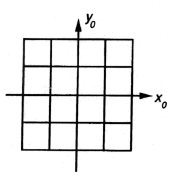
\includegraphics{figures/dist-1.png}
	\caption{Ideális eset}
  \end{subfigure}
\begin{subfigure}[b]{.32\linewidth}
	\centering
	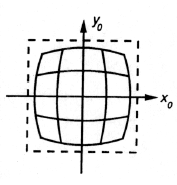
\includegraphics{figures/dist-2.png}
	\caption{,,Hordó-torzítás''}
  \end{subfigure}
\begin{subfigure}[b]{.32\linewidth}
	\centering
	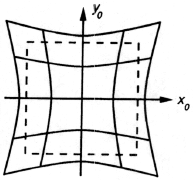
\includegraphics{figures/dist-3.png}
	\caption{,,Tűpárna-torzítás''}
  \end{subfigure}
\caption{Lencsék radiális torzítása \cite{distortion} \label{fig:radial-distortion}}
\end{figure}

A gyakorlatban gyakran használt modell, hogy a radiális torzítás esetében a torzított és a javított pontok között egy polinomfüggvény teremt kapcsolatot:

\[\left[\begin{array}{c}x_{\hbox{\small jav}}\\ y_{\hbox{\small jav}}\end{array}\right] = (1 + k_1r^2 + k_2r^4 + k_3r^6) \left[\begin{array}{c}x\\y\end{array}\right]\]

ahol $(x,y)$ volt az eredeti kép egy pixelének koordinátája, és $(x_{\hbox{\small jav}}, y_{\hbox{\small jav}})$ pedig az új koordináta a korrigált képen. Tangenciális torzítás pedig a következő egyenletek segítségével javítható:
\[x_{\hbox{\small jav}} = x + \Big(2p_1xy + p_2(r^2+2x^2)\Big)\]
\[y_{\hbox{\small jav}} = y + \Big(p_1(r^2+2y^2) + 2p_2xy\Big)\]
Ekkor $k_1, k_2$ és $k_3$ a radiális, $p_1$ és $p_2$ pedig a tangenciális torzítás együtthatói.

Kalibrálás során ezeket az együtthatókat határozzuk meg. A képen szereplő egyenesek görbületét, mint költség-függvényt minimalizálva, kiszámolhatjuk a radiális torzítást, hiszen ideális esetben nincs görbület. A gyakorlatban ez úgy történik, hogy egy előre ismert objektumot -- például egy sakktáblát -- detektálunk a képeken (lásd \aref{fig:chessboards}. ábra), és a sarokpontokat összekötő egyeneseket vizsgáljuk.

\begin{figure}[tbh]
\centering
\begin{subfigure}[b]{0.49\linewidth}
	\centering
	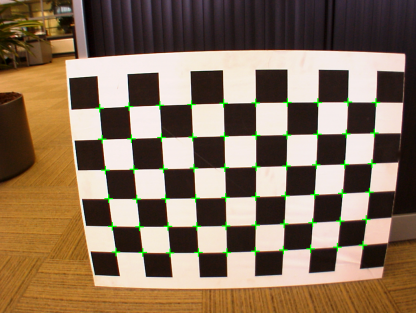
\includegraphics[width=200pt]{figures/distorted.png}
	\caption{Kamera képe, sarokpontokkal}
  \end{subfigure}
\begin{subfigure}[b]{0.49\linewidth}
	\centering
	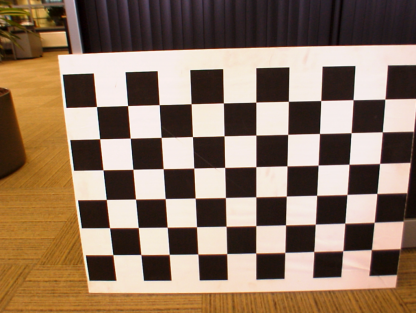
\includegraphics[width=200pt]{figures/undistorted.png}
	\caption{Javított kép}
  \end{subfigure}
\caption{Radiális torzítás meghatározása \cite{pinhole-model} \label{fig:chessboards}}
\end{figure}

Az előzőekben a kamera \textit{belső paramétereit} vizsgáltuk, melyeket a kamera lencséi és fókusztávolsága határoznak meg. Azonban szükséges beszélnük a \textit{külső paraméterekről} is, amely a kamera pozícióját és irányát mutatja a világ-koordinátához képest.

A gyakorlatban a kamera helyét és irányát egy $\mathbf{c}(c_1, c_2, c_3)$ vektorral és egy $\mathbf{R}$ forgatási mátrixszal adjuk meg. Így ahhoz, hogy egy 3D-s pont képét megkapjuk, először a kamerát el kell tolni a világkoordináta-rendszer origójába, majd forgatni, vagyis:

\[s \left[\begin{array}{c}
u \\ 
v \\
1
\end{array}\right] = \left[\begin{array}{cccc}
f & 0 & o_x & 0 \\ 
0 & f & o_y & 0 \\
0 & 0 & 1 & 0
\end{array}\right] \left[\begin{array}{cccc}
r_{11} & r_{12} & r_{13} & 0 \\ 
r_{21} & r_{22} & r_{23} & 0 \\ 
r_{31} & r_{32} & r_{33} & 0 \\ 
0 & 0 & 0 & 1 \\ 
\end{array}\right] \left[\begin{array}{cccc}
1 & 0 & 0 & -c_1 \\ 
0 & 1 & 0 & -c_2 \\ 
0 & 0 & 1 & -c_3 \\ 
0 & 0 & 0 & 1 \\ 
\end{array}\right] \left[\begin{array}{c}
X \\ 
Y \\
Z \\
1
\end{array}\right]\]

A két transzformácó összevonása után:

\[s \left[\begin{array}{c}
u \\ 
v \\
1
\end{array}\right] = \left[\begin{array}{cccc}
f & 0 & o_x & 0 \\ 
0 & f & o_y & 0 \\
0 & 0 & 1 & 0
\end{array}\right] \left[\begin{array}{cc}
\mathbf{R} & -\mathbf{R} \mathbf{c}^T \\ 
\mathbf{0} & 1 \\ 
\end{array}\right] \left[\begin{array}{c}
X \\ 
Y \\
Z \\
1
\end{array}\right]\]

$\mathbf{t}^T = -\mathbf{R}\mathbf{c}^T$ helyettesítéssel, valamint a fókusztávolságot az effektív pixelméretekkel beszorozva kapjuk \cite{camera-calib}-ben is található egyenletet:

\[s \left[\begin{array}{c}
u \\ 
v \\
1
\end{array}\right] = \underbrace{\left[\begin{array}{ccc}
f_x & 0 & o_x \\ 
0 & f_y & o_y \\
0 & 0 & 1
\end{array}\right]}_{\mathbf{A}} \left[\begin{array}{ccc|cc}
r_{11} & r_{12} & r_{13} & t_1 \\ 
r_{21} & r_{22} & r_{23} & t_2 \\
\undermat{\mathbf{R}}{r_{31} & r_{32} & r_{33}} & t_3 \\
\end{array}\right] \left[\begin{array}{c}
X \\ 
Y \\
Z \\
1
\end{array}\right]\]
ahol:
\begin{itemize}[itemsep=0pt]
\item $s$ a homogén skálázási tényező
\item $\mathbf{A}$ a kamera-mátrix (\textit{belső paraméterek mátrixa})
\item $(o_x, o_y)$ a főpont képsíkbeli koordinátája, amely általában a kép közepe
\item $(f_x, f_y)$ pedig a fókusztávolságok pixelekben kifejezve
\item $\mathbf{R}$ a forgatási mátrix és $\mathbf{t} = (t_1, t_2, t_3)$ az eltolás-vektor -- együttesen $\Big[\,\mathbf{R}\,|\,\mathbf{t}^T\,\Big]$ a forgatás-eltolás mátrix, mely a \textit{külső paraméterek mátrixa}; azt határozza meg, hogy a statikus világhoz képest a kamera hol helyezkedik el, vagy fordítva, a statikus kamerához a világ hogyan van pozícionálva.
\end{itemize}

A kamera külső paramétereit, a belső paraméterekhez hasonlóan kalibrálással kapjuk meg. A kalibráláshoz egy ismert objektumot használunk fel, ugyanúgy ahogy előbb, most is használhatunk egy sakktáblát. A sakktábla sarokpontjait a világ-koordinátarend\-szerben koordinátázva (pl. minden pontnak a 3. koordinátája fixen 0), valamint ezek képeit a kamera képein több állásban detektálva meghatározható $\mathbf{R}$ és $\mathbf{t}$ \cite{camera-calib}.

    %----------------------------------------------------------------------------
\chapter{Több kamerából álló kamera-rendszerek}
%----------------------------------------------------------------------------

A kitűzött feladat szempontjából két fontos részproblémát kell több kamerából álló rendszerek esetén megoldani. Az első a kamerák szinkronizációjának problémája, ami akkor merül fel, ha a kamerák nem egy közös feldolgozó egységhez kapcsolódnak, hanem például a kamerák képeit egy videófolyamként kapjuk. A második pedig, hogy a kamerák képei alapján a háromdimenziós teret, vagy annak egy részét a lehető legjobban rekonstruáljuk. Ez a fejezet ezen két problémát járja körbe, valamint végül bemutat egy megoldást a mozgó objektumok detekciójára.

\section{Kamerák szinkronizációja}

Amennyiben a videófolyamba időpecséteket kódolunk, a kamerák szinkronizációja megoldható. A képsorokat a kódolt információ alapján egymáshoz tudjuk időzíteni, feltéve, hogy a kamerák óráit már előtte szinkronizáltuk.

Amennyiben ilyen adat nem áll rendelkezésre a videófolyamban, egyéb módszert kell keresnünk. Megoldás lehet, ha a kamerák képsorain egy közös trigger-eseményt keresünk. Az Önálló laboratórium 1. című tárgy keretében \cite{onlab-1} egy lézerpontot kerestem mindegyik képen, és a felvillanás időpontját tekintettem referenciának. Ehhez nagyon hasonló a filmiparban használt \textit{clapperboard}, aminek összeütését használják szinkronizációra, de akár egy egyszerű taps is megfelelhet, amennyiben a kamerák hangot is rögzítenek.

\section{A háromdimenziós tér rekonstrukciója \label{sec:methods}}

A dolgozat során kettő, lényegében eltérő módszerre térek ki. Az első a sztereó-látás elvén alapszik, azaz a kamerákat párosával használva -- azokat sztereó-kalibrálva -- alkotunk mélységképet, mely segítségével a képpontokat mélységinformációval ruházzuk fel. A második eljárás az optikai-folyamok segítségével a kamerák képein meghatározza az egymásnak megfelelő pontokat, és ezekből a párosításokból háromszögelés után meghatározza a pontok világbeli koordinátáját.

\subsection{Sztereó-látás, sztereó-kalibráció}

Sztereó-kalibráció \cite{camera-calib-3d} során egy már ismert háromdimenziós objektumot használunk fel, és attól függően, hogy az objektum ismert pontjait a két kamera képén hol látjuk, kiszámolhatjuk a kamerák belső és külső paramétereit (lásd előző fejezet), valamint a kamerák egymáshoz való viszonyát (eltolás, forgatás). 

Tekintsünk két kamerát, ami ugyanazt a térrészt veszi más szögből, lásd \aref{fig:epipolar}. ábrát.

\begin{figure}[tbh]
\centering
\tdplotsetmaincoords{30}{130}
\begin{tikzpicture}[line join = round, line cap = round, >=triangle 45, tdplot_main_coords]
  
  \coordinate (O) at (0, 0, 0);
  
  % kocka
  
  \coordinate (C2) at (-3.5, -1, 1);
  \node [cross] at (C2) {};
  \node [above] at (C2) {\small $P$};
  
  % képsík
  
  \coordinate (I1) at (0, 0, 0);
  \coordinate (I2) at (0, 4, 0);
  \coordinate (I3) at (0, 4, 3);
  \coordinate (I4) at (0, 0, 3);

  \coordinate (_I1) at (-0.7, 5, 0);
  \coordinate (_I2) at (-0.7, 5, 3);
  \coordinate (_I3) at (-4.7, 5, 3);
  \coordinate (_I4) at (-4.7, 5, 0);


  \draw (I1) -- (I2);
  \draw (I2) -- (I3);
  \draw (I3) -- (I4);
  \draw (I4) -- (I1);
  
  \draw (_I1) -- (_I2);
  \draw (_I2) -- (_I3);
  \draw (_I3) -- (_I4);
  \draw (_I4) -- (_I1);

  \coordinate (UV) at (0, 1.1, 1.35);
  \node [cross] at (UV) {};
  \node [left] at (UV) {\small $p_1$};

  \coordinate (UV2) at (-2.86, 5, 1.4);
  \node [cross] at (UV2) {};
  \node [right] at (UV2) {\small $p_2$};

  % optikai tengely
  \coordinate (E1) at (0, 3.6071, 1.5);
  \coordinate (C1) at (1.5, 2, 1.5);
  \coordinate (A1) at (-1, 2, 1.5);

  \coordinate (E2) at (-1.3, 5, 1.5);
  \coordinate (C2_) at (-2.7, 6.5, 1.5);
  \coordinate (A2) at (-2.7, 4, 1.5);

  \node [below] at (C1) {\small $C_1$};
  \node [below] at (C2_) {\small $C_2$};
  \node [cross] at (E1) {};
  \node [cross] at (E2) {};
  \node [below] at (E1) {\small $e_1$};
  \node [below] at (E2) {\small $e_2$};
  
  \draw [dashed,shorten >=-20pt,shorten <=-20pt] (UV) -- (E1);
  \draw [dashed,shorten >=-20pt,shorten <=-20pt] (UV2) -- (E2);

  % leképezés
  
  \draw [dotted] (C1) -- (C2);
  \draw [dotted] (C2_) -- (C2);
  \draw [dotted] (C1) -- (C2_);
  
  \node at (-2, 2.5, 1) {$\pi$};
  
\end{tikzpicture}
\caption{Epipoláris geometria szemléltetése \label{fig:epipolar}}
\end{figure}

A $P$ pont az első kamera $I_1$ képén $p_1$-be, a második kamera $I_2$ képén $p_2$-be képződik le. Visszafele gondolkozva, ha megvan egy pontnak két képe a két képsíkon, akkor a kamera középpontjait összekötve ezekkel a képpontokkal két félegyenest (sugarat, az angol \textit{ray} szóból) kapunk, melyek metszéspontjában kereshető a valódi $P$ pont (háromszögelés). Fontos megjegyezni, hogy ilyen metszéspont csak ideális esetben létezik, a gyakorlatban nagyon ritkán. Ilyenkor a kitérő félegyenesek közti legrövidebb szakasz középpontját tekintjük a ,,metszéspontnak''.

Nyilvánvaló, hogy $C_1$, $C_2$, $P$, valamint $p_1$ és $p_2$ egy síkon van rajta, ezt \textit{epipoláris sík}nak nevezzük, az ábrán $\pi$-vel jelölve (lásd pontozott vonal által határolt háromszög). Ezt felhasználva adódik, hogy egy $p_1$ pont párja a másik, $I_2$ képsíkon nem lehet máshol, mint $I_2$ és $\pi$ metszésvonalán. Ezeket, vagyis a képsíkok és az epipoláris síkok metszéspontját \textit{epipoláris egyeneseknek} nevezzük, melyeket szaggatott vonalak jelölnek az ábrán.

Ebből következik, hogy a képpontok párját a másik képen elég csak az epipoláris egyeneseken keresni, mert az előzőek alapján csak ott lehetnek. További egyszerűsítés, ha ezek az epipoláris egyenesek mindannyian párhuzamosak és vízszintesek, hiszen ekkor a képeken csak $x$ irányban kell keresni a pontok megfelelőit a másik képen. Gyakorlatban, nagyon nehéz így beállítani a kamerákat, ezért a kamerák képeit úgy transzformálják, hogy egy képzeletbeli közös síkba essenek a képsíkok, ahol már teljesül ez a feltétel. Ezt \textit{rektifikációnak} hívják, lásd \aref{fig:rectification}. ábrát.

\begin{figure}[tbh]
\centering
\begin{subfigure}[b]{.49\textwidth}
\centering
\tdplotsetmaincoords{30}{130}
\begin{tikzpicture}[line join = round, line cap = round, >=triangle 45, tdplot_main_coords]
  
  % képsík
  
  \coordinate (I1) at (0, 0, 0);
  \coordinate (I2) at (0, 3, 0);
  \coordinate (I3) at (0, 3, 3);
  \coordinate (I4) at (0, 0, 3);

  \coordinate (_I1) at (-0.7, 4, 0);
  \coordinate (_I2) at (-0.7, 4, 3);
  \coordinate (_I3) at (-3.7, 4, 3);
  \coordinate (_I4) at (-3.7, 4, 0);


  \draw (I1) -- (I2);
  \draw (I2) -- (I3);
  \draw (I3) -- (I4);
  \draw (I4) -- (I1);
  
  \draw (_I1) -- (_I2);
  \draw (_I2) -- (_I3);
  \draw (_I3) -- (_I4);
  \draw (_I4) -- (_I1);

  \coordinate (C1) at (1.5, 1.5, 1.5);
  \coordinate (C2_) at (-2.2, 5.5, 1.5);

  \node [below] at (C1) {\small $C_1$};
  \node [below] at (C2_) {\small $C_2$};

  % leképezés

  \draw [dashed,shorten >=-10pt] (C1) -- (I1);
  \draw [dashed,shorten >=-10pt] (C1) -- (I2);
  \draw [dashed,shorten >=-10pt] (C1) -- (I3);
  \draw [dashed,shorten >=-10pt] (C1) -- (I4);
  \draw [dashed,shorten >=-10pt] (C2_) -- (_I1);
  \draw [dashed,shorten >=-10pt] (C2_) -- (_I2);
  \draw [dashed,shorten >=-10pt] (C2_) -- (_I3);
  \draw [dashed,shorten >=-10pt] (C2_) -- (_I4);
  
\end{tikzpicture}
\caption{Rektifikáció előtt a képsíkok}
\end{subfigure}\begin{subfigure}[b]{.49\textwidth}
\centering
\tdplotsetmaincoords{20}{90}
\begin{tikzpicture}[line join = round, line cap = round, >=triangle 45, tdplot_main_coords]
  
  % képsík
  
  \coordinate (I1) at (0, 0, 0);
  \coordinate (I2) at (0, 2, 0);
  \coordinate (I3) at (0, 2, 3);
  \coordinate (I4) at (0, 0, 3);

  \coordinate (_I1) at (0, 3, 0);
  \coordinate (_I2) at (0, 5, 0);
  \coordinate (_I3) at (0, 5, 3);
  \coordinate (_I4) at (0, 3, 3);
  
  \coordinate (S1) at (0, -0.5, -1);
  \coordinate (S2) at (0, 5.5, -1);
  \coordinate (S3) at (0, 5.5, 4);
  \coordinate (S4) at (0, -0.5, 4);

  \draw (I1) -- (I2);
  \draw (I2) -- (I3);
  \draw (I3) -- (I4);
  \draw (I4) -- (I1);
  
  \draw (_I1) -- (_I2);
  \draw (_I2) -- (_I3);
  \draw (_I3) -- (_I4);
  \draw (_I4) -- (_I1);

  \draw [dotted] (S1) -- (S2);
  \draw [dotted] (S2) -- (S3);
  \draw [dotted] (S3) -- (S4);
  \draw [dotted] (S4) -- (S1);
  
  \coordinate (C1) at (1.5, 1, 1.5);
  \coordinate (C2_) at (1.5, 4, 1.5);

  % leképezés

  \draw [dashed,shorten >=-10pt] (C1) -- (I1);
  \draw [dashed,shorten >=-10pt] (C1) -- (I2);
  \draw [dashed,shorten >=-10pt] (C1) -- (I3);
  \draw [dashed,shorten >=-10pt] (C1) -- (I4);
  \draw [dashed,shorten >=-10pt] (C2_) -- (_I1);
  \draw [dashed,shorten >=-10pt] (C2_) -- (_I2);
  \draw [dashed,shorten >=-10pt] (C2_) -- (_I3);
  \draw [dashed,shorten >=-10pt] (C2_) -- (_I4);
  
\end{tikzpicture}
\caption{Egy síkba transzformálva}
\end{subfigure}
\caption{Rektifikáció szemléltetése \label{fig:rectification}}
\end{figure}

\Aref{fig:stereo-calibration-before}. és \aref{fig:stereo-calibration-after}. ábrán látható, ahogy egy sakktábla-mintát (melynek valódi koordinátái ismertek), több szögből lefotózva a rektifikáció \cite{camera-calib-3d} előtt és után, hogy alakul a két kamera képe. A piros segéd egyenesek segítségével az is jó látható, hogy a rektifikáció után az egymásnak megfelelő rácspontok valóban egy vízszintes egyenesre esnek.

\begin{figure}[tbh]
  \centering
  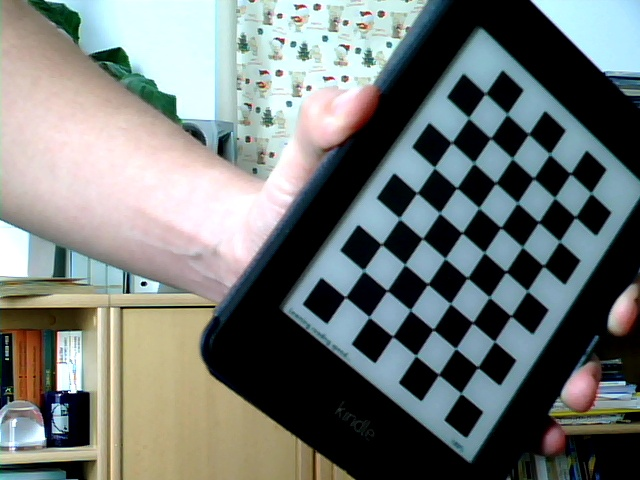
\includegraphics[width=160pt]{figures/left07.jpg}\hspace{10pt}
  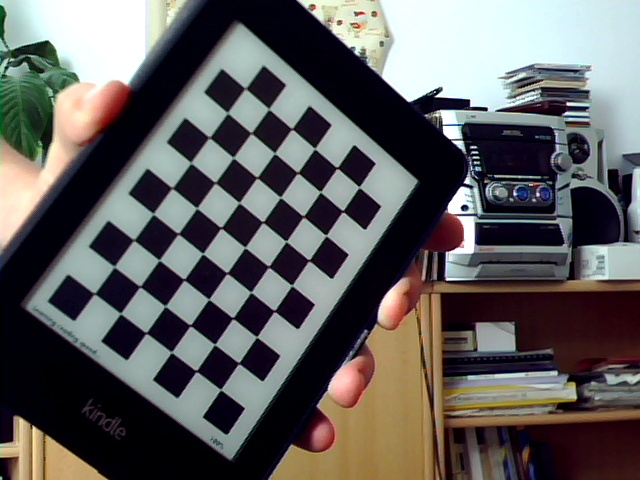
\includegraphics[width=160pt]{figures/right07.jpg}
  \caption{A kalibrációhoz felhasznált egyik képpár   \label{fig:stereo-calibration-before}}
\end{figure}

\begin{figure}[tbh]
  \centering
\begin{tikzpicture}[x=330,y=330]
	\node[anchor=south west,inner sep=0] at (0.515151,0) {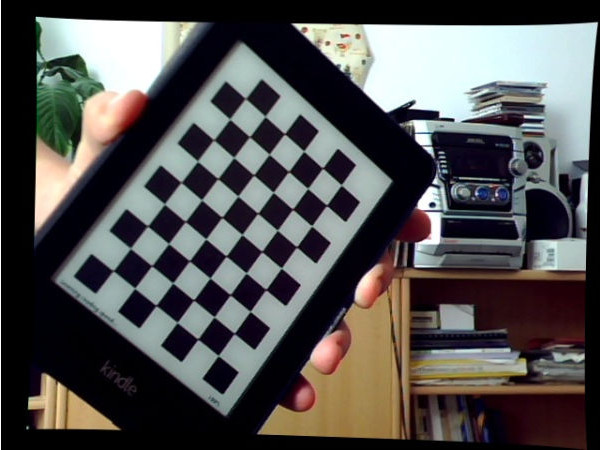
\includegraphics[width=160pt] {figures/calibrated_right.jpg}};
    \node[anchor=south west,inner sep=0] at (0,0) {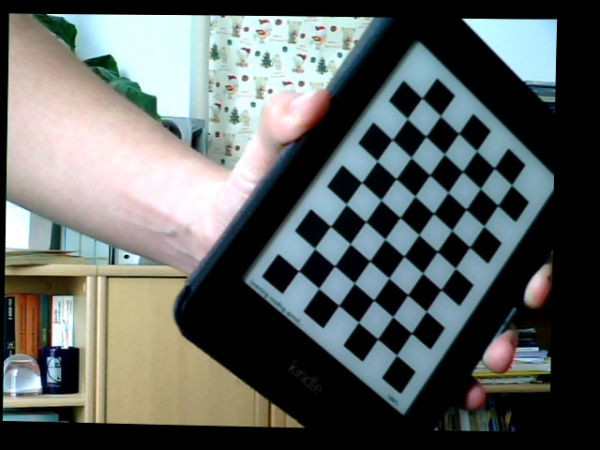
\includegraphics[width=160pt]    {figures/calibrated_left.jpg}};
    \draw[red,thick] (0,0.301) -- (1,0.301);
    \draw[red,thick] (0,0.200) -- (1,0.200);
    \draw[red,thick] (0,0.140) -- (1,0.140);
    \draw[red,thick] (0,0.045) -- (1,0.045);
\end{tikzpicture}
  \caption{Rektifikáció után a két kamera képe \label{fig:stereo-calibration-after}}
\end{figure}

A rektifikált képpárokra pedig már léteznek algoritmusok \cite{SGBM, stereo-var}, melyek megtalálják a képeken az egymásnak megfelelő pontokat és az elmozdulásuk alapján megadják a pontok mélységértékeit. \Aref{fig:depth-showcase}. ábra segítségével könnyű látni, hogy a nagy elmozdulást mutató pontok közelebb, a kisebbek távolabb találhatóak a kamerától.

\begin{figure}[tbh]
  \centering
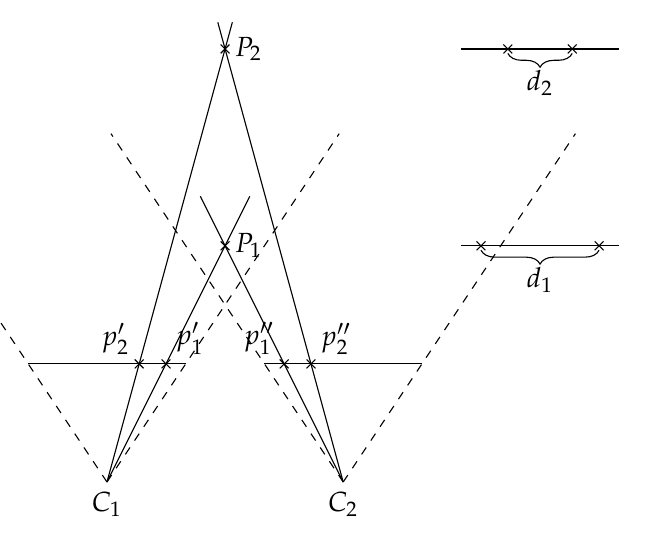
\begin{tikzpicture}

\tikzset{
    position label/.style={
       below = 3pt,
       text height = 1.5ex,
       text depth = 1ex
    },
   brace/.style={
     decoration={brace,amplitude=5pt},
     decorate
   }
}

  \coordinate (L1) at (0, 0);
  \coordinate (L2) at (2, 0);
  \draw (L1) -- (L2);
  
  \coordinate (C1) at (1, -1.5);
  \node [below] at (C1) {$C_1$};

  \draw [dashed, shorten >= -100pt] (C1) -- (L1);
  \draw [dashed, shorten >= -100pt] (C1) -- (L2);

  
  \coordinate (R1) at (3, 0);
  \coordinate (R2) at (5, 0);
  \draw (R1) -- (R2);
  
  \coordinate (C2) at (4, -1.5);
  \node [below] at (C2) {$C_2$};

  \draw [dashed, shorten >= -100pt] (C2) -- (R1);
  \draw [dashed, shorten >= -100pt] (C2) -- (R2);

  \coordinate (P1) at (2.5, 1.5);
  \node [cross] at (P1) {};
  \node [right] at (P1) {$P_1$};
  
  \coordinate (P2) at (2.5, 4);
  \node [cross] at (P2) {};
  \node [right] at (P2) {$P_2$};

  \draw [shorten >= -20pt] (C1) -- (P1);
  \draw [shorten >= -10pt] (C1) -- (P2);
  \draw [shorten >= -20pt] (C2) -- (P1);
  \draw [shorten >= -10pt] (C2) -- (P2);
  
  \coordinate (P2B) at (1.4090, 0);
  \node [cross] at (P2B) {};
  \node [above left] at (P2B) {$p_2'$};
  
  \coordinate (P1B) at (1.75, 0);
  \node [cross] at (P1B) {};
  \node [above right] at (P1B) {$p_1'$};
  
  \coordinate (P2J) at (3.591, 0);
  \node [cross] at (P2J) {};
  \node [above right] at (P2J) {$p_2''$};
  
  \coordinate (P1J) at (3.25, 0);
  \node [cross] at (P1J) {};
  \node [above left] at (P1J) {$p_1''$};
  
  % távolságok másolata
  
  \draw (5.5, 4) -- (7.5, 4);
  \node [cross] (T1) at (6.9090, 4) {};
  \node [cross] (T2) at (6.091, 4) {};
  \draw (5.5, 1.5) -- (7.5, 1.5);
  \node [cross] (B1) at (7.25, 1.5) {};
  \node [cross] (B2) at (5.75, 1.5) {};
  
   \draw [brace] (T1.south) -- (T2.south) node [position label, pos=0.5] {$d_2$};
   \draw [brace] (B1.south) -- (B2.south) node [position label, pos=0.5] {$d_1$};
  
\end{tikzpicture}
  \caption{Elmozdulás és mélység kapcsolata; a kameráktól távolabbi $P_2$ pont képeinek $d_2$ távolsága kisebb, mint a közelebbi $P_1$ pont képeinek $d_1$ távolsága \label{fig:depth-showcase}}
\end{figure}

Fontos megemlíteni, hogy gyakorlatban a kameráknak már eleve nagyon közel kell lenniük az ideális elhelyezkedéshez, azaz, egymás mellett (vagy egymás felett, attól függően, hogy horizontális, vagy vertikális sztereó-kamerákat használunk) legyenek, úgy hogy képsíkjuk közel egybeessenek. Így érhető el az, hogy a rektifikáció sikeres legyen, valamint, hogy utána a kép legnagyobb része ,,használható'' legyen, lásd \aref{fig:stereo-calibration-after}. ábrán a szélén lévő fekete részeket.

\subsection{Optikai-folyam \label{methods:optic}}

Az előzőekben megismert eljárás azt feltételezi, hogy a kamerák párosával sztereó-kalib\-ráltak, és ezt kihasználva számol mélységképet a kalibráció során felhasznált segéd-objek\-tum alapján.

A most ismertetésre kerülő eljárás, az \textit{optikai-folyam}okat \cite{optic-flow} hívja segítségül. Vegyünk egymás utáni képsorokat egy mozgó objektumról. Az objektum mindegyik pontja egy háromdimenziós $\mathbf{P}(t)$ útvonalon mozog, mely a kamerák képén egy $\mathbf{p}(t) = \big(x(t), y(t)\big)$ kétdimenziós útvonalnak feleltethető meg. Minden pontra nézve az elmozdulás $d\mathbf{p}(t) / dt$ irányát egy vektormezőt kapunk, ezt hívjuk optikai-folyamnak.

Jelöljük $I(x, y, t)$-vel a kép $(x, y)$ pontjának intenzitását a $t$ időpillanatban. Feltehető, hogy két egymás utáni képkockán ugyanazon pont képpontjainak intenzitása konstans (\textit{világosság állandóság}, az angol \textit{brightness constancy} kifejezésből), vagyis:
\[I(x, y, t) = I(x+dx, y+dy, t+dt)\]
ahol az $(x,y)$ képpont $dt$ idő alatt $(dx,dy)$-nal mozdult el. A jobb oldal jól közelíthető az első-rendű Taylor-sor kifejtésével:

\[I(x+dx, y+dy, t+dt) \approx I(x, y, t) + \frac{\partial I}{\partial x} dx + \frac{\partial I}{\partial y} dy + \frac{\partial I}{\partial t} dt\]

Felhasználva a világosság állandóság kényszert:

\[\frac{\partial I}{\partial x} dx + \frac{\partial I}{\partial y} dy + \frac{\partial I}{\partial t} dt = 0\]

Mindkét oldalt $dt$-vel osztva:

\[\frac{\partial I}{\partial x} \frac{dx}{dt} + \frac{\partial I}{\partial y} \frac{dy}{dt} + \frac{\partial I}{\partial t} \frac{dt}{dt} = 0\]

Végül bevezetve a $\nabla \mathbf{I} = \left(\frac{\partial I}{\partial x}, \frac{\partial I}{\partial y}\right)$ és $\mathbf{V} = \left(\frac{dx}{dt}, \frac{dy}{dt}\right)$ jelöléseket, az alábbi egyszerű alakot ölti:

\[\nabla \mathbf{I} \cdot \mathbf{V} = -\frac{\partial I}{\partial t}\]

Ezt nevezzük az optikai folyam feltételi egyenletének \cite{phd}. Mivel $\mathbf{V}\left(\frac{dx}{dt}, \frac{dy}{dt}\right)$ nem ismert, ezért egy egyenletben két ismeretlenünk van, így az optikai-folyam általános esetben nem oldható meg.

\subsubsection{Lucas-Kanade módszer \cite{LK}}

Ez a módszer ritka vektor-mezőt generál a jellegzetes pontok elmozdulására. Lényege, hogy a vizsgált pontok és azok környezetében az elmozdulás azonos \cite{lk-wiki}, vagyis:

\[\nabla \mathbf{I}_{\mathbf{q_1}} \cdot \mathbf{V} = -\frac{\partial I}{\partial t}(\mathbf{q_1}, t)\]
\[\nabla \mathbf{I}_{\mathbf{q_2}} \cdot \mathbf{V} = -\frac{\partial I}{\partial t}(\mathbf{q_2}, t)\]
\[\vdots\]
\[\nabla \mathbf{I}_{\mathbf{q_n}} \cdot \mathbf{V} = -\frac{\partial I}{\partial t}(\mathbf{q_n}, t)\]

ahol $\mathbf{q_1},\mathbf{q_2},\ldots,\mathbf{q_n}$ a vizsgált pont környezetében lévő pontok és $\nabla \mathbf{I}_{\mathbf{q_i}} = \left(\frac{\partial I}{\partial x}(\mathbf{q_i}), \frac{\partial I}{\partial y}(\mathbf{q_i})\right)$. Ez így viszont már egy túlhatározott egyenletrendszer, melyhez közelítő megoldás a legkisebb-négyzetek módszerével kereshető \cite{LK, lk-wiki}. A gyakorlatban a követendő pontokra a Shi-Thomasi \cite{shi-thomasi} módszer által adott sarokpontokat szokták használni (lásd \aref{fig:lk}. ábra).

%Ez önmagában így csak kis mozgásokat tud követni, ezért nagy mozgások esetén a piramis-módszert használjuk; amikor is a képeket több lépcsőben kicsinyítjük, és ezeken is lefuttatjuk az algoritmusokat (ekkor a kis mozgások eltűnnek, a nagyok pedig kisebbekké válnak).

\begin{figure}[tbh]
\centering
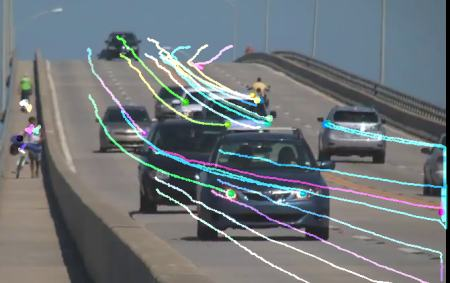
\includegraphics[width=300pt]{figures/opticalflow_lk.jpg}
\caption{Minta a sarokpontok követésére \cite{opencv-lk} \label{fig:lk}}
\end{figure}

\subsubsection{Gunner Farnebäck módszer \cite{farneback}}

A módszer lényege, hogy a kép pixeleinek intenzitását egy polinommal közelíti:

\[f(\mathbf{x}) \sim \mathbf{x}^T \mathbf{A} \mathbf{x} + \mathbf{b}^T \mathbf{x} + c\]

ahol $\mathbf{A}$ egy szimmetrikus mátrix, $\mathbf{b}$ vektor és $c$ skalár.

Ezeket az együtthatókat a legkisebb-négyzetek módszerével közelítően meghatározhatjuk. Feltéve, hogy a teljes kép egyetlen polinommal felírható, és a két képkockán az egész polinom ideálisan $\mathbf{d}$-vel mozdul el:

\[f_1(\mathbf{x} - \mathbf{d}) = f_2(\mathbf{x})\]

A fenti képlet jelenti a világosság állandóság kényszer teljesülését. Bal oldalt kifejtve, jobb oldalt pedig átírva a polinom-alakba \cite{farneback}:

\[\mathbf{x}^T \mathbf{A}_1 \mathbf{x} + (\mathbf{b_1} - 2 \mathbf{A}_1\mathbf{d})^T \mathbf{x} + \mathbf{d}^T \mathbf{A}_1 \mathbf{d} -\mathbf{b}_1^T + c_1 = \mathbf{x}^T \mathbf{A}_2 \mathbf{x} + \mathbf{b_2}^T \mathbf{x} + c_2\]

Az együtthatókat egyenlővé téve, kapjuk a következő egyenleteket:

\[\begin{array}{rcl}\mathbf{A}_2 &=& \mathbf{A}_1\\\mathbf{b_2} &=& \mathbf{b_1} - 2 \mathbf{A}_1\mathbf{d}\\ c_2 &=& \mathbf{d}^T \mathbf{A}_1 \mathbf{d} -\mathbf{b}_1^T + c_1 \end{array}\]

Jól látható, hogy $\mathbf{d}$ meghatározható ha $\mathbf{A}_1$ determinánsa nem nulla. Általános esetben természetesen nem élhetünk az előbbi feltételekkel, miszerint mindkét kép leírható egyetlen polinommal és ideálisan minden pont $\mathbf{d}$-vel mozdult el. Ezért lokális polinomokkal dolgozunk, melyek a pontok egy környezetében érvényesek, vagyis $\mathbf{A}_1(\mathbf{x}), \mathbf{b_1}(\mathbf{x}),$ $c_1(\mathbf{x})$ és $\mathbf{A}_2(\mathbf{x}), \mathbf{b_2}(\mathbf{x}), c_2(\mathbf{x})$ együtthatókkal kell számolunk. Ekkor az alábbi közelítéseket téve:
\[\mathbf{A}(\mathbf{x}) = \frac{\mathbf{A}_2(\mathbf{x}) + \mathbf{A}_2(\mathbf{x})}{2}\]
\[\Delta \mathbf{b}(\mathbf{x}) = -\frac{1}{2}\left(\mathbf{b}_2(\mathbf{x})-\mathbf{b}_1(\mathbf{x})\right)\]
Kapjuk az előbbi egyenletekkel összevetve a következőt:
\[\mathbf{A}(\mathbf{x})\mathbf{d}(\mathbf{x}) = \Delta \mathbf{b}(\mathbf{x})\]

Ekkor $\mathbf{d}(\mathbf{x})$ szerepében megkaptuk a vektor-mezőt. Ez az egyenlet pontonként felírva megoldható, de a gyakorlatban zajos eredményt szolgáltat. Ezt elkerülendő azzal a feltevéssel élünk, hogy a pontok egy környezetében az elmozdulás vektorok csak kicsit változnak, és így a fenti megoldása egy költség-minimalizálási problémává változik \cite{farneback}.

Ez utóbbi algoritmust \cite{opencv-lk} fogom a dolgozat során alkalmazni, mert sűrű optikai-folyamokat szolgáltat, és nem kell sarokpontokat keresni a kiinduló képen. \Aref{fig:dense-of}. ábrán látható egy példa, ami egy kanyon felett elrepülő helikopter videójának két egymás utáni képkockájából meghatározott sűrű optikai-folyamot mutatja.

\begin{figure}[tbh]
\centering
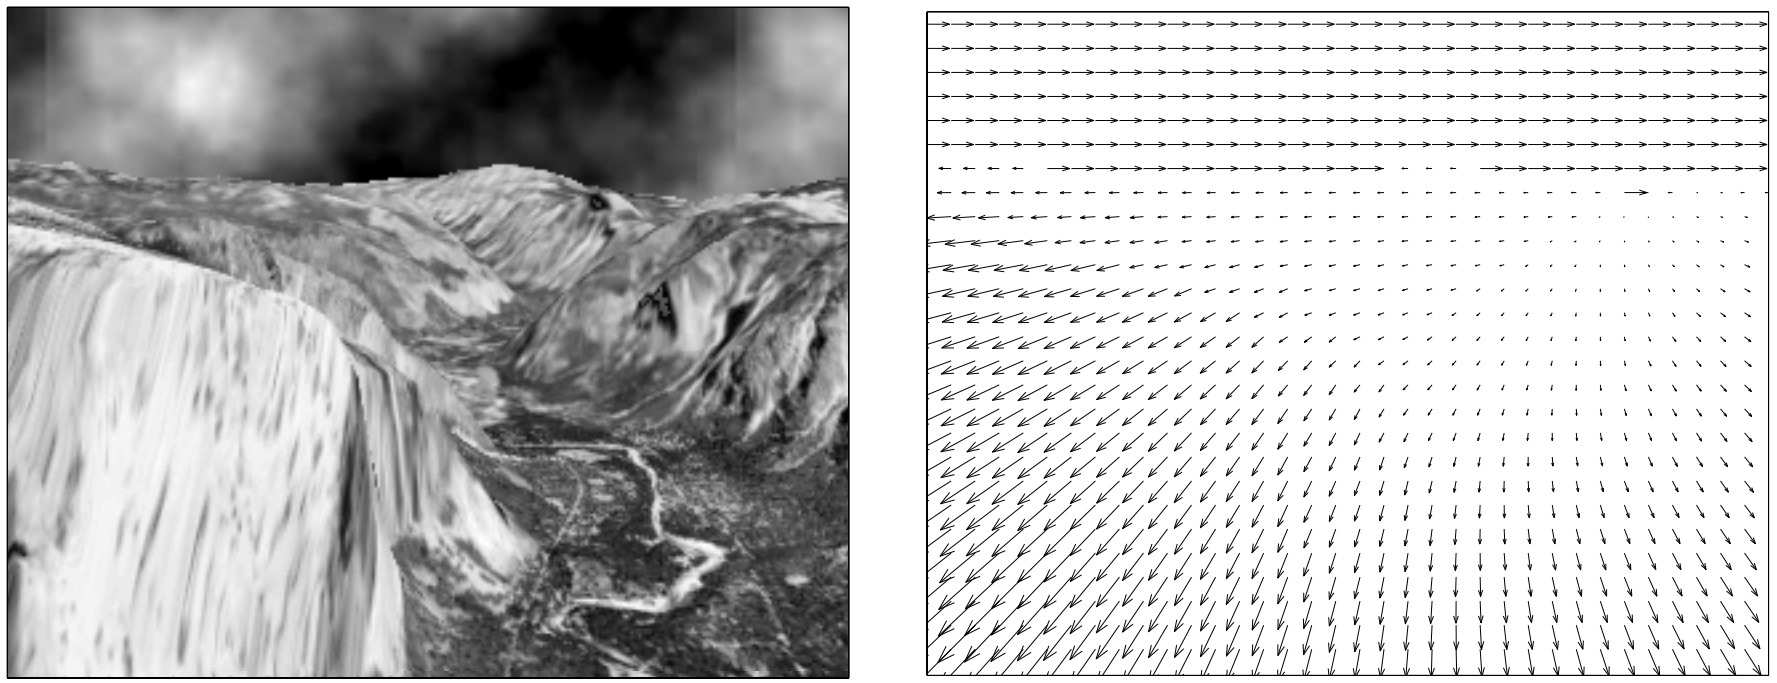
\includegraphics[width=420pt]{figures/farneback.png}
\caption{Minta sűrű optikai-folyam meghatározásra \cite{farneback} \label{fig:dense-of}}
\end{figure}

Az optikai-folyamokat felhasználhatjuk statikus objektumok (pl. szobrok, kastélyok) modellezésére, ezt a problémát \textit{structure-from-motion}-nek hívjuk \cite{sfm}. Tekintsünk egy adott objektum felé néző, de körülötte mozgó kamera két helyzetében ($C_1$ és $C_2$) látott képet (lásd \aref{fig:triangulation}. ábrát). Az objektumról a kamera mozgása során több képet készítve, és ezeken az egymásnak megfelelő pontokat az optikai-folyamok segítségével meghatározva a már említett háromszögelés módszerével meghatározhatóak a pontok háromdimenziós koordinátái, valamint a nézőpontok közötti transzformációk is \cite[4. fejezet]{book}.

\begin{figure}[tbh]
\centering
\tdplotsetmaincoords{60}{130}
\begin{tikzpicture}[line join = round, line cap = round, >=triangle 45, tdplot_main_coords]
  
  \coordinate (O) at (0, 0, 0);
  
  % kocka
  
  \coordinate (C1) at (-4.5, -2, 1);
  \coordinate (C2) at (-4.5, -1, 1);
  \coordinate (C3) at (-4.5, -1, 2);
  \coordinate (C4) at (-4.5, -2, 2);
  \coordinate (C1B) at (-5, -2, 1);
  \coordinate (C2B) at (-5, -1, 1);
  \coordinate (C3B) at (-5, -1, 2);
  \coordinate (C4B) at (-5, -2, 2);
    \node [below right] at (C2) {\small $(X, Y, Z)$};

  \draw [dashed] (C1) -- (C2);
  \draw [dashed] (C2) -- (C3);
  \draw [dashed] (C3) -- (C4);
  \draw [dashed] (C4) -- (C1);
  \draw [dashed] (C1) -- (C1B);
  \draw [dashed] (C2) -- (C2B);
  \draw [dashed] (C3) -- (C3B);
  \draw [dashed] (C4) -- (C4B);
  \draw [dashed] (C1B) -- (C2B);
  \draw [dashed] (C2B) -- (C3B);
  \draw [dashed] (C3B) -- (C4B);
  \draw [dashed] (C4B) -- (C1B);
  
  
  % képsík
  
  \coordinate (I1) at (0, 0, 0);
  \coordinate (I2) at (0, 4, 0);
  \coordinate (I3) at (0, 4, 3);
  \coordinate (I4) at (0, 0, 3);

  \coordinate (_I1) at (-0.7, 5, 0);
  \coordinate (_I2) at (-0.7, 5, 3);
  \coordinate (_I3) at (-4.7, 5, 3);
  \coordinate (_I4) at (-4.7, 5, 0);


  \draw (I1) -- (I2);
  \draw (I2) -- (I3);
  \draw (I3) -- (I4);
  \draw (I4) -- (I1);
  
  \draw (_I1) -- (_I2);
  \draw (_I2) -- (_I3);
  \draw (_I3) -- (_I4);
  \draw (_I4) -- (_I1);

  \coordinate (UV) at (0, 0.421, 1.2368);
  \node [cross] at (UV) {};

  \coordinate (UV2) at (-3.5182, 5, 1.2727);
  \node [cross] at (UV2) {};

  % optikai tengely
  \coordinate (P1) at (0, 2, 1.5);
  \coordinate (C1) at (5, 2, 1.5);
  \coordinate (A1) at (-1, 2, 1.5);

  \coordinate (P2) at (-2.7, 5, 1.5);
  \coordinate (C2_) at (-2.7, 10, 1.5);
  \coordinate (A2) at (-2.7, 4, 1.5);

  \node [below] at (C1) {\small $C_1$};
  \node [below] at (C2_) {\small $C_2$};
  \draw (C1) -- (P1);
  \draw (C2_) -- (P2);
  \node [cross] at (P1) {};
  \node [cross] at (P2) {};
  \node [below right] at (P1) {\small $P_1$};
  \node [below left] at (P2) {\small $P_2$};
  \draw [dashed,-latex] (P1) -- (A1);
  \draw [dashed,-latex] (P2) -- (A2);
  
  % leképezés
  
  \draw [dotted] (C1) -- (C2);
  \draw [dotted] (C2_) -- (C2);
  
  \draw [shorten <= 10pt, shorten >= 10pt,dashed,->,>=stealth'] (C1) to[out=-20,in=-160] (C2_);
  
\end{tikzpicture}
\caption{Mozgó kamera két állapotban \label{fig:triangulation}}
\end{figure}

Ennél lényegesen eltérő felhasználási mód, ha az optikai-folyamokat nem egy mozgó kamera két képkockáján, hanem két különböző kamera egy időponthoz tartozó két képkockáján határozzuk meg, melyek megközelítőleg ugyanazon térrészt veszik, de kicsit más pontból és szögből. Ekkor az optikai folyam lényegében a két kamera képén egy megfeleltetést tesz lehetővé. Feltéve, hogy előzetesen a kamerák pozícióját meghatároztuk (külső paraméterek), valamint ismerjük a projekciójukat leíró mátrixokat (belső paraméterek), akkor az egyező képontokat felhasználva háromszögeléssel kaphatjuk a mindkét kamera által látott pontok világbeli koordinátájukat.

Az előbbi módszer, jól használható nagy felbontású képeknél, ahol az objektum a kép nagy részét teszi ki, így sok hasznos képpontot gyűjthetünk. A feladatom során éppen ellenkezőleg, a képek csak egy részén megjelenő és ott mozgó objektumokat kell rekonstruálni, így az utóbbi megközelítést valósítom meg.

%----------------------------------------------------------------------------
\section{Objektum-detekció}
%----------------------------------------------------------------------------

A feladat megoldása során mozgó objektumokat kell követnem, azokat modelleznem, így szükség van ezeknek az egymás utáni képkockákon történő azonosítására.

{\color{red} Ezt lehet ki kell majd venni... }
Az előző részben leírt Farnebäck-módszert egy kamera egymás utáni képkockáin felhasználva becslést kaphatunk arra vonatkozóan, hogy hol lehetnek a mozgó tárgyak. A kamerák statikus helyzete révén, a háttér képpontjaihoz tartozóan közel zéró elmozdulást várunk, míg a mozgó részeken ettől eltérőt.

Azonban ez önmagában még nem elég, szükség van egy háttér-előtér szegmentálási algoritmus (MOG) \cite{MOG} felhasználására is, mely az egymás utáni képkockákból egy háttér-modellt épít. Az aktuális képkockából a kapott hátteret kivonva, megkapjuk az éppen aktuális előtérhez tartozó maszkot, lásd \aref{fig:mog-example}. ábrát.

\begin{figure}[tbh]
\centering
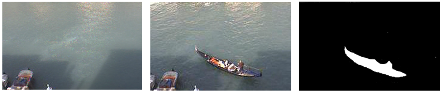
\includegraphics{figures/mog.png}
\caption{Minta a háttér-előtér elválasztási algoritmus eredményére \cite{mog-example} \label{fig:mog-example}}
\end{figure}

A választott algoritmus előnye, hogy az árnyékokat nagy valószínűséggel kiszűrí és azokat nem tekinti az objektum részének, valamint a folyamatos modellépítésnek köszönhetően, nem csak egy fix tanulási időszak alatt gyűjtött információkból határozza meg a hátteret.

A kapott előtér maszkot és az optika-folyamokat felhasználva már igen jó közelítéssel megkapjuk a mozgó objektumoknak megfelelő képszeleteket.

\section{Összefoglaló}

Ebben a fejezetben a több kamerából álló kamera-rendszerek során felmerülő és a dolgozat során is megoldandó problémákat, valamint ezek lehetséges megoldásait mutattam be. Kitértem a kamera-szinkronizációra, melyet több kamera esetén nem hagyhatunk figyelmen kívül, és leírtam két lényegében eltérő rekonstrukciós eljárást, és azok mögött meghúzódó elméleti hátteret. A fejezetet az objektum-detekció problémakörével zártam.
    %----------------------------------------------------------------------------
\chapter{Tervezés \label{chapter3}}
%----------------------------------------------------------------------------

Az elméleti megfontolások, alapelvek bemutatását követően ebben a fejezetben rátérek a feladat megoldását adó rendszer struktúrájának, főbb komponenseinek tárgyalására.

\section{A célkitűzés}

A diplomamunka során elkészített rendszernek képesnek kellett lennie egy zárt térrész tetszőlegesen választott pontjában és irányában látható, a mozgó objektumokat tartalmazó kép helyreállítására fix telepítésű kamerák valós idejű videofolyamai alapján. A helyreállítást akkor tekintettem sikeresnek, ha a mozgó objektumokat detektáltam és választott nézőpontból azok megközelítő kontúrjait sikeresen meghatároztam. A tényleges objektum struktúrájának illetve textúrájának meghatározása nem esett a dolgozat hatáskörébe. A választott nézőpontra is voltak korlátaink, érdemi rekonstrukciót csak a kamerákat összekötő képzeletbeli szakaszon és annak környezetében várhatunk, így a tesztelést is így végeztem.

A rendszer tervezése során figyelembe vettem, hogy lényegében tetszőleges számú kamerát is felhasználhattam a probléma megoldásához, ennek megfelelően a megvalósított rendszer architektúráját így készítettem el, de az elérhető eszközök korlátozott száma miatt csak két kamerával teszteltem.

Egyre több kamera bevonásával a rekonstrukció minősége, valamint a helyesen rekonstruálható nézőpontok száma növekszik, de ezzel együtt a rendszer teljesítménye a megnövekedő számítási szükséglet miatt csökken. Fontos megemlíteni, hogy a feladat és a megoldás jellegéből adódóan a független kamerákból meghatározott rekonstrukciók párhuzamosíthatóak, így ezek megfelelő feldolgozó egységet feltételezve egy időben elvégezhetőek. Ez azt jelenti, hogy a kamerák számának növelése valóban megoldás lehet a robusztusabb eredmény eléréséhez.

\section{Keretrendszer}

A diplomamunka során az OpenCV \cite{opencv} keretrendszert használtam, melynek célja, hogy a fejlesztőknek egy szabadon és ingyenes elérhető alkalmazás-könyvtárat biztosítson a gépi látás területén elterjedt és gyakran használt algoritmusokhoz. Több nyelvhez is biztosít API-t, én ezek közül a C++-os interfészét alkalmaztam, a lehető legnagyobb teljesítmény elérése érdekében. Az OpenCV-t már az előző félévekben megismertem, így a diplomamunka során már eredményesen tudtam építkezni az általa nyújtott funkciókra.

\section{A tervezett rendszer működése}

A feladat megoldásához \aref{methods:optic}. részben leírt optikai folyam alapú eljárást használtam fel. A rendszer tervét, átfogó képét a következőkben mutatom be.

A kamerákat két lépésben kalibráltam; először, hogy a torzításukat minimalizáljam, majd azért, hogy meghatározhassam az elhelyezkedésüket egy rögzített koordinátarendszerben.

Ezt követően a kamerák képeiből meghatároztam az előtér maszkot. Erre kétféle megközelítést is implementáltam; az egyik az optikai folyamokat használja a mozgás érzékeléséhez, ami kijelöli az előteret, a másik pedig egy előtér-háttér szegmentációs eljárás. Ezek közül összehasonlítás után választottam, lásd a következő fejezet.

Miután a vélt előtér objektumok maszkjait meghatároztam, ezeket a képeken egymással párosítottam. Itt is kétféle megközelítést próbáltam ki és implementáltam. Az első egy egyszerű ,,legnagyobb-területű'' kiválasztás, amely mindkét képen a legnagyobb területű \textit{blob}ot (egy objektumhoz tartozó egybefüggő képterület) keresi, és ezeket felelteti meg egymásnak. Természetesen ilyenkor csak egy objektumot tudunk rekonstruálni, de a további lépéseket jól lehet rajta tesztelni. A másik eljárás pedig, hogy ezen a blobokon jellegzetes pontokat kerestem, és megpróbáltam egymásnak megfeleltetni őket. Ezekből a megfeleltetések alapján többségi döntést alkalmazva határoztam meg, hogy az egyik kép blobja melyik másik blobnak felel meg.

A blob-párosítások alapján, külön-külön optikai folyamokkal sűrű pont-pont megfeleltetést számoltam a két képen. Felhasználva, hogy a kamerák helyzetét ismertem, háromszögeléssel megkaptam a pontok világbeli koordinátáit.

Végül a választott nézőpontból projekció segítségével meghatároztam az onnan látható becsült képet (felhasználva az eredeti képből kinyerhető színinformációkat), valamint az objektumokhoz tartozó kontúrokat.

\begin{sidewaysfigure}
\centering

\pgfdeclarelayer{background}
\pgfdeclarelayer{foreground}
\pgfsetlayers{background,main,foreground}

\resizebox{\textwidth}{!}{%
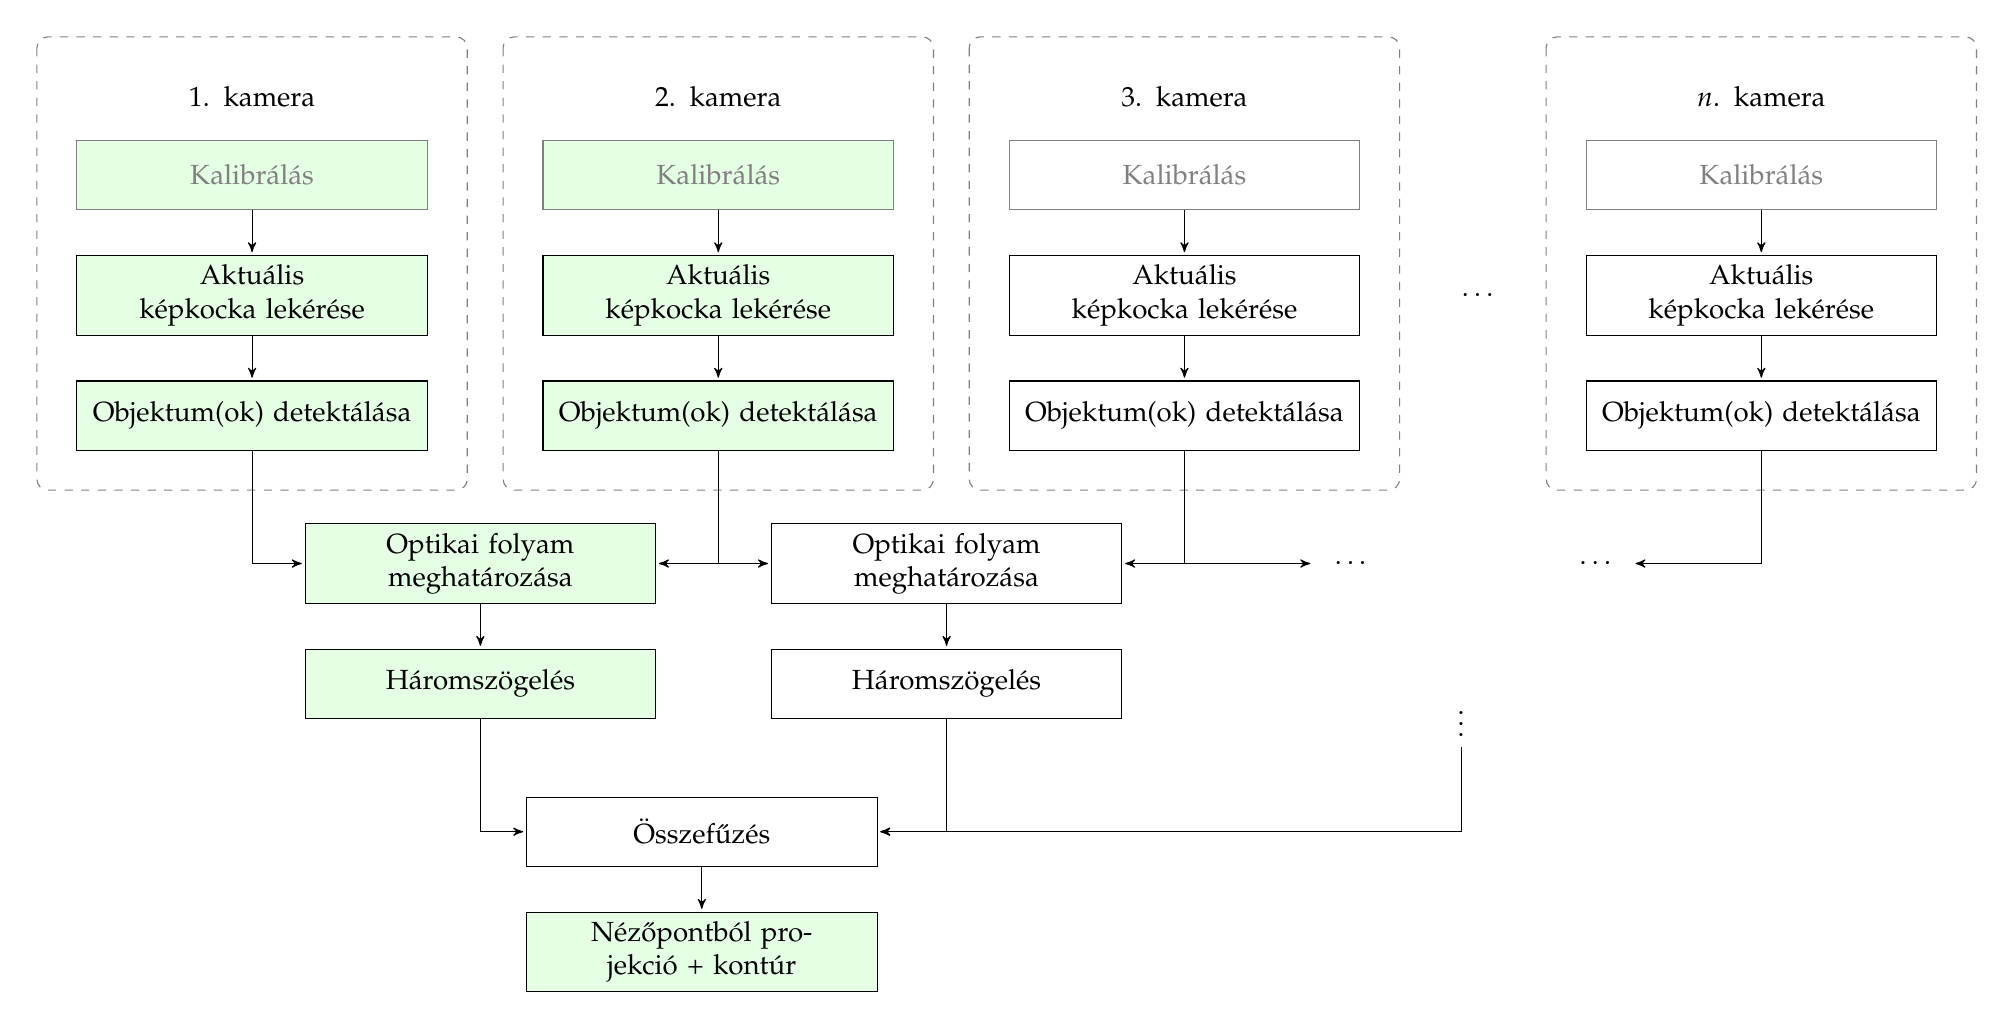
\begin{tikzpicture}[->,>=stealth',shorten >=1pt,auto]
\tikzset{
box/.style={draw, rectangle, text width=12em, minimum height=2.5em, text centered},
plain/.style={text width=12em, text centered},
line/.style = {-,shorten >=0pt},
graybox/.style = {box, gray}
}

\node[plain] (Cam1) {1. kamera};

\node[graybox,fill=green!10] (Calib1) [below of=Cam1] {Kalibrálás};

\node[box,fill=green!10] (GetFrames1) [below of=Calib1,yshift=-1.5em] {Aktuális képkocka lekérése};

\node[box,fill=green!10] (OD1) [below of=GetFrames1,yshift=-1.5em] {Objektum(ok) detektálása};

\draw (Calib1) -- (GetFrames1);
\draw (GetFrames1) -- (OD1);



\node[plain] (Cam2) [right of=Cam1,xshift=14em] {2. kamera};

\node[graybox,fill=green!10] (Calib2) [below of=Cam2] {Kalibrálás};

\node[box,fill=green!10] (GetFrames2) [below of=Calib2,yshift=-1.5em] {Aktuális képkocka lekérése};

\node[box,fill=green!10] (OD2) [below of=GetFrames2,yshift=-1.5em] {Objektum(ok) detektálása};

\draw (Calib2) -- (GetFrames2);
\draw (GetFrames2) -- (OD2);



\node[plain] (Cam3) [right of=Cam2,xshift=14em] {3. kamera};

\node[graybox] (Calib3) [below of=Cam3] {Kalibrálás};

\node[box] (GetFrames3) [below of=Calib3,yshift=-1.5em] {Aktuális képkocka lekérése};

\node[box] (OD3) [below of=GetFrames3,yshift=-1.5em] {Objektum(ok) detektálása};

\draw (Calib3) -- (GetFrames3);
\draw (GetFrames3) -- (OD3);



\node[plain] (CamN) [right of=Cam3,xshift=18em] {$n$. kamera};

\node[graybox] (CalibN) [below of=CamN] {Kalibrálás};

\node[box] (GetFramesN) [below of=CalibN,yshift=-1.5em] {Aktuális képkocka lekérése};

\node[box] (ODN) [below of=GetFramesN,yshift=-1.5em] {Objektum(ok) detektálása};

\draw (CalibN) -- (GetFramesN);
\draw (GetFramesN) -- (ODN);


\node[plain] (LDots) [right of=GetFrames3,xshift=7.75em] {$\ldots$};


\node[box,fill=green!10] (OF12) [below of=OD1,xshift=8.25em,yshift=-2.5em] {Optikai folyam meghatározása};
 
\draw (OD1) |- (OF12);
\draw (OD2) |- (OF12);


\node[box] (OF23) [below of=OD2,xshift=8.25em,yshift=-2.5em] {Optikai folyam meghatározása};
 
\draw (OD2) |- (OF23);
\draw (OD3) |- (OF23);


\node[plain] (OF34) [below of=OD3,xshift=6em,yshift=-2.5em,text width=2em] {$\ldots$};
\draw (OD3) |- (OF34);

\node[plain,below of=ODN,xshift=-6em,yshift=-2.5em,text width=2em] (OFnn) {$\ldots$};
\draw (ODN) |- (OFnn);



\node[box,fill=green!10] (Triangle12) [below of=OF12,yshift=-1.5em] {Háromszögelés};

\draw (OF12) -- (Triangle12);

\node[box] (Triangle23) [below of=OF23,yshift=-1.5em] {Háromszögelés};

\draw (OF23) -- (Triangle23);


\node[plain] (Others) [below of=OD3,xshift=10em,yshift=-8em,text width=2em] {$\vdots$};

\node[box] (Merge) [below of=Triangle12,xshift=8em,yshift=-2.5em] {Összefűzés};

\draw (Triangle12) |- (Merge);
\draw (Triangle23) |- (Merge);
\draw (Others) |- (Merge);


\node[box,fill=green!10] (Contour) [below of=Merge,yshift=-1.5em] {Nézőpontból projekció + kontúr};

\draw (Merge) -- (Contour);



\begin{pgfonlayer}{background}
    \path (Cam1.north west)+(-0.5,0.5) node (a) {};
    \path (OD1.south east)+(+0.5,-0.5) node (b) {};
    \path[rounded corners, draw=black!50, dashed] (a) rectangle (b);
\end{pgfonlayer}

\begin{pgfonlayer}{background}
    \path (Cam2.north west)+(-0.5,0.5) node (a) {};
    \path (OD2.south east)+(+0.5,-0.5) node (b) {};
    \path[rounded corners, draw=black!50, dashed] (a) rectangle (b);
\end{pgfonlayer}

\begin{pgfonlayer}{background}
    \path (Cam3.north west)+(-0.5,0.5) node (a) {};
    \path (OD3.south east)+(+0.5,-0.5) node (b) {};
    \path[rounded corners, draw=black!50, dashed] (a) rectangle (b);
\end{pgfonlayer}


\begin{pgfonlayer}{background}
    \path (CamN.north west)+(-0.5,0.5) node (a) {};
    \path (ODN.south east)+(+0.5,-0.5) node (b) {};
    \path[rounded corners, draw=black!50, dashed] (a) rectangle (b);
\end{pgfonlayer}

\end{tikzpicture}
}

\caption{Optikai folyamok módszere \label{fig:of-method}}
\end{sidewaysfigure}

Gondoljuk meg, hogy a fenti eljárás tetszőleges számú kamera-párra (amelyek nem feltétlen diszjunktak) általánosítható, és az így kapott pontfelhőket, felhasználva, hogy az adatokat az előzetes kalibrációnak köszönhetően egy közös világ-koordinátarendszerben kapjuk meg, ezeket könnyen egyesíthetjük. Ezt a folyamatot mutatja be \aref{fig:of-method}. ábra. A diplomaterv keretében a színezett hátterű lépések készültek el, a több kamerára vonatkozó együttes kezelés nem.

% --------------------------------
\section{Összefoglaló}
% --------------------------------

Ebben a fejezetben bemutattam az alkalmazott keretrendszert, melyre a megoldásomat építettem. Megfogalmaztam a célkitűzésem, miszerint két rögzített kamera által megfigyelt térrészben rekonstruálok egy illetve két mozgó objektumot egy a két kamera közötti szakaszon választott nézőpontból. Rögzítettem a sikerkritériumot, hogy a rekonstruálást akkor tekintem sikeresnek, ha a mozgó objektumok megközelítő kontúrjait sikeresen meghatározom. Végül leírtam az implementálásra kerülő rendszer lépésekre bontott logikáját.
    %----------------------------------------------------------------------------
\chapter{Megvalósítás}
%----------------------------------------------------------------------------

{\color{red} Először valami bla-bla}



%----------------------------------------------------------------------------
\section{Alapok}
%----------------------------------------------------------------------------



Az OpenCV remek keretrendszer, rengeteg gyakran használt algoritmust implementáltak benne, viszont felépítését tekintve procedurális. Jelen feladatom megoldása során törekedtem az átlátható és jól struktúrált kód kialakítására, így ahol szükségesnek éreztem osztályokba szerveztem a logikát.

OpenCV-ben a legtöbb adatot egy mátrix (\texttt{cv::Mat}) adattípus reprezentál, ide értve a matematikai értelemben vett mátrixokat és a képeket is. Egy ilyen mátrix lényegében egy kétdimenziós tömb, melynek elemei lehetnek skalárok, de több-dimenziós vektorok is (több csatornás).

Elsőnek a \texttt{Camera} osztály, és annak konkrét implementáció készültek el, elfedve azt, hogy éppen a valódi kamerából kérünk le képkockákat, vagy fájlból olvassuk ki azokat. Ebből adódóan a \texttt{RealCamera} lényegében becsomagolja az OpenCV-s \texttt{VideoCapture} osztályt, és a \texttt{Camera} absztakt osztály közös interfészt nyújt a fájlból történő olvasáshoz is a \texttt{FakeCamera} számára. Ez főleg a tesztelés során volt hasznos, hogy egy adott jelenetet elég volt egyszer felvenni, és utána azt tudtam bemenetként használni. Az osztálydiagram \aref{fig:cd:camera}. ábrán látható.

A \texttt{cameraMatrix} attribútum jelöli a \textit{kamera-mátrix}ot és a \texttt{distCoeffs} attribútum a torzítási együtthatókat (lásd \aref{sec:pinhole}. szekció). Mivel ezek egy kamerára nézve időben állandóak, ezért csak egyszer kell őket meghatározni. A \texttt{readCalibration()} metódus szolgál ezek külső fájlból történő beolvasásukra. Miután rendelkezésre állnak ezek a paraméterek, akkor a \texttt{readUndistorted()} metódus segítségével olvashatok be rektifikált képet. A másik 3 metódus megfelel az azonos nevű metódusoknak a \texttt{cv::VideoCapture} osztályban \cite{cv_video}, ahol a \texttt{grab()} egy képkockát szerez az eszköztől, de nem olvassa (dekódolja) ki, míg a \texttt{retrieve()} ezt teszi. Ezt a kombinációt több kamerás rendszernél célszerű használni, úgy, hogy először mindegyik kamerán meghívjuk a \texttt{grab()}-et, majd utána lekérjük a képeket (amely művelet időigényes). Ezzel a módszerrel érhető el, hogy időben a lehető legközelebb legyenek a különböző kamerákból lekért képkockák egymáshoz. A \texttt{read()} a kettőt kombinálja kényelmi szempontból.

\begin{figure}[tbh]
\centering

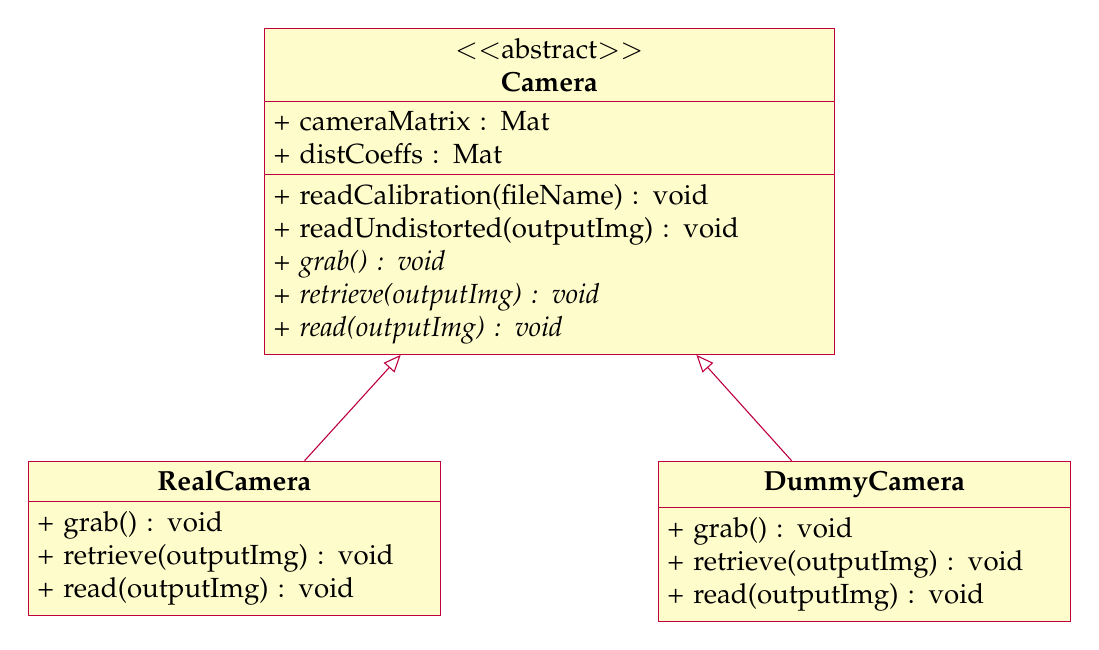
\begin{tikzpicture} 

\begin{abstractclass}[text width=7 cm]{Camera}{0, 0}
\attribute   {+ cameraMatrix : Mat}
\attribute   {+ distCoeffs : Mat}

\operation   {+ readCalibration(fileName) : void}
\operation   {+ readUndistorted(outputImg) : void}
\operation[0]{+ grab() : void}
\operation[0]{+ retrieve(outputImg) : void}
\operation[0]{+ read(outputImg) : void}
\end{abstractclass}

\begin{class}[text width=5 cm]{RealCamera}{-4, -5.5}
\inherit{Camera}
\operation{+ grab() : void}
\operation{+ retrieve(outputImg) : void}
\operation{+ read(outputImg) : void}
\end{class}

\begin{class}[text width=5 cm]{DummyCamera}{4, -5.5}
\inherit{Camera}
\operation{+ grab() : void}
\operation{+ retrieve(outputImg) : void}
\operation{+ read(outputImg) : void}
\end{class}

\end{tikzpicture}

\caption{Osztályok a kamerához kezeléséhez \label{fig:cd:camera}}
\end{figure}


\section{Kalibráció}

Elsőként meg kell határoznom a kamerák már előbb is említett belső paramétereit. A módszert \aref{sec:pinhole}. szekcióban mutattam be, a következőkben ennek megvalósítását tárgyalom. Ehhez készült egy segédosztály \texttt{Calibration} néven, melynek feladata, hogy kellő információ után meghatározza a kamera-mátrixot és a torzítási együtthatókat és kiírja ezeket egy fájlba, hogy azt vissza tudjuk olvasni.

\begin{figure}[tbh]
\centering

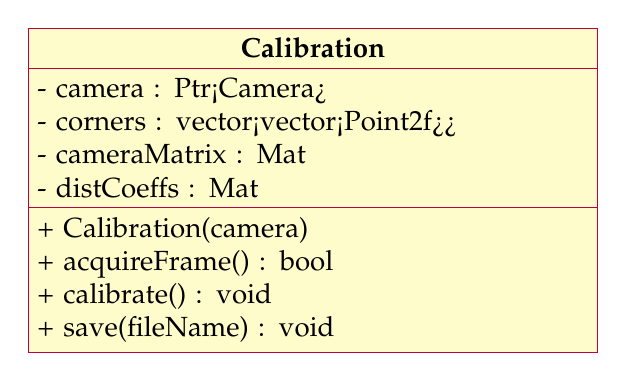
\begin{tikzpicture} 

\begin{class}[text width=7 cm]{Calibration}{0, 0}
\attribute{- camera : Ptr<Camera>}
\attribute{- corners : vector<vector<Point2f>{}>}
\attribute{- cameraMatrix : Mat}
\attribute{- distCoeffs : Mat}

\operation{+ Calibration(camera)}
\operation{+ acquireFrame() : bool}
\operation{+ calibrate() : void}
\operation{+ save(fileName) : void}
\end{class}

\end{tikzpicture}

\caption{\texttt{Calibration} osztály \label{fig:cd:calibration}}
\end{figure}

Konstruktorban át kell neki adni a kamerára vonatkozó pointert, amitől a képeket kell majd lekérnie. Az \texttt{acquireFrame()} metódus szerepe, hogy a kamera aktuális képkockáját megszerezze, megkeresse a képen a sakktáblát, és a sakktábla sarokponjaihoz tartozó koordinátákat a \texttt{corners} listához fűzze. Visszatérési értékben jelzi, hogy az adott képen sikeres volt-e a detekció. Belsőleg a \texttt{cv::findChessboardCorners()} OpenCV-s függvényt hívja, amelynek átadva egy fekete-fehér képet, megkapható a képen látható sakktábla sarokpontjainak képpontjai. Kellő képkocka után a \texttt{calibrate()} metódus segítségével a kérdéses két mátrix (\texttt{cameraMatrix}, \texttt{distCoeffs}) kiszámolható. Itt a \texttt{cv::calibrateCamera()} függvényt hívom segítségül, melynek két fontos bemeneti paraméterét emelem ki: az sarokpontok valóvilágbeli koordinátái, és a képeken detektált képpontjai sorfolytonosan (\texttt{corners}). A valóvilágbeli $(x, y, z)$ koordinátákat az egyszerűség kedvéért úgy választottam, hogy $z \equiv 0$, és $x$ valamint $y$ egész számok úgy, hogy a sakktábla bal felső sarka $(0, 0, 0)$, jobb alsó sarka pedig -- $9\times 6$-os sakktáblát használva -- $(9, 6, 0)$. A \texttt{save()} pedig kimenti a paramétereket olyan formátumban, amiből a \texttt{Camera::readCalibration()} vissza tudja olvasni.


\subsection{Kamerák pozíciójának meghatározása világkoordinátákban}


Rögzített kamerák révén lehetőségem adódik, hogy előre meghatározzam a kamerák pozícióját és nézőpontjuk irányát. Erre egy kalibrációs objektumot használok, szintén egy sakktáblát. Amennyiben megadom a sakktábla sarokpontjainak koordinátáit az előbbiekkel egyező módon, akkor a sakktábla rögzítésével a térben, a koordinátarendszert is rögzítem. 

Az OpenCV-ben erre a célra van a \texttt{solvePnP} függvény, mely 3D-2D pont-összerendelésekből, kiszámolja a forgatási és eltolási vektort, amik együttesen megadják a transzformációt a model-koordinátarendszerből a kamera koordinátarendszerébe. Ezen funkciót a \texttt{CameraPoseCalculator} osztály ágyazza be, és a két vektort pedig a \texttt{CameraPose} csomagolja össze egy perzisztálható osztályba, lásd \aref{fig:cd:pose}. ábra.

\begin{figure}[tbh]
\centering

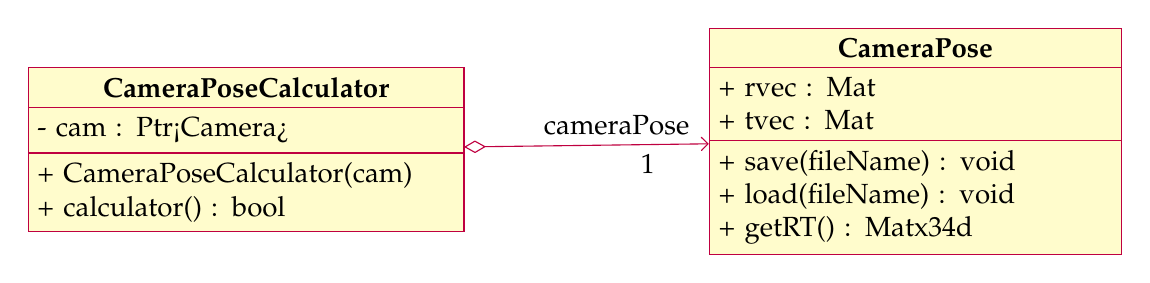
\begin{tikzpicture} 

\begin{class}[text width=5.3 cm]{CameraPoseCalculator}{-8.5, -0.50}
\attribute{- cam : Ptr<Camera>}

\operation{+ CameraPoseCalculator(cam)}
\operation{+ calculator() : bool}
\end{class}

\begin{class}[text width=5 cm]{CameraPose}{0, 0}
\attribute{+ rvec : Mat}
\attribute{+ tvec : Mat}

\operation{+ save(fileName) : void}
\operation{+ load(fileName) : void}
\operation{+ getRT() : Matx34d}
\end{class}

\aggregation{CameraPoseCalculator}{cameraPose~~~~~~~~~~}{1}{CameraPose}

\end{tikzpicture}

\caption{\texttt{CameraPoseCalculator} és \texttt{CameraPose} osztály \label{fig:cd:pose}}
\end{figure}

A \texttt{CameraPoseCalculator} osztály megkapja konstruktor argumentumaként annak a kamerára mutató pointerét, amelynek a külső paramétereit (forgatási és eltolási vektor, lásd \ref{sec:pinhole}. szekció vége) ki kell számolnia. A konkrét művelet végrehajtásáért a \texttt{calculator()} metódus felelős, amely a kamerától lekér egy képkockát, megkeresi rajta a sakktáblát, majd meghívja a \texttt{cv::solvePnP()} függvényt. Visszatérési értékben jelzi, hogy sikeres volt-e a detekció, ha igen, akkor lekérhető tőle a \texttt{CameraPose} példány. Ez utóbbi a \texttt{save()} és \texttt{load()} metódusokkal elmenthető és visszatölthető, így ameddig a kamerát nem mozgatjuk el, ez újra felhasználható. A \texttt{getRT()} metódus a forgatási vektorból forgatási mátrixot csinál (Rodrigues-féle forgatási formula \cite{camera-calib-3d}) és összefűzi azt az eltolási vektorral egy $3\times 4$-es $\Big(\,\mathbf{R}\,|\,\mathbf{t}\,\Big)$ forgatás-eltolás mátrixba.

A kamera külső paramétereinek meghatározása után már minden információ adott, hogy 3D-s pontok 2D-s vetületeit meg tudjam határozni a \texttt{cv::projectPoints()} függvény felhasználásával. \Aref{fig:pose}. ábrán látható, hogy egy a sakktábla síkjába rajzolt négyzetrács, melynek egyik jelölt pontja a világ-koordinátarendszer origója.

\begin{figure}[tbh]
\centering
\begin{subfigure}[b]{.49\linewidth}
	\centering
	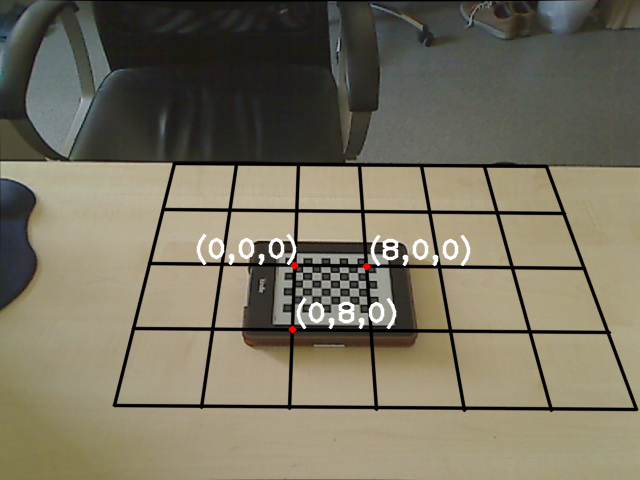
\includegraphics[width=205pt]{figures/pose0_180.png}
	\caption{Bal oldali kamera}
  \end{subfigure}
\begin{subfigure}[b]{.49\linewidth}
	\centering
	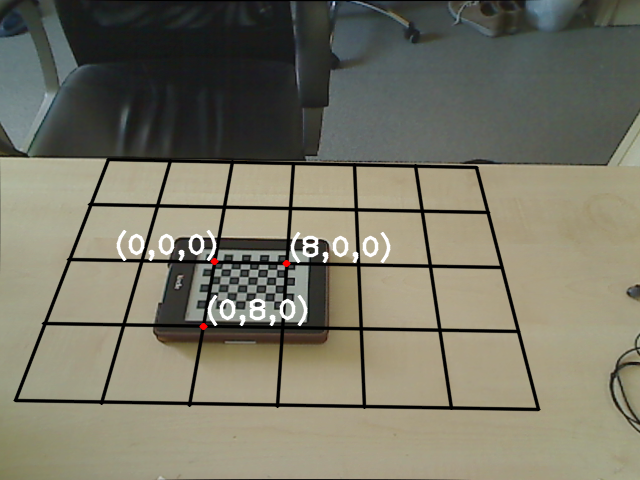
\includegraphics[width=205pt]{figures/pose1_180.png}
	\caption{Jobb oldali kamera}
  \end{subfigure}
\caption{Világ-koordinátarendszer jelölése a képeken \label{fig:pose}}
\end{figure}

%----------------------------------------------------------------------------
\section{Objektum detekció}
%----------------------------------------------------------------------------

A következőkben az objekumok detekciójáról lesz szó. Először bemutatok két megközelítést az előtér maszk meghatározásához, ami lényegében a két képen kijelöli a mozgó részek maszkját. Ezt követően a maszkokat szegmentálni kell különálló \textit{blob}okra, és ezeket a két képen egymásnak megfeleltetni, hogy megkapjuk egy objektum két maszkját.

    %----------------------------------------------------------------------------
    \subsection{Előtér maszk meghatározása}
    %----------------------------------------------------------------------------


\subsubsection{Előtér-háttér szegmentáció}

\Aref{sec:obj_detection}. szekcióban leírtam a mozgó objektumok detekciójának egy lehetséges megközelítését. A lényege, hogy egy háttér modellt építünk, és így mindig aktuálisan lekérhető az előtérhez tartozó maszk, ami kijelöli a mozgó objektumokat. A probléma megoldása két fázisra bontható: először egyetlen objektumot keresek és detektálok, majd később több mozgó objektumot is.

Mindkét fázisnak közös része a már említett modellépítés, melyhez az OpenCV-ben megtalálható \texttt{BackgroundSubtractorMOG2} osztályt \cite{opencv-mog} hívom segítségül. Példányosítás után a modell építése, és az aktuális maszk kinyerése az \texttt{apply} metódussal történik. \Aref{fig:my_mog2}. ábrán látható a kinyerhető maszkra egy példa.

\begin{figure}[tbh]
\centering
\begin{subfigure}[b]{.32\linewidth}
	\centering
	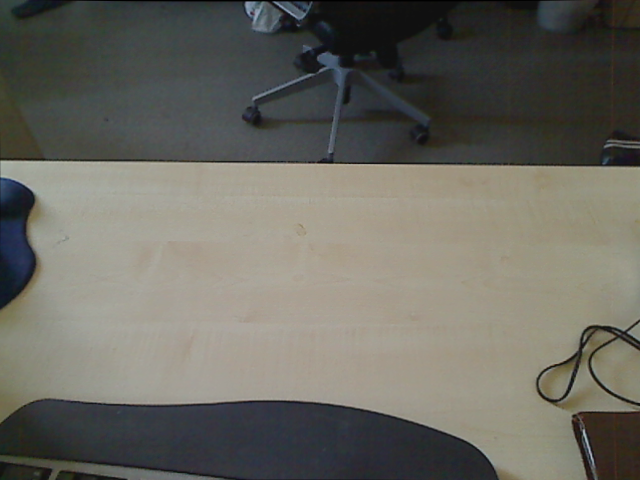
\includegraphics[width=137pt]{figures/image230.png}
	\caption{Statikus kép -- ,,háttér''}
  \end{subfigure}
\begin{subfigure}[b]{.32\linewidth}
	\centering
	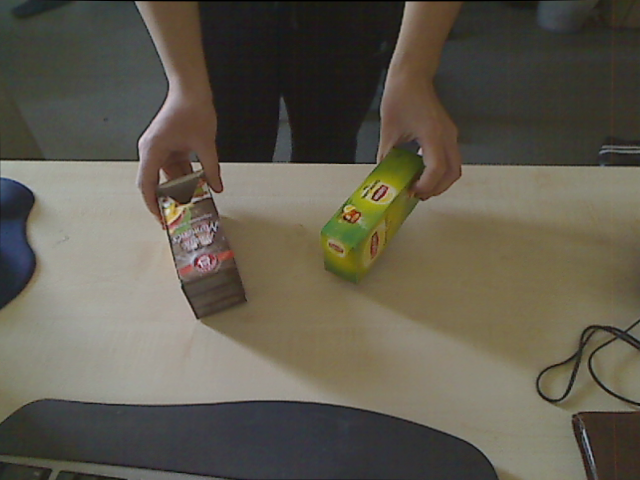
\includegraphics[width=137pt]{figures/image343.png}
	\caption{Mozgó képsor egy képe}
  \end{subfigure}
\begin{subfigure}[b]{.32\linewidth}
	\centering
	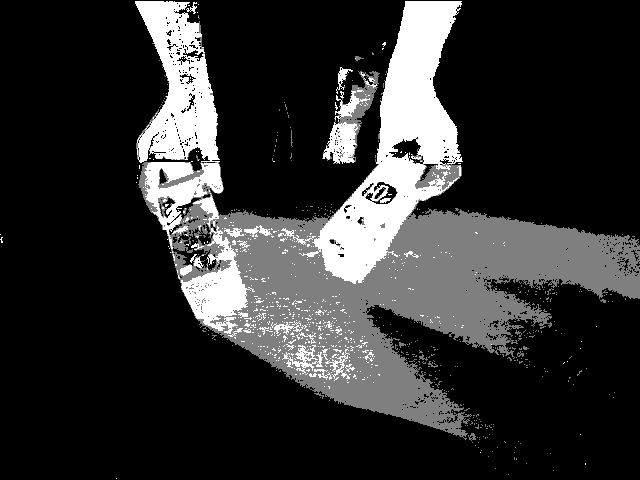
\includegraphics[width=137pt]{figures/mask343.png}
	\caption{Kapott előtér maszk}
  \end{subfigure}
\caption{Példa az előtér maszkra \label{fig:my_mog2}}
\end{figure}

Megfigyelhető, hogy a maszk nem pusztán bináris, hanem azt is jelzi, amit az algoritmus árnyéknak gondol. A zajt a maszkon az erózió-dilatáció morfológiai módszerek segítségével tudjuk csökkenteni. Előbbi a kisméretű zajokat tünteti el, utóbbi pedig a lyukakat szünteti meg. OpenCV-ben ezek implementációi a \texttt{dilate} és \texttt{erode} függvények. Előbbi az adott pixelt a környezetében (amit egy kernel ír le) lévő maximális, míg utóbbi a minimális értékkel helyettesít. Én egy erózió-dilatáció-erózió lépéssorozatot használok: először az apróbb szemcsék szűnnek meg, utána a lyukak. Az utolsó erózió szerepe, hogy az objektumok szélén a dilatáció miatt jelentkező növekedést megszűntesse. Ennek eredménye látható \aref{fig:erosion_dilation}. ábrán.

\begin{figure}[tbh]
\centering
\begin{subfigure}[b]{.49\linewidth}
	\centering
	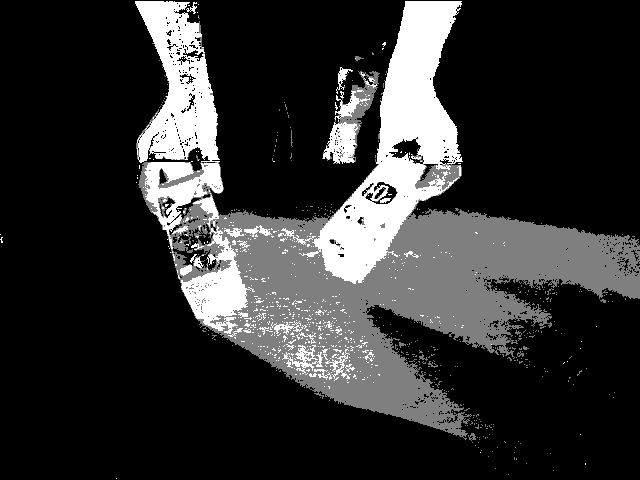
\includegraphics[width=205pt]{figures/mask343.png}
	\caption{Eredeti}
  \end{subfigure}
\begin{subfigure}[b]{.49\linewidth}
	\centering
	
\includegraphics[width=205pt]{figures/mask343_fixed.png}
	\caption{Árnyékok kivétele és zajcsökkentés után}
  \end{subfigure}
\caption{Előtér maszk zajmentesítése \label{fig:erosion_dilation}}
\end{figure}

Megfigyelhető, hogy a bal oldali dobozhoz tartozó maszk része annyira zajos volt, hogy a nagy lyuk nem szűnt meg, míg a kevésbé zajos jobb oldali doboz rendben megmaradt. A maszkot alkalmazva az eredeti képre \aref{fig:mask_applied}. ábrán látható, hogy egy bizonyos hibahatáron belül sikeresnek tekinthető a mozgó részlet kijelölése.

\begin{figure}[tbh]
\centering
\begin{subfigure}[b]{.49\linewidth}
	\centering
	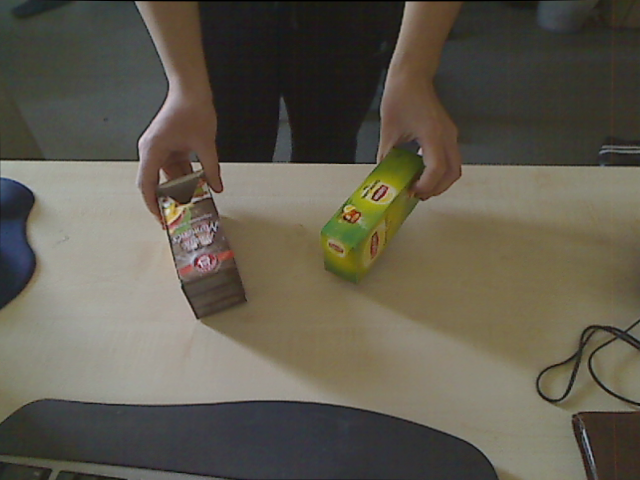
\includegraphics[width=205pt]{figures/image343.png}
	\caption{Eredeti kép}
  \end{subfigure}
\begin{subfigure}[b]{.49\linewidth}
	\centering
	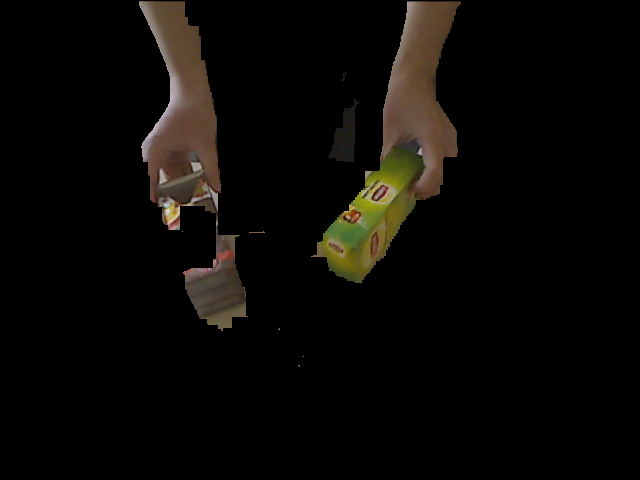
\includegraphics[width=205pt]{figures/mask343_applied.png}
	\caption{A detektált előtér}
  \end{subfigure}
\caption{Előtér maszk alkalmazás az eredeti képre \label{fig:mask_applied}}
\end{figure}

    %----------------------------------------------------------------------------
    \subsubsection{Előtér meghatározása optikai folyamokkal}
    %----------------------------------------------------------------------------
    
Másik megközelítésem, hogy már az előtér meghatározásához is az optikai folyamokat hívom segítségül. 

\Aref{chapter2}. fejezetben bemutattam a sűrű optikai folyamok meghatározására Gunner Farnebäck módszerét. OpenCV-ben ezt a \texttt{cv::calcOpticalFlowFarneback()} \cite{opencv-mog} függvény valósítja meg. Az algoritmus szempontjából fontos paraméterei közül kiemelnék párat:

\begin{enumerate}
\item \texttt{pyr\_scale} -- a már említett piramis-módszerhez kapcsolódó paraméter: azt definiálja, hogy rétegenként a következő réteg hányszorosa az előzőnek (ennek segítségével a nagy elmozdulások kisebbek lesznek a kisebb rétegeken)
\item \texttt{levels} -- piramis rétegeinek a száma, 1-nél csak az eredeti képet használja, továbbiak nélkül
\item \texttt{winsize} -- az ablak méret, amit a mintavételezéshez használ
\item \texttt{iterations} -- iterációk száma minden piramis rétegen
\end{enumerate}

Tekintve, hogy nekünk csak az a fontos, hogy a lehető leggyorsabban kapjunk elmozdulásvektorokat, a paramétereket a következőknek megfelelően állítottam be: ne építsünk piramist (\texttt{levels = 1}, így \texttt{pyr\_scale} beállítása lényegtelen), valamint kicsit ablakmérettel dolgozzunk ($3\times 3$, tehát \texttt{winsize = 3}), valamint rétegenként elég 1 iteráció (\texttt{iterations = 1}).

A kiszámolt vektormezőből pedig a maszkot úgy határozom meg, hogy minden, egységnél hosszabb (tehát legalább 1 pixelnyi a becsült mozgása) vektor végpontját megjelölöm. Ezáltal lényegében azon részeket határoztam meg, ahova éppen a pontok mozdultak, ez pedig pontosan azon részei a képnek, ahol az adott képkockán az előtérben mozgó objektumokat éppen várjuk. Az előzőekhez hasonlóan a maszkon itt is végzünk apró utófeldolgozást a dilatáció és erózió morfológiai műveletek segítségével. Az eredményt \aref{fig:of_mask}. ábra mutatja be. Megfigyelhető, hogy a jól textúrázott objektumokhoz nagyon jó maszkot kapunk, a textúrázatlan területeken pedig a pontokat úgy tekinti mintha statikusak lennének.

\begin{figure}[tbh]
\centering
\begin{subfigure}[b]{.32\linewidth}
	\centering
	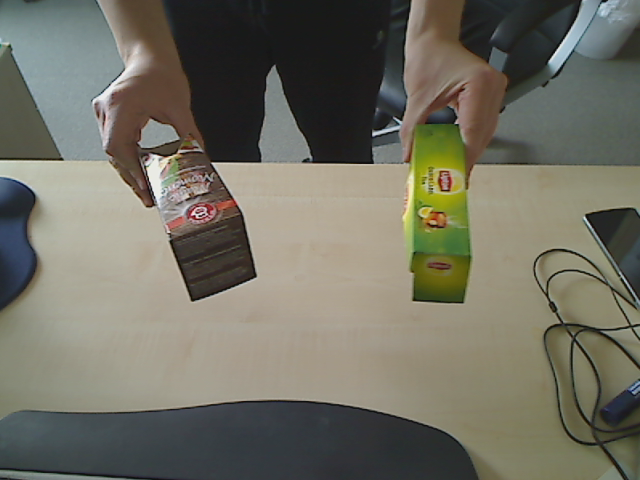
\includegraphics[width=137pt]{figures/frame_ofmask_101.png}
	\caption{2. képkocka}
  \end{subfigure}
\begin{subfigure}[b]{.32\linewidth}
	\centering
	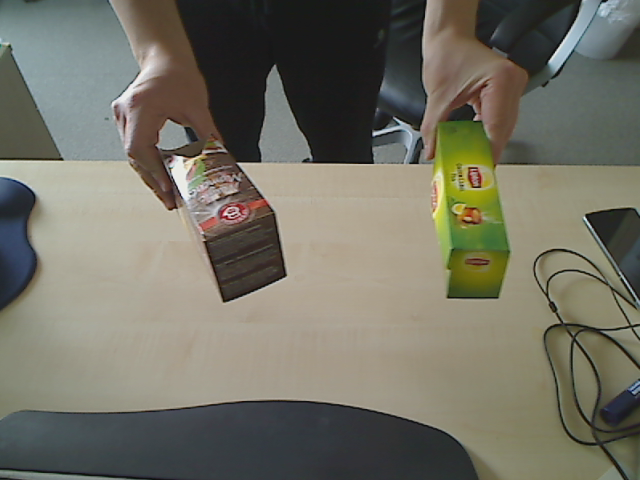
\includegraphics[width=137pt]{figures/frame_ofmask_104.png}
	\caption{3. képkocka}
  \end{subfigure}
\begin{subfigure}[b]{.32\linewidth}
	\centering
	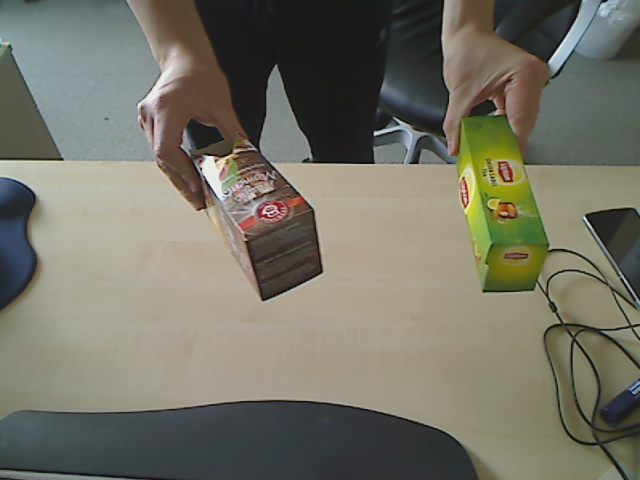
\includegraphics[width=137pt]{figures/frame_ofmask_107.png}
	\caption{4. képkocka}
  \end{subfigure}\\
\begin{subfigure}[b]{.32\linewidth}
	\centering
	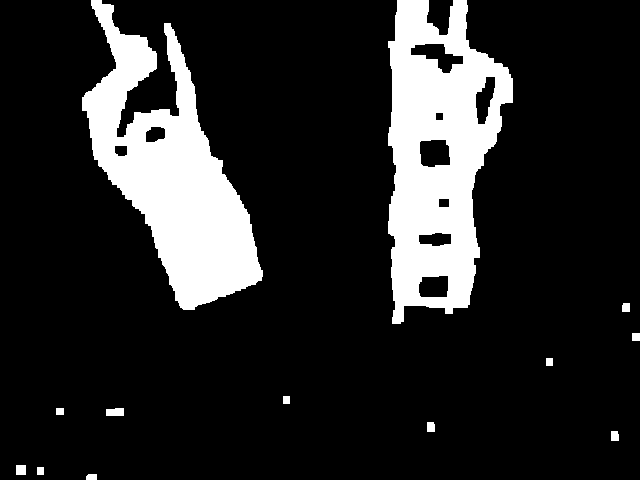
\includegraphics[width=137pt]{figures/mask_ofmask_101.png}
	\caption{2. maszk}
  \end{subfigure}
\begin{subfigure}[b]{.32\linewidth}
	\centering
	
\includegraphics[width=137pt]{figures/mask_ofmask_104.png}
	\caption{3. maszk}
  \end{subfigure}
\begin{subfigure}[b]{.32\linewidth}
	\centering
	
\includegraphics[width=137pt]{figures/mask_ofmask_107.png}
	\caption{4. maszk}
  \end{subfigure}
\caption{Egy jelenet 3 képkockája és ezekből az optikai folyamok felhaszánlásával kapott maszkok (már zajcsökkentés után) \label{fig:of_mask}}
\end{figure}


Az osztálydiagramot \aref{fig:cd:fg-mask-calc}. ábra mutatja be. \texttt{ForegroundMaskCalculator} osztály lényegében egy közös interfészt nyújt csak, valamint egy \texttt{morph()} metódust tartalmaz, mely a morfológiai műveleteket végzi el a maszkon. A \texttt{MOG2ForegroundMaskCalculator} az OpenCV-s \texttt{BackgroundSubtractorMOG2} osztály egy példányát csomagolja be, ami minden új képkockát megkap, és visszaadja a maszkot, az algoritmus által árnyéknak jelölt részeket a \texttt{removeShadows()} távolítja el. \texttt{OFForegroundMaskCalculator} pedig eltárolja az előző képkockát, és ebből meg az éppen aktuális képkockából \texttt{calcOpticalFlowFarneback()} segítségével a lehető leggyorsabban meghatározza a képkockákra az optikai folyamot, melyből aztán az előbbiekben ismertetett módszerrel a \texttt{getMaskFromFlow()} adja vissza a maszkot.

\begin{figure}[tbh]
\centering

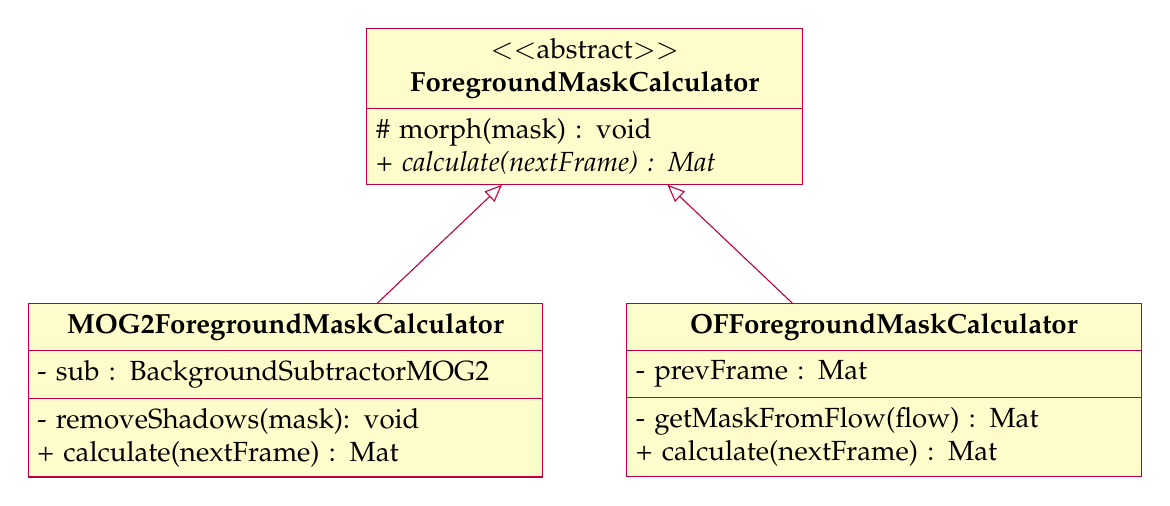
\begin{tikzpicture} 

\begin{abstractclass}[text width=5.3 cm]{ForegroundMaskCalculator}{0, 0}

\operation   {\# morph(mask) : void}
\operation[0]{+ calculate(nextFrame) : Mat}

\end{abstractclass}

\begin{class}[text width=6.3 cm]{MOG2ForegroundMaskCalculator}{-3.8, -3.5}
\inherit{ForegroundMaskCalculator}
\attribute{- sub : BackgroundSubtractorMOG2}
\operation{- removeShadows(mask): void}

\operation{+ calculate(nextFrame) : Mat}
\end{class}

\begin{class}[text width=6.3 cm]{OFForegroundMaskCalculator}{3.8, -3.5}
\inherit{ForegroundMaskCalculator}
\attribute{- prevFrame : Mat}
\operation{- getMaskFromFlow(flow) : Mat}

\operation{+ calculate(nextFrame) : Mat}
\end{class}

\end{tikzpicture}

\caption{Előtér maszk meghatározására szolgáló implementációk \label{fig:cd:fg-mask-calc}}
\end{figure}

%----------------------------------------------------------------------------
\subsection{Egyetlen objektum detekciója}
%----------------------------------------------------------------------------

Kezdetben azzal az egyszerűsítéssel élek, hogy a képen csak egyetlen mozgó objektumot detektálok, mégpedig azt, amelyik a legnagyobb részt foglalja el a képeken. Ez nagyban egyszerűsíti a dolgokat, mert ahogy majd látni fogjuk a következő szekcióban, az optikai folyam meghatározására szükség lesz a képeken látható \textit{blob}ok (egy objektumhoz tartozó egybefüggő rész a képen) párosításra a kamerák képein. Mivel összesen egy blobot jelölök ki a képeken, ezek párosítása triviális, és nagy valószínűséggel ugyanazon objektumhoz tartoznak majd.

Ehhez először szükség van az összefüggő komponensek kiválasztására. Két módszer kínálkozik erre OpenCV-ben; az egyik a \texttt{findContours()} függvény, ami megkeresi a képen látható kontúrokat (paraméterezhető, hogy csak a legkülsőbbeket találja meg, a belső kontúrokat nem), a másik pedig a a \texttt{connectedComponentsWithStats()}, mely a 3.0-s verziótól érhető el. Az első abban különbözik az utóbbitól, hogy a kapott kontúrt felhasználva megkaphatjuk a belső területet (lyukak nélkül), míg utóbbi lényegében a maszk pixeleit címkézi fel, hogy melyik komponenshez tartoznak. Ezért én az előbbi használata mellett döntöttem. Miután megvannak ezek a kontúrok a belső területeket meghatározom a \texttt{cv::contourArea()} függvénnyel, és egy maximum kiválasztás után megkapom a legnagyobb területtel rendelkező komponens maszkjával. Mindkét képre elvégezve ezt, megkapom az egyik és másik képen a legnagyobb objektumhoz tartozó 1-1 maszkot. Az algoritmus eredmény \aref{fig:single-obj}. ábrán látható.

\begin{figure}[tbh]
\centering
\begin{subfigure}[b]{.49\linewidth}
	\centering
	
\includegraphics[width=205pt]{figures/mask_ofmask_104.png}
	\caption{Eredeti maszk}
  \end{subfigure}
\begin{subfigure}[b]{.49\linewidth}
	\centering
	
\includegraphics[width=205pt]{figures/mask_ofmask_104_selected.png}
	\caption{Detektált blobok, és fehérrel a legnagyobb}
  \end{subfigure}
\caption{Legnagyobb területű blob kijelölése \label{fig:single-obj}}
\end{figure}

%----------------------------------------------------------------------------
\subsection{Több objektum detekciója, párosítás a kamerák képein}
%----------------------------------------------------------------------------

A következő feladat, amit meg kell oldanom, az több objektum együttes detekciója, úgy, hogy a két képen az egymásnak megfelelő blobokat párosítsam. Ehhez jellegzetes pontokat, és ezekhez tartozó leírókat keresek, illetve számolok ki a képi információkból.

A szakirodalomban több algoritmust is találhatunk, mely vagy a jellegzetes pontok (\textit{feature}) detektálásában (pl. FAST \cite{FAST}, MSER \cite{MSER}), vagy ezen pontokhoz tartozó leírók (\textit{feature descriptor}) kinyerésében (pl. FREAK \cite{FREAK}), vagy mindkettőre használhatóak (pl. ORB \cite{ORB}, SIFT \cite{SIFT} és SURF \cite{SURF}). SIFT és a SURF a tradícionális leírók közé sorolhatóak abban a tekintetben, hogy vektor-alapú leírokat készítenek, ellenben az újabbakkal, amelyek bináris-füzéreket. Előbbi algoritmusok kiszámolása idő- és erőforrásigényes, valós idejű, valamint mobil eszközökön történő alkalmazásra nem alkalmasak, ellenben utóbbiak igen, és a kinyert leírók összehasonlítása is gyors (Hamming-távolság). Dolgozatomnak nem célja ezek mélgyreható vizsgálata és rangsorolása, de \cite{feature-detection-comparison} alapján a FAST-ot választottam detekcióhoz és a FREAK-et a leírók kinyeréséhez, mert \cite{FREAK}-ben meggyőzőek voltak az eredmények.

Miután mindkét képen megkerestem a jellegzetes pontjaikat, és kinyertem hozzájuk a leírókat, ezeket párosítani kell. Ehhez használhatunk brute-force módszert (mindent mindennel összehasonlítva és kiválasztva a legközelebbit), vagy a FLANN (Fast Approximate Nearest Neighbor Search Library \cite{flann_pami_2014}) könyvtárat, melyhez OpenCV-ben is elkészült az interfész \cite{opencv-flann}. Ez első sorban arra használható, hogy gyorsan tudjunk több dimenziós vektortérben egy vektorhoz megkeresni a hozzá legközelebbi vektort, amely SIFT és SURF esetben ideális, de használható bináris leírókhoz is \cite{flann-binary}. Mivel a halmaz mérete, ahol a párosítást keressük, nem olyan nagy, hogy a brute-force módszer hátránya kiütközzön, ezért emellett maradtam, melynek OpenCV-ben az implementációját a \texttt{cv::BFMatcher} osztályban találjuk.

Végül a kapott párosításokat a fundamentális mátrix segítségével validálom és kiszűröm, vagyis megnézem, hogy a már használt epipoláris ($\mathbf{u}'^T \mathbf{F} \mathbf{u} = 0$) kényszer egy adott hibahatáron belül teljesül-e. Gondoljuk meg, hogy ettől még maradhat teljesen rossz párosítás is a halmazban, hiszen az adott ponthoz csak azt nézi meg, hogy a másik pont rajta van-e a hozzá tartozó epipoláris egyenesen. \Aref{fig:multi-obj-matches}. ábrán látható néhány találat. {\color{red}Megfigyelhető, hogy van olyan egyezőség, amely ugyanazon ismétlődő motívum (teás doboz logója a bal oldali képen) egy részét találta meg két különböző helyen a dobozon, valamint, hogy talál egyezőséget a két doboz között is.}

\begin{figure}[tbh]
\centering
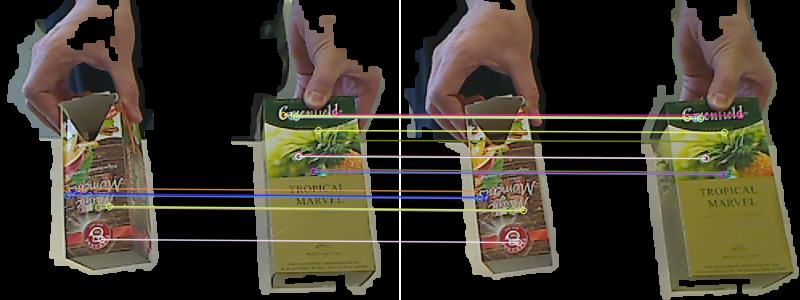
\includegraphics[width=400pt]{figures/multi_obj_matches.png}
\caption{\color{red} REGGEL JOBBAT!!! RÁZZOMOLVA! Blobok által kijelölt képrészleteken az egymásnak megfelelő pontok keresése (29 találat) \label{fig:multi-obj-matches}}
\end{figure}

Ezt követően a blobokat a következőképpen párosítom. Veszem azt a képet, amelyiken több blob van, mint a másikon (ha ugyanannyi, akkor a választás tetszőleges), majd egyesével az itt lévő blobokhoz megkeresem, hogy a benne lévő párosításbeli pontok párjainak többségét melyik másik képen lévő blob tartalmazza. Így kapok egy projekciót a több elemű halmazból a kisebbe. Nem feltétlen lesz minden blobnak párja (nem tartalmaz \textit{feature} pontot), valamint lehet, hogy több különböző blob is ugyanahhoz a blobhoz fog tartozni, ekkor ezeket összevonom egy blobbá. Így a végén a blobok egy részhalmazához egy kölcsönösen egyértelmű relációt, párosítást kapok, ezek jelölik ugyanazon objektum két maszkját a két képen. {\color{red}Párosításért lásd... ábra}

Annak érdekében, hogy a következő lépéseket könnyebben tudjam tesztelni, aktívan fogom használni a csak egy objektum detekciójára képes algoritmust is, ezért a két megoldásnak interoperábilisnak kell lennie. Tehát mindkettő egy közös \texttt{ObjectSelector} absztrakt osztályból származik, lásd \ref{fig:cd:objectselector}. ábra. Későbbiekben fogjuk látni, hogy ennél a módszernél is jó, ha meghatározzuk az egymásnak megfelelő pontokat, így végülis mindkettő megkapja konstruktorában a \texttt{Matcher} osztály egy példányát, melyet a \texttt{ObjectSelector} őriz. A \texttt{Matcher} két képkockából és az előtér maszkokból meghatározza az egymásnak megfelelő pontokat, melyeket pontpáros listájaként ad vissza. Konstruktorában azért, hogy a találatokat szűrni tudja megkapja a kamera objektumokat és a fundamentális mátrixot. Mindkét konkrét \texttt{ObjectSelector} megvalósítás \texttt{Object} listával tér vissza, mely tartalmazza a két maszkot a két képen, valamint az összetartozó pontokat.


\begin{figure}[tbh]
\centering

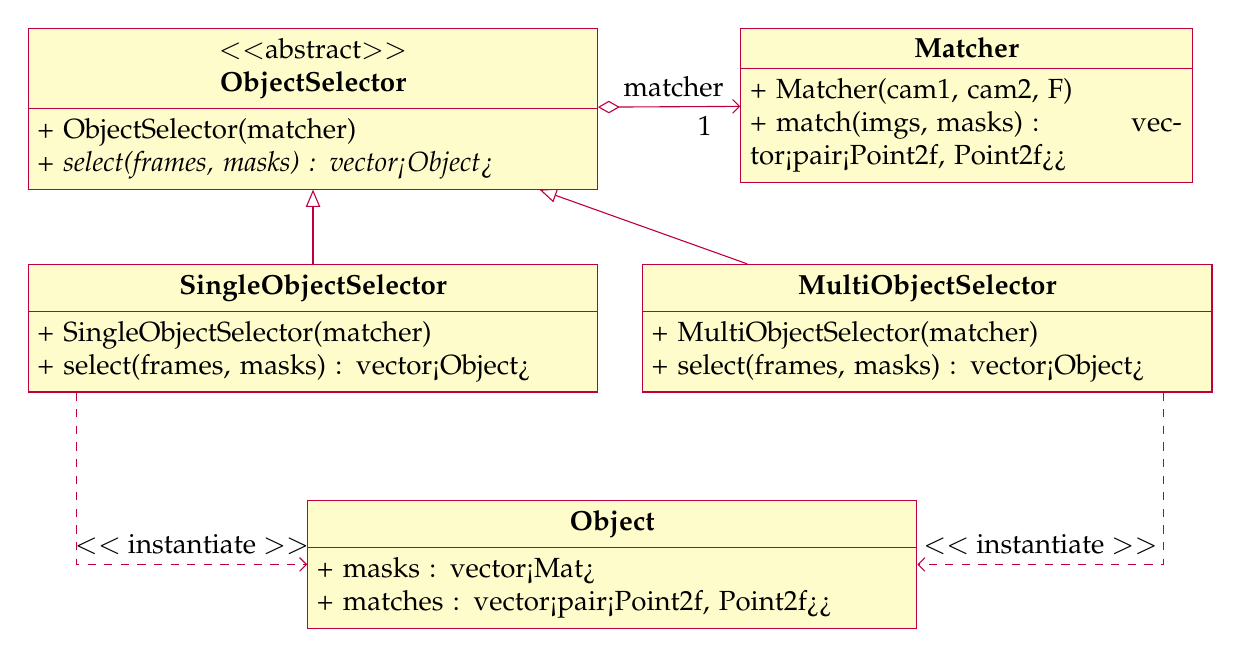
\begin{tikzpicture} 

\begin{class}[text width=5.5 cm]{Matcher}{4.5, 0}

\operation{+ Matcher(cam1, cam2, F)}
\operation{+ match(imgs, masks) : ~~~~~~~ vector<pair<Point2f, Point2f>{}>}

\end{class}

\begin{abstractclass}[text width=7 cm]{ObjectSelector}{-3.8, 0}

\operation   {+ ObjectSelector(matcher)}
\operation[0]{+ select(frames, masks) : vector<Object>}

\end{abstractclass}


\aggregation{ObjectSelector}{matcher~~~~~~~~~~}{1}{Matcher}


\begin{class}[text width=7 cm]{SingleObjectSelector}{-3.8, -3}
\inherit{ObjectSelector}

\operation{+ SingleObjectSelector(matcher)}
\operation{+ select(frames, masks) : vector<Object>}
\end{class}

\begin{class}[text width=7 cm]{MultiObjectSelector}{4, -3}
\inherit{ObjectSelector}

\operation{+ MultiObjectSelector(matcher)}
\operation{+ select(frames, masks) : vector<Object>}
\end{class}

\begin{class}[text width=7.5 cm]{Object}{0, -6}
\operation{+ masks : vector<Mat>}
\operation{+ matches : vector<pair<Point2f, Point2f>{}>}
\end{class}

\draw[umlcd style dashed line,->] (SingleObjectSelector.south) ++
(-3,0) |- node [above,sloped,black,pos=0.75]{$ < <$ instantiate $ > >$} (Object);

\draw[umlcd style dashed line,->] (MultiObjectSelector.south) ++
(3,0) |- node [above,sloped,black,pos=0.75]{$ < <$ instantiate $ > >$} (Object);

\end{tikzpicture}

\caption{Objektumok kijelölését szolgáló osztályok \label{fig:cd:objectselector}}
\end{figure}



%----------------------------------------------------------------------------
\section{Optikai folyam meghatározása}
%----------------------------------------------------------------------------

{\color{red} Kicsit átírni...}

\Aref{chapter2}. fejezetben bemutattam a sűrű optikai folyamok meghatározására Gunner Farnebäck módszerét. Ennek alkalmazását, valamint OpenCV-ben történő implementációjáról lesz szó ebben a részben.

A \texttt{cv::calcOpticalFlowFarneback()} függvény segítségével két képkockán meghatározhatom az optikai folyamot. Az algoritmus jellegéből adódóan nagy mozgásokat nem tud követni, de az implementáció támogatja a piramis-módszert, azaz nagy mozgások esetén a képeket több lépcsőben kicsinyíti, így az eredeti képen lévő nagy mozgások kisebbek lesznek, a kicsik pedig eltűnnek. A futási idő természetesen függ a kép méretétől, így fontos, hogy kihasználjuk az objektum maszkjából nyerhető információt.

A következőkben \aref{fig:of_original}. ábrán látható két képkocka lesz a kiinduló állapot, már az előbbiekben bemutatott előtér maszk által kijelölve. A képkockák két olyan kamera beállításal készültek, ahol a két kamera képsíkja nagyjából egybe esik (egy irányba néznek), és csak víszintes irányban vannak egymáshoz képest eltolva.

\begin{figure}[tbh]
\centering
\begin{subfigure}[b]{.49\linewidth}
	\centering
	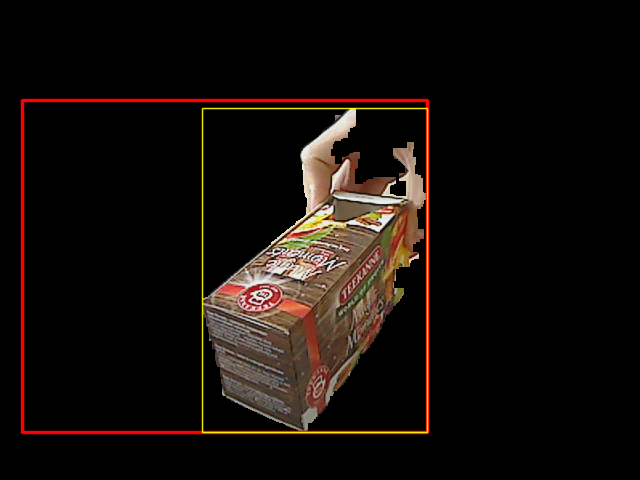
\includegraphics[width=205pt]{figures/of_img_left_framed.png}
  \end{subfigure}
\begin{subfigure}[b]{.49\linewidth}
	\centering
	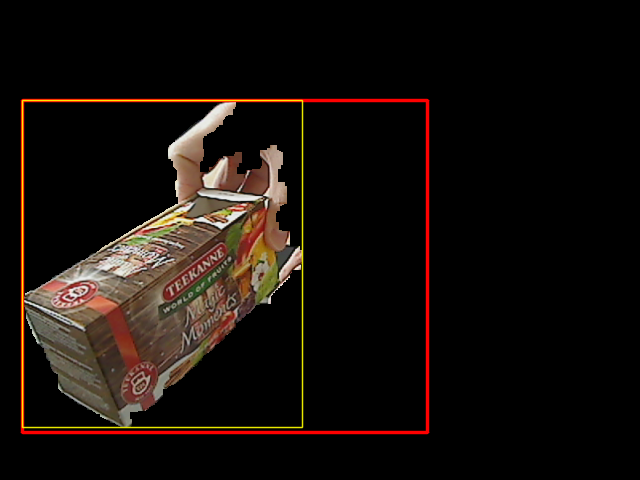
\includegraphics[width=205pt]{figures/of_img_right_framed.png}
  \end{subfigure}
\caption{Bal és jobb kamera által látott objektum kijelölve; a sárga keretek jelölik az objektumok befoglaló téglalapjait, a piros pedig ezen téglalapokat tartalmazó legkisebb területű téglalapot \label{fig:of_original}}
\end{figure}

Első megközelítésem, hogy a két objektum befoglaló téglalapját tekintem, és veszem azt a téglalapot, mely a legkisebb területű azok közül, amely mindkettőt tartalmazza. Kivágva ezt a téglalapot a két képből, két egyforma méretű képrészletet kapok, melyek külön-külön tartalmazzák a teljes objektumot. Ez látható \aref{fig:of_original}. ábrán pirossal jelölve. Erre a két részletre számolva optikai folyamot, 7 646 darab vektort kaptam, melyek közül néhányat vizualizáltam \aref{fig:bad0}. ábrán. A vektorok kezdő és végpontjaiból alkotok pontpárokat, ezeket tekintem egymásnak megfelelő pontoknak a két képen. Jól látható, hogy a kevés kirajzolt pontpárból egyik sem tekinthető jónak, mert a doboz különböző lapjaihoz tartozó pontok. Ez a nagy elmozdulás miatt van, hiába a piramis módszer, nem használható a végeredmény.

\begin{figure}[tbh]
\centering
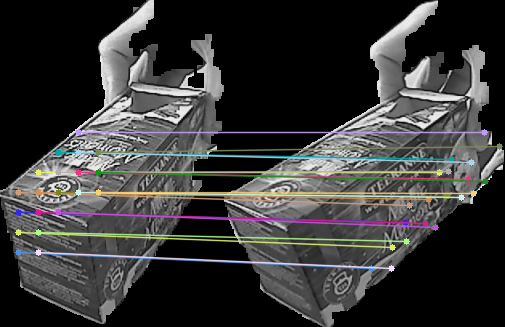
\includegraphics[width=300pt]{figures/vis_bad_0.png}
\caption{Első megközelítés (36 958 vektor) \label{fig:bad0}}
\end{figure}

A következő lépésem, hogy meghatározom azt a vektort, amivel eltolva az egyik képet, az egymásnak megfelelő képpontok elmozdulásai a lehető legkisebbek lesznek. Ehhez először szükségem van néhány egymásnak megfelelő pontpárra.

A SURF (Speeded Up Robust Features \cite{surf}) segítségével a képeken jellegzetes pontokat detektálhatunk és kiszámolhatunk ezek leíró vektorait, mely a pontokat és azok környezetét skála- és forgatás-invariáns módon azonosítja. Utóbbi tulajdonságra szükségünk is van, hiszen az objektumokról a képek más szögben és irányban készülnek. Ennek az implementációját OpenCV-ben a \texttt{cv::SURF} \cite{opencv-surf} osztályban találhatjuk, amely mind a pontok detekcióját, mind azok leírásának módját tartalmazza és megvalósítja.

Miután mindkét képen kinyertem a leíró vektorokat ezeket párosítanom kell. Ehhez a FLANN (Fast Approximate Nearest Neighbor Search Library \cite{flann_pami_2014}) könyvtárat használom, melyhez OpenCV-ben is elkészült az interfész \cite{opencv-flann}. Ennek segítségével gyorsan tudunk több dimenziós vektortérben egy vektorhoz (előzőkben kiszámolt leírók) megkeresni a hozzá legközelebbi vektort.

{\color{red} Valami kis implementációs dolog az osztályokról}

Annak ellenére, hogy a leírók nagyon hasonlóak, a párosításban szerepelhetnek rossz párok. Ismétlődő mintáknál előfordul, hogy két különböző pont képe nagyon közeli leíróvektort kap. Ezen a már használt epipoláris ($\mathbf{u}'^T \mathbf{F} \mathbf{u} = 0$) kényszert érvényesítve segítettem, azaz azokat a párokat kiszűrtem ahol az előző érték egy küszöbértéknél nagyobb. \Aref{fig:flann-matched}. ábrán látható a szűrés előtti és utáni párosítások.

\begin{figure}[tbh]
\centering
\begin{subfigure}[b]{.49\linewidth}
	\centering
	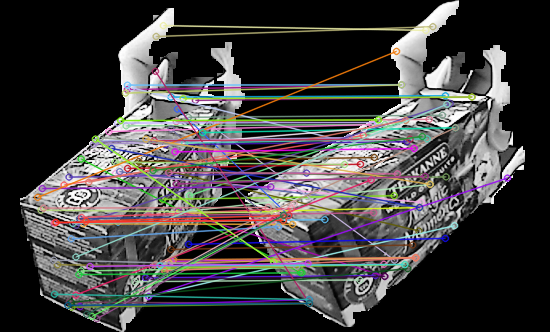
\includegraphics[width=205pt]{figures/matches_flann.png}
  \end{subfigure}
\begin{subfigure}[b]{.49\linewidth}
	\centering
	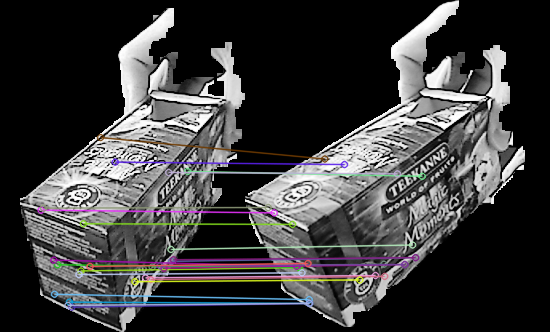
\includegraphics[width=205pt]{figures/matches_f.png}
  \end{subfigure}
\caption{Szűrés előtti (100 db) és utáni (25 db) párosítások a SURF és FLANN együttes használatával \label{fig:flann-matched}}
\end{figure}

Ezek után a párosítások jelentette vektorokból kell meghatároznom azt a vektort, amellyel az egyik képet eltolva az összetartozó pontok közötti távolság minimális. Azaz

\[\min_{\mathbf{v}(x, y)} \sum_{i=1}^{n} |\mathbf{v} - \mathbf{d_i}|\]

ahol $\mathbf{d_1}(x_1, y_1), \mathbf{d_2}(x_2, y_2), \ldots \mathbf{d_n}(x_n, y_n)$ a párosításban szereplő pontok közti távolságvektorok. Vagyis:

\[\min_{x, y} \sum_{i=1}^{n} \sqrt{(x-x_i)^2 + (y-y_i)^2}\]

{\color{red}Mivel a gyökvonás monoton, és a gyökvonás ezért a minimalizálásnál elhagyhatjuk. Így viszont ez megfogalmazható legkisebb négyzetek problémának, ami megoldható szinguláris érték szerinti felbontással.} \Aref{fig:shifted}. ábrán látható az eltolás előtt és után az objektum helyzete a két képen.

\begin{figure}[tbh]
\centering
\begin{subfigure}[b]{.49\linewidth}
	\centering
	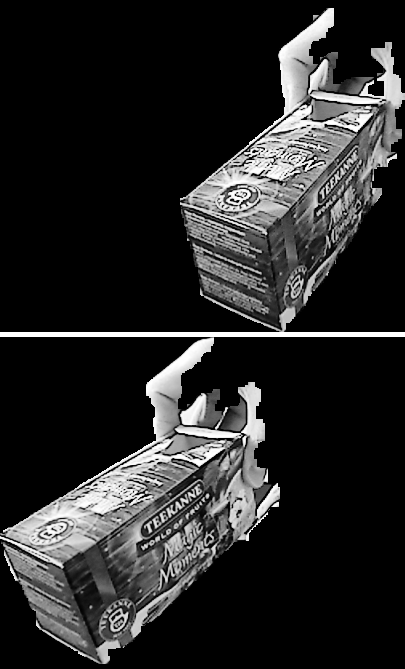
\includegraphics[height=205pt]{figures/before_shift.png}
  \end{subfigure}
\begin{subfigure}[b]{.49\linewidth}
	\centering
	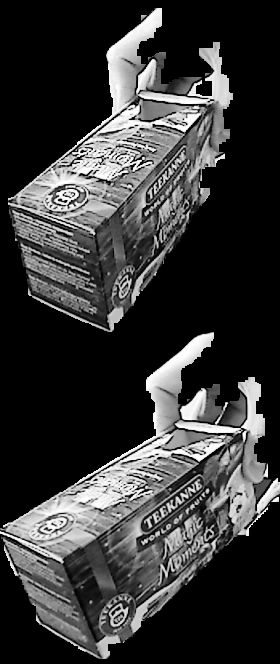
\includegraphics[height=205pt]{figures/after_shift.png}
  \end{subfigure}
\caption{Az objektum elhelyezkedése a kamerák képein (egymás alatt a két kamera képe) eredetileg és a kiszámolt vektorral való eltolás után. \label{fig:shifted}}
\end{figure}

Optikai folyamok számítása esetén két jelenséget nem szabad figyelmen kívül hagynunk: egyik a textúrázatlanság, a másik pedig a kitakart pontok problémája. Ezeken az optikai folyam rektifikációja segíthet. \cite{optical-flow-rectification}-ban You Yang és társai egy bináris függvényt javasolnak a textúrázatlanság eldöntésére:

\[
    \zeta(\Omega_\mathbf{X})= 
\begin{cases}
    0,              & \text{ha } \sigma(I_{\forall \mathbf{Y}\in\Omega_\mathbf{X}} - I_\mathbf{X}) < \varepsilon_\Omega\\
    1,              & \text{különben}
\end{cases}
\]

ahol $\Omega_\mathbf{X}$ jelöli $\mathbf{X}$ képpont egy környezetét, $I_\mathbf{X}$ az $\mathbf{X}$ pont intenzitását, $\sigma(.)$ a szórás-operátort egy halmazra nézve, valamint $\varepsilon_\Omega$ egy küszöbértéket, ami konstans. Úgy találták, hogy $\varepsilon_\Omega = 6$ választással jó eredményeket értek el, így én is ezt használtam. A mintaképek pontjaira kiszámolve ezt a függvényt, \aref{fig:textures}. ábrán látható maszkokat kaptam.

\begin{figure}[tbh]
\centering

\includegraphics[width=300pt]{figures/textures.png}
\caption{$\zeta$ függvény alkalmazva az objektum összes pontjára \label{fig:textures}}
\end{figure}

{\color{red}A kitakart pontok kiszűrésére én \cite{optical-flow-rectification}-től eltérő megközelítést alkalmaztam.} Legyen két képkocka $K_1$ és $K_2$, valamint $F_{1, 2} = \mathcal{F}(K_1, K_2)$ és $F_{2, 1} = \mathcal{F}(K_2, K_1)$, ahol $\mathcal{F}$ jelöli két képkocka közti optikai-folyam operátort, melynek eredménye egy vektormező ($F_{1, 2}, F_{2, 1} : \mathbb{R}^2 \rightarrow \mathbb{R}^2$). Gondoljuk meg, hogy ha $x\in K_1$ és $x + F_{1,2}(x) = x' \in K_2$, akkor $x' + F_{1,2}(x') \approx x \in K_1$, vagyis ha egy $x$ pont $K_1$-ről $K_2$-re az $x'$ pontba mozog, akkor visszafelé nézve $x'$ pontnak ideális esetben $x$ pontba kell, hogy mozogjon. Tehát oda-vissza számolva 1-1 optikai folyamot a kitakart pontokat kiszűrhetjük, hiszen a másik irányban nem fogjuk megtalálni a párosítást.

{\color{red} Valami implementációs dolog az egészről?}

Miután az előzőekben leírtakat felhasználtam és implementáltam, \aref{fig:vis_full}. ábrán kiemeltem néhány párosítást. Szabad szemmel is jól látható, hogy egész pontos párosításokat kaptam, összesen 16 841-et, tehát ennyi pontpárt tudunk majd a háromszögeléshez felhasználni. Vessük össze ezt a SURF leírókka történő párosításnál nyert 100, majd abból meghagyott 25 párral, számottevő a különbség.

\begin{figure}[tbh]
\centering
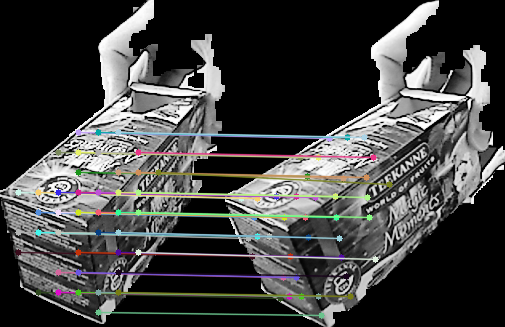
\includegraphics[width=300pt]{figures/vis_full.png}
\caption{Végső párosítás az optikai folyamok segítségével (16 841 vektor) \label{fig:vis_full}}
\end{figure}

%----------------------------------------------------------------------------
\section{Háromszögelés}
%----------------------------------------------------------------------------

Ahogy \aref{sec:triangulation}. alfejezetben bemutattam az elméleti hátteret, a következőkben ennek implementálását mutatom be.

\subsection{OpenCV-s függvényekkel}

OpenCV \texttt{cv::triangulatePoints} függvényben a \textit{Linear-LS} (lineáris legkisebb négyzetek) módszer van implementálva. Az interneten rákeresve több fórumban is találtam arra vonatkozó információkat, hogy sokan küzködnek ennek meghívásával. A dokumentáció \cite{camera-calib-3d} alapján sztereó-kalibráció során nyert projekciós mátrixokat várja a pontpárok mellett paraméterül. Az én esetemben, a kamerák nincsenek sztereó-kalibrálva, de a két projekciós mátrix megvan. Ennek ellenére a kimeneti 3D-s koordináták használhatatlanok voltak. Kis kutatás után az \texttt{cv::undistortPoints()} függvény meghívása jelentette a megoldást. Ez először normalizálta őket, vagyis:

\[\left(\begin{array}{c} u' \\ v' \\ 1 \end{array}\right) = {\underbrace{\left(\begin{array}{ccc}
f_x & 0 & o_x \\ 
0 & f_y & o_y \\
0 & 0 & 1
\end{array}\right)}_{\hbox{kamera-mátrix}}}^{-1} \left(\begin{array}{c} u \\ v \\ 1 \end{array}\right)\]

ahol $(u', v')$ az $(u, v)$ pont normalizáltja (kamera-mátrixtól független koordináták), majd a torzítási együtthatóakat felhasználva az $(u', v')$ pontoknak meghatározta a javított koordinátájukat. Ezután a \texttt{cv::triangulatePoints} függvénynek a projekciós mátrixok helyett csak az $\Big(\,\mathbf{R}\,|\,\mathbf{t}\,\Big)$ mátrixokat kellett átadnom. Fontos, hogy az előbbiekben kialakított pontpárosítás azon osztályához tartozó pontokat, melyek az eltolt képhez tartoznak, az eltoláshoz használt vektor ellentettjével vissza kell tolni, hogy valós koordinátákat kapjunk.

Miután megvannak a valóvilágbeli koordináták ezek pontosságát a képsíkokra történő visszavetítéssel vizsgáltam meg. A pontokat a \texttt{cv::projectPoints} függvénnyel vetítettem a bal oldali és jobb oldali kamera képére, majd a vetített és az eredeti pontok távolságainak átlagát -- átlagos visszavetítési hiba -- vizsgáltam. Ez az előzőekben mutatott bemenetre 8,68716 pixel lett, és \aref{fig:cv-triangulation}. ábrán látható az eredményeket bemutató két vizualizáció, melyeken a szín a pontok $z$ koordinátáját mutatja.

\begin{figure}[tbh]
\centering
\begin{subfigure}[b]{.49\linewidth}
	\centering
	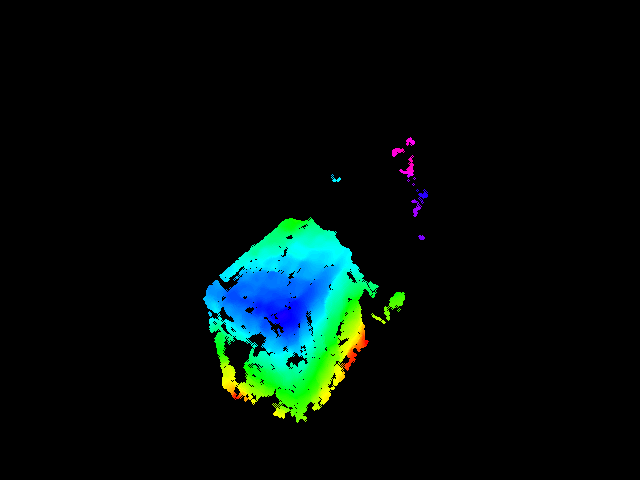
\includegraphics[width=205pt]{figures/visu_left.png}
	\caption{Bal oldali kamera nézőpontjából nézve \label{fig:cv-triangulation-a}}
  \end{subfigure}
\begin{subfigure}[b]{.49\linewidth}
	\centering
	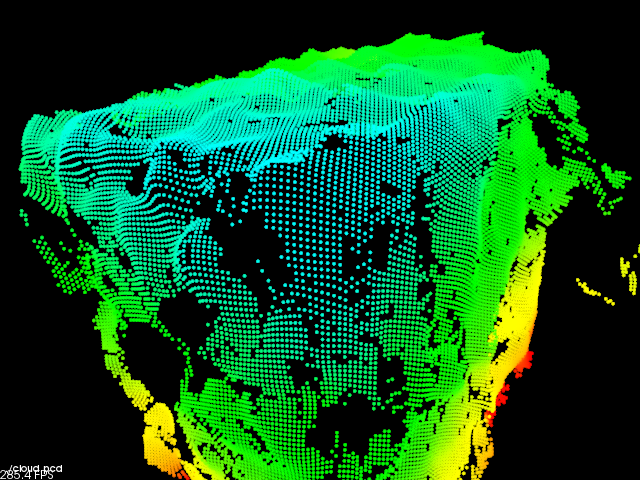
\includegraphics[width=205pt]{figures/visu_pcl.png}
	\caption{PCL vizualizációs szoftverrel ráközelítve}
  \end{subfigure}
\caption{Háromszögelés \textit{Linear-LS}-sel. Jól látható a közeli nézőpontból, hogy egy kissé hullámos lett a felület, de a pontatlanságra a hiba alapján számítottunk \label{fig:cv-triangulation}}
\end{figure}

Az OpenCV keretrendszerben megtalálhatjuk a \cite{hartley-triangulation}-ben leírt optimális, de polinomiális algoritmust is implementálva \texttt{cv::correctMatches()} néven, amely a fundamentális mátrix segítségével \aref{sec:triangulation}. szakaszban említett módon javítja a pontpárokat, azaz $\mathbf{u} \leftrightarrow \mathbf{u}'$ összerendelések helyett olyan $\mathbf{\hat{u}} \leftrightarrow \mathbf{\hat{u}}'$ párokat ad, melyekre $d(\mathbf{u}, \mathbf{\hat{u}})^2 + d(\mathbf{u}', \mathbf{\hat{u}}')^2$ minimális és teljesül, hogy $\mathbf{\hat{u}}'^T \mathbf{F} \mathbf{\hat{u}} = 0$. Ez az előbbi átlagos visszavetítési hibát 8,054 pixelre javította, de rohamos teljesítménycsökkenés mellett (0,06 másodperces futási idő helyett 0,64 másodperc lett, csak a háromszögelés), mely az eredményeket szabad szemmel megnézve nem meggyőző.


\subsection{Iteratív lineáris legkisebb négyzetek (\textit{Iterative-LS})}

\Aref{sec:triangulation}. szakaszban leírt iteratív módszert nem tudjuk alkalmazni a fenti \texttt{cv::triangulatePoints} függvénnyel, mert nem tudjuk az egyenleteket pontonként külön-külön súlyozni. Ennek megfelelően először a ,,szimpla'' \textit{Linear-LS} megközelítést kell implementálni, majd ezt már tudjuk majd iteratívan különböző súlyokkal meghívni.

Ehhez én Roy Shilkrot online elérhető alkalmazás-könyvtárából \cite{sfm-toy-library} merítettem a kiindulási alapot, és azt alakítottam az általam használt adatszerkezetekhez. Ehhez is előtte minden pontot normalizálni, valamint a torzítási együtthatóknak megfelelően javítani kellett. Ezzel a megközelítéssel 8,21 pixelnyi lett az átlagos visszavetítési hiba, de a sebesség harmadára csökkent (0,06 másodperc helyett 0,18 másodperc lett a futási idő), melyet szintén nem tekinthetünk kifizetődő kompromisszumnak.

A fentieket összegyűjtve a \texttt{Triangulator} osztályban (lásd \ref{fig:cd:triangulator}. ábra) implementáltam, melynek két metódusa a fent említett két módszert (OpenCV-s \texttt{triangulatePoints}, valamint az Iterative-LS) valósítja meg. Mindkettő az egymásnak megfelelő pontpárokat várja bemenetként, és harmadik paraméterében visszaadja az eredményt egy pontfelhőben, mely \texttt{CloudPoint}-ok vektoraként áll elő. Egy \texttt{CloudPoint} az aktuális koordinátákon kívül azt is tudja magáról, hogy mekkora a hozzátartozó visszavetítési hiba, így a megjelenítésnél eszerint tudunk is tudunk szűrni.

\begin{figure}[tbh]
\centering

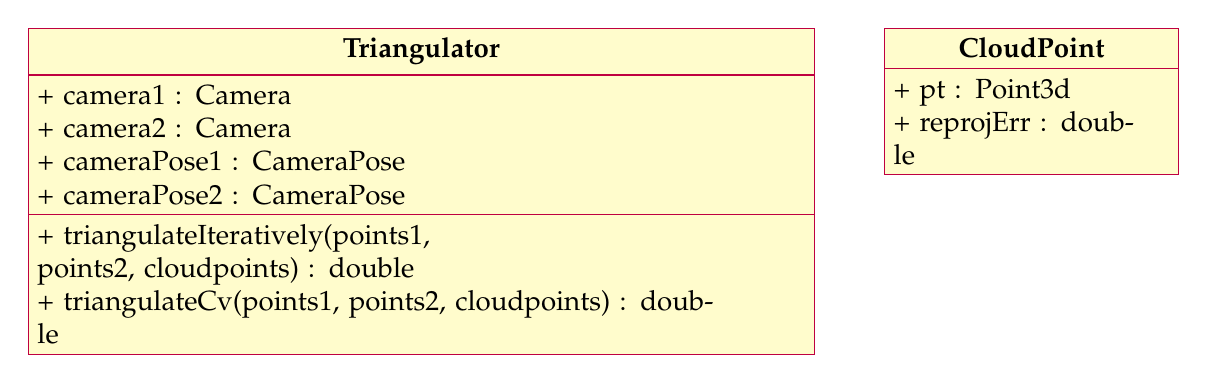
\begin{tikzpicture} 

\begin{class}[text width=9.75 cm]{Triangulator}{0, 0}
\attribute{+ camera1 : Camera}
\attribute{+ camera2 : Camera}

\attribute{+ cameraPose1 : CameraPose}
\attribute{+ cameraPose2 : CameraPose}

\operation{+ triangulateIteratively(points1, points2, cloudpoints) : double}
\operation{+ triangulateCv(points1, points2, cloudpoints) : double}
\end{class}

\begin{class}[text width=3.5 cm]{CloudPoint}{7.75, 0}

\attribute{+ pt : Point3d}
\attribute{+ reprojErr : double}

\end{class}

\end{tikzpicture}

\caption{\texttt{Triangulator} osztály és \texttt{CloudPoint} struktúra \label{fig:cd:triangulator}}
\end{figure}

%----------------------------------------------------------------------------
\section{Változtatható nézőpont}
%----------------------------------------------------------------------------

Ahogy az előbbiekben (lásd \ref{fig:cv-triangulation-a}. ábra) már említettem, a \texttt{cv::projectPoints} függvény segítségével lehet meghatározni, hogy adott kamerából fényképezve a valóvilágbeli pontoknak hol vannak a vetületei. Háromféle megjelenítési technikát implementáltam; \begin{inparaenum}[\itshape 1\upshape)]
\item $z$ koordinátát jelölő színkód,
\item eredeti képpontok színeinek felhasználása és
\item kontúrok rajzolása.
\end{inparaenum}

Az első implementálását a HSV (hue, saturation, value) színtér segítségével valósítottam meg. $S$ és $V$ értékét fixen a maximumra állítottam, $H$ értékét pedig egyenletesen elosztottam a különböző $z$ koordináták mentén.

A másodikhoz a pontfelhő mellé még két információra volt szükség: a pontok koordinátáira a bal képen, valamint a bal képre, hogy a pixelek színeit ki tudjam nyerni. Ezek után az adott 3D-s pont vetített képpontjának a színét a balképen lévő forrás pixel színére állítottam.

A harmadik megoldást 3 lépésben valósítottam meg. Először fehér pontokként levetítettem a pontokat a képsíkra. Ezt követően dilatáció-erózió kombinációval morfológiai zárást hajtottam végre a bináris képen, minek köszönhetően a kisebb lyukak és szakadások megszűntek. Végül az eredményen kontúrokat kerestem a \texttt{cv::findContours()} függvény segítségével, és ezeket kirajzoltam. Egy határérték (amit 100 pixel$^2$-nek választottam) alatti területtel rendelkező kontúrokat elvetettem, mert ezek kisebb olyan foltokat jelentenek, melyeket nem tudunk egyértelműen egy nagyobb objektumhoz rendelni.

Ezen három vizualizációjának eredménye a bal oldali kamera nézpontjából látható \aref{fig:different-vis}. ábrán.

\begin{figure}[tbh]
\centering
\begin{subfigure}[b]{.33\linewidth}
	\centering
	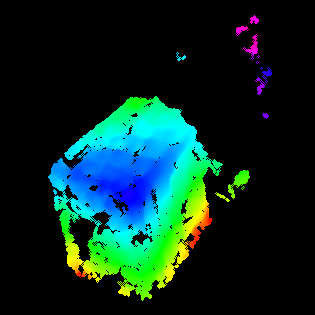
\includegraphics[width=135pt]{figures/visu_depth.png}
	\caption{Mélységinformáció}
  \end{subfigure}
\begin{subfigure}[b]{.32\linewidth}
	\centering
	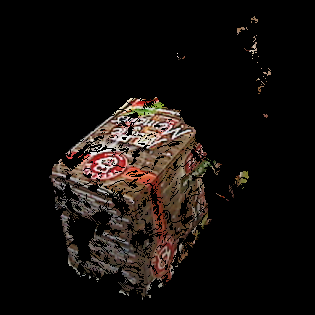
\includegraphics[width=135pt]{figures/visu_pixels.png}
	\caption{Eredeti pixelek}
  \end{subfigure}
\begin{subfigure}[b]{.32\linewidth}
	\centering
	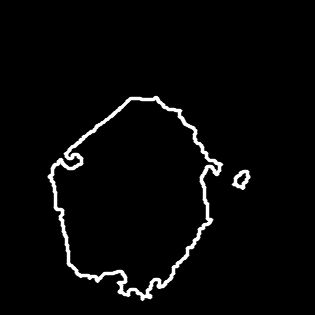
\includegraphics[width=135pt]{figures/visu_contours.png}
	\caption{Kontúrok}
  \end{subfigure}
\caption{Különböző vizualizációk, ráközelítve a hasznos területre \label{fig:different-vis}}
\end{figure}

Ahogy \aref{chapter3}. fejezetben említettem, a választott nézőpont, ahonnan érdemes lehet rekonstruálni az objektumot, a két kamera nézőpont között helyezkedhet el. Tehát a két kamera között szeretnénk interpolálni egy virtuális kamerát, és innen elvégezni a vetítést. Fontos, hogy nem elég csak a kamera helyzetét ($\mathbf{t_v}$), hanem a forgatási mátrixát ($\mathbf{R_v}$) is meg kell határozni. Jelölje $r \in [0; 1]$ a virtuális kamera pozícióját a pályáján, ahol $r = 0$, ha a bal oldali kamera, és $r = 1$, ha a jobb oldali kamera helyzetében van. Ekkor a virtuális kamera eltolási vektora $\mathbf{t_v} = (1-r)\mathbf{t_v} + r\mathbf{t_j}$, ahol $\mathbf{t_v}$ jelöli a bal oldali, $\mathbf{t_j}$ a jobb oldali kamera eltolási vektorát.
{\color{red} Kvaterniók...}


%----------------------------------------------------------------------------
\section{Eredmények, mérések, értékelés {\color{red} külön fejezet?}}
%----------------------------------------------------------------------------

{\color{red} Algoritmusok választása!!!}

%----------------------------------------------------------------------------
\section{Párhuzamosítás, többszálúsítás, újra-kalkulált eredmények}
%----------------------------------------------------------------------------



    %----------------------------------------------------------------------------
\chapter{Tesztelés, gyorsítási lehetőségek}
%----------------------------------------------------------------------------

A következő fejezetben egy kezdeti mérés után megvizsgálom azon lehetőségeket, amelyekkel gyorsítani lehet az elkészült implementáció működését. Először a párhuzamosítás lehetőségeit vizsgálom meg, majd kitérek a GPU-n történő számítási módszerekre, végül a bemeneti képek méreteinek változtatásának hatását vizsgálom meg a teljesítményre.

A teszteket egy olyan számítógépen végeztem, amiben egy Intel\textsuperscript{\textregistered} Core\texttrademark{} i5-4440 processzor és 8GB memória volt, és a kódot Linux operációs rendszerre fordítottam, és azon futtattam.

% -------------------------------------------------------
\section{Első mérések}
% -------------------------------------------------------

Elsőként egy olyan jeleneten próbáltam ki az elkészült alkalmazást, amely esetén a két kamera egymás mellett van (lásd \ref{fig:scene1_camerapose}. ábra), egy irányba néznek, és két teás dobozt mozgatok előttük. A jelenet 178 képkockából állt (\textasciitilde 5 másodperc), melyből mindegyik $640\times 480$-as felbontású, színes kép, 3 látható \aref{fig:scene1_frames}. ábrán. Az alkalmazást lefuttatva erre a jelenetre \aref{table:result_scene1_single}. táblázatban látható időket kaptam, lebontva a fontosabb lépésekre sorrendben, majd a teljes folyamatra is nézve. A legtöbb időt az optikai folyam meghatározása vitte el, utána az előtér maszkok, majd a textúrázottság meghatározása következett. Az átlagos visszavetítési hiba 0,806 pixelnyi lett az összes képkockára nézve. A teljes folyamat átlaga alapján 1 képkockapár rekonstrukciója majdnem 1 másodperc volt, azaz kb. 1,1 FPS sebességgel lehet rekonstruálni ezzel a megközelítéssel, ezen a hardveren, ilyen jellegű jelenet esetén. Megfigyelhető, hogy a bal oldali teás doboz rekonstrukciója a textúrázatlan területeken hiányos.

\begin{figure}[tbh]
\centering
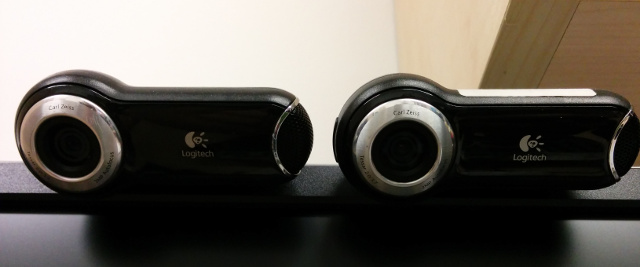
\includegraphics[width=300pt]{figures/scene1_camerapose.jpg}
\caption{Kamerák helyzete az első jelenetnél \label{fig:scene1_camerapose}}
\end{figure}

\begin{figure}[tbh]
\centering
\begin{subfigure}[b]{.32\linewidth}
	\centering
	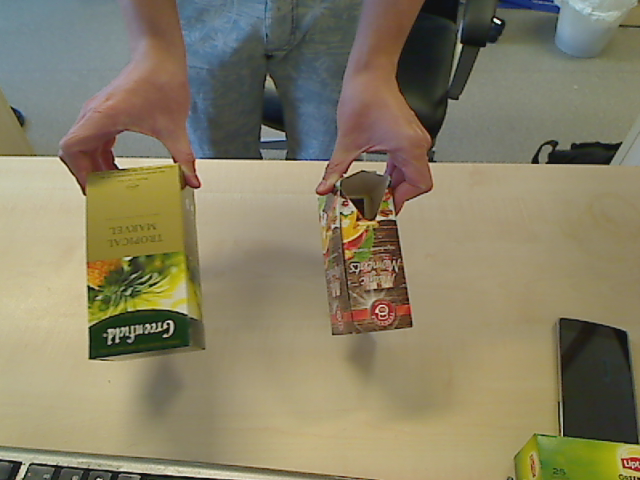
\includegraphics[width=135pt]{figures/left_93.png}
  \end{subfigure}
\begin{subfigure}[b]{.32\linewidth}
	\centering
	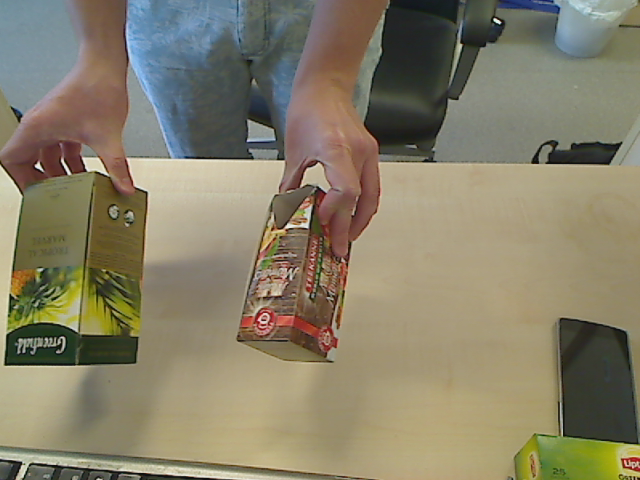
\includegraphics[width=135pt]{figures/left_153.png}
  \end{subfigure}
\begin{subfigure}[b]{.32\linewidth}
	\centering
	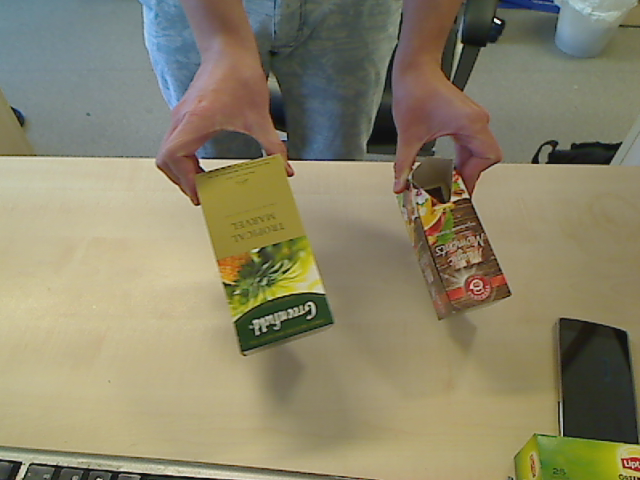
\includegraphics[width=135pt]{figures/left_223.png}
  \end{subfigure}\\\vspace{5pt}
\begin{subfigure}[b]{.32\linewidth}
	\centering
	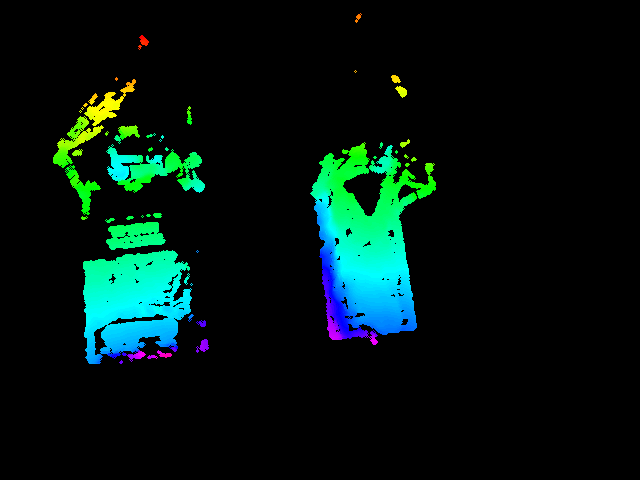
\includegraphics[width=135pt]{figures/vis_93.png}
  \end{subfigure}
\begin{subfigure}[b]{.32\linewidth}
	\centering
	\includegraphics[width=135pt]{figures/vis_153.png}
  \end{subfigure}
\begin{subfigure}[b]{.32\linewidth}
	\centering
	\includegraphics[width=135pt]{figures/vis_223.png}
  \end{subfigure}
\caption{A bal oldali kamera 3 képkockája (40., 100. és 170. képkocka) az első jelenetből, valamint a helyreállított képek a baloldali kamera nézőpontjából \label{fig:scene1_frames}}
\end{figure}

\begin{table}[tbh]
\centering

\begin{tabular}{|l|l|l|l|l|}
\hline
\multirow{2}{*}{Tevékenység képkockánként} & \multicolumn{4}{ |c| }{Eltöltött idő (s)} \\\cline{2-5}
 & min & max & átlag & szórás \\ \hline\hline

Előtér maszk (2 kamerára) & 0.039 & 0.229 & 0.178 & 0.0122 \\ \hline
Pontpárosítások ORB-bal & 0.0194 & 0.0629 & 0.0235 & 0.00474 \\ \hline
Objektumok párosítása & 0.0362 & 0.146 & 0.0583 & 0.0101 \\ \hline

Textúrázottság meghatározása & 0.0391 & 0.251 & 0.163 & 0.043 \\ \hline
Optikai folyam oda-vissza & 0.149 & 0.6 & 0.427 & 0.103 \\ \hline
Sűrű pontmegfeleltetések & 0.00222 & 0.0173 & 0.0119 & 0.00282 \\ \hline

Háromszögelés & 0.0008 & 0.0855 & 0.0587 & 0.0147 \\ \hline
Vizualizáció & 0.00226 & 0.0162 & 0.00845 & 0.00165 \\
\hline \hline
Teljes folyamat & 0.0695 & 1.16 & 0.908 & 0.17 \\ \hline
\end{tabular} 

\caption{Első jelenet esetén az egyes lépések futási idejükhöz kapcsolódó statisztikái (178 képkocka) \label{table:result_scene1_single}}
\end{table}


%----------------------------------------------------------------------------
\section{Párhuzamosítás, újra-kalkulált eredmények}
%----------------------------------------------------------------------------

Az előző szekcióban leírtak alapján látható, hogy szekvenciális végrehajtás esetén mekkora sebességet várhatunk az említett hardveren. A következőkben a párhuzamosításban rejlő lehetőségeket vizsgáltam meg.

Különböző platformokon, különböző megoldásokat találhatunk többszálú feladatvégrehajtásra. C++-ban az egyik legelterjedtebb az OpenMP API \cite{OpenMP, OpenMP-specs}. Felhasználásával platform-független, megosztott-memóriás párhuzamos programokat írhatunk. Nagy előnye, hogy ha a cél nem támogatja (legyen az a fordító, vagy a platform), akkor az API megfelelő alkalmazása esetén az alkalmazás ugyanúgy fordítható, azzal a különbséggel, hogy az elkészült bináris csak egy szálon hajtja végre az utasításokat. A következőkben röviden áttekintem az általam használt OpenMP funkciókat.

A többszálúság kezelése deklaratív alapon történik a \texttt{\#pragma omp} utasításokkal. Az első \texttt{\#pragma omp parallel} direktívánál egy fix számú szál-csapat jön létre (ami általában a CPU magjainak számától függ, de \texttt{num\_threads(N)} attribútummal ez kézzel is állítható), amely a program futása alatt konstans méretű. Ennek az az indoka, hogy a szálak létrehozása költséges folyamat, míg munkába állításuk nem.

A legegyszerűbb párhuzamosítási lehetőség, hogy az egymástól független lépéseket, amelyek ugyanazt csinálják (pl. két kamera két képéből külön-külön egy előtér meghatározása) \textit{for}-ciklusokba szervezzük, és ezek iterációit külön szálakon hajtjuk végre a \texttt{\#pragma omp for} utasítással. Hasonlóan a képek olyan feldolgozásakor (pl. textúrázottság vizsgálata), amikor egy iterációs lépés független a többitől, szintén használhatjuk ezt a módszert.

Az OpenCV (vagy az alatta lévő hardver-illesztő) a kamerák képeit buffereli, így ha az adott képkockákat nem tudjuk elég gyorsan lekérni, akkor beragadnak az egymás utániak, a későbbiek (amik nem férnek be a várakozási sorba) pedig elvesznek. Ha \textasciitilde{}30 FPS sebességgel rögzíti a képeket a kamera, akkor nagyjából 33ms időnk van egy képkocka feldolgozására. Mivel ezt nem sikerült elérni, így a következő ötletet alkalmaztam. Annak érdekében, hogy mindig azt a képkockát dolgozzam fel, amit éppen aktuálisan a kamera rögzít, a képek lekérését egy szálon folyamatosan végzem, és amikor éppen nem fut egy feldolgozás, akkor indítok egyet az aktuális képkockával. Ennek köszönhetően ugyan a feldolgozás nem folytonos, kimaradnak képkockák, viszont az adott rekontrukció a jelenlegi időponthoz nagyon közeli. A \texttt{\#pragma omp task} direktíva segítségével szerveztem a rekonstrukciót OpenMP feladattá, amely tulajdonképpen egy aszinkron végrehajtást jelent.

\definecolor{color1}{HTML}{4D4D4D}
\definecolor{color2}{HTML}{5DA5DA}
\definecolor{color3}{HTML}{FAA43A}
\definecolor{color4}{HTML}{60BD68}
\definecolor{color5}{HTML}{F17CB0}
\definecolor{color6}{HTML}{B2912F}
\definecolor{color7}{HTML}{B276B2}
\definecolor{color8}{HTML}{DECF3F}
\definecolor{color9}{HTML}{F15854}

\begin{figure}[b]
\centering
\begin{tikzpicture}
\begin{axis}[
    xbar stacked,
    legend style={
    legend columns=3,
        at={(xticklabel cs:0.5)},
        anchor=north,
        draw=none
    },
    ytick=data,
    axis y line*=none,
    axis x line*=bottom,
    tick label style={font=\footnotesize},
    legend style={font=\footnotesize},
    label style={font=\footnotesize},
    xtick={0.25, 0.5, 0.75, 1},
    width=.9\textwidth,
    bar width=6mm,
    xlabel={Idő másodpercben},
    yticklabels={1 szálon, több szálon},
    xmin=0,
    xmax=1,
    area legend,
    y=8mm,
    enlarge y limits={abs=0.625},
    legend cell align=left
]
\addplot[color1,fill=color1!40] coordinates {(0.178,1) (0.0944,0)};
\addplot[color2,fill=color2!40] coordinates {(0.0235,1) (0.0226,0)};
\addplot[color3,fill=color3!40] coordinates {(0.0583,1) (0.0296,0)};
\addplot[color4,fill=color4!40] coordinates {(0.163,1) (0.0749,0)};
\addplot[color5,fill=color5!40] coordinates {(0.427,1) (0.216,0)};
\addplot[color6,fill=color6!40] coordinates {(0.0119,1) (0.00618,0)};
\addplot[color7,fill=color7!40] coordinates {(0.0587,1) (0.042,0)};
\addplot[color8,fill=color8!40] coordinates {(0.00845,1) (0.0059,0)};

\legend{Előtér maszk, Pontpárosítások ORB-bal, Objektumok párosítása, Textúrázottság meghatározása, Optikai folyam oda-vissza, Sűrű pontmegfeleltetések, Háromszögelés, Vizualizáció}
\end{axis}  

\end{tikzpicture}
\caption{Első jelenet esetén az egyes lépések képkockánti átlagos időigénye másodpercben \label{fig:scene1_stats}}
\end{figure}

Ezekkel az apró javításokkal ellátva az alkalmazás kódját, \aref{table:result_scene1_multi}. táblázatban látható futási időket mértem az első jelenetre (itt még offline történt a feldolgozás, nem maradt ki egy képkocka sem). Az egyszálú végrehajtással összehasonlított átlagos idők \aref{fig:scene1_stats}. ábrán láthatóak. Megfigyelhető, hogy azon műveletek, amiket lehetett párhuzamosítani (pl. két képen ugyanazon művelet, két optikai folyam számolás), nagyjából kétszer gyorsabban fejeződtek be, a teljes folyamat pedig több, mint kétszeresére gyorsult. Ez annak köszönhető, hogy az objektumok rekonstrukcióit is párhuzamosítottam, ennek tudható be az is, hogy a teljes folyamat átlaga kisebb, mint a részfeladatok átlagainak szummája. Természetesen nem lehet a párhuzamosítással akármeddig gyorsítani, a rendelkezésre álló feldolgozóegységek korlátot szabnak az ésszerűen egymás mellett futtatható szálak számára, amely az én esetemben négy szál lett (ez pont ideális átlagosan két objektum/jelenet esetén).

\begin{table}[tbh]
\centering

\begin{tabular}{|l|l|l|l|l|}
\hline
\multirow{2}{*}{Tevékenység képkockánként} & \multicolumn{4}{ |c| }{Eltöltött idő (s)} \\\cline{2-5}
 & min & max & átlag & szórás \\ \hline\hline

Előtér maszk (2 kamerára) & 0.0875 & 0.103 & \textbf{0.0944} & 0.00261 \\\hline
Pontpárosítások ORB-bal & 0.0122 & 0.0368 & 0.0226 & 0.00347 \\\hline
Objektumok párosítása & 0.0206 & 0.0441 & 0.0296 & 0.00344 \\\hline

Textúrázottság meghatározása & 0.0208 & 0.11 & \textbf{0.0749} & 0.0153 \\\hline
Optikai folyam oda-vissza & 0.0731 & 0.312 & \textbf{0.216} & 0.0489 \\\hline
Sűrű pontmegfeleltetések & 0.000751 & 0.0122 & 0.00618 & 0.00147 \\\hline

Háromszögelés & 0.000567 & 0.058 & 0.042 & 0.0103 \\\hline
Vizualizáció & 0.00065 & 0.00838 & 0.0059 & 0.00138 \\
\hline \hline
Teljes folyamat & 0.109 & 0.574 & \textbf{0.391} & 0.105 \\ \hline

\end{tabular} 

\caption{Többszálú végrehajtás esetén az első jelenet feldolgozása során az egyes lépések futási idejükhöz kapcsolódó statisztikái (178 képkocka) \label{table:result_scene1_multi}}
\end{table}

%----------------------------------------------------------------------------
\section{Optikai folyam számolása GPU-n}
%----------------------------------------------------------------------------

OpenCV keretrendszerben néhány általam is használt eljárást a CUDA \cite{parallel-cuda} platformra is implementálták, melyeket egy külön \texttt{cv::cuda} névtéren belül találhatunk. Ezek segítségével, ha a videókártya támogatja, az algoritmusok implementációit a grafikus kártyán hatékonyabban futtathatjuk így növelve a teljesítményt.

\Aref{table:result_scene1_multi}. táblázatban láthatjuk, hogy az optikai folyam számolások, mind a sűrű pontmegfeleltetések számolásához, mind az előtér maszkhoz sok időt emésztenek fel. Miután feltelepítettem a CUDA Toolkit-et az NVIDIA honlapjáról \cite{cuda-nvidia}, újrafordítottam az OpenCV-t forrásból engedélyezve a CUDA modulokat. A GPU-s Färneback optikai folyam implementációját a \texttt{cv::cuda::FarnebackOpticalFlow} osztályban találhatjuk. Ezzel a módosítással további jelentős sebességnövekedést értem el, mely statisztikáit \aref{table:result_scene1_multi_gpu}. táblázat mutatja. Ezzel a megoldással az első jeleneten kb. 4 FPS-es feldolgozási sebességet értem el.

Az ORB-bal történő jellegzetes pontok detektálása és leírók számolása is történhet a GPU-n, viszont tesztelések alapján úgy tűnt, hogy ezek a műveletek nem szálbiztosak. A dokumentáció\cite{cuda-stream} is említi, hogy némelyik függvény konstans GPU buffert használ, így ugyanazon műveletek egymás utáni többszöri meghívása okozhat problémákat (az előző optikai folyam számolása úgy tűnik nem ilyen -- konkrét dokumentációt erről nem találtam). Sebességben ez kb. 0,01 másodpercet jelentett volna, annak kárára, hogy ezt a részt szálbiztossá teszem, így ezt az ötletet elvetettem.

\Aref{table:result_scene1_multi_gpu}. táblázatban jól látható, hogy jelenleg a legtöbb időt a textúrázottság meghatározása, valamint maga az optikai folyam kiszámolása viszi el. Utóbbin már nagyon nem lehet javítani, esetleg egy másik algoritmus választásával, előbbin pedig GPU-n történő számolással. Ezeket érdemes lenne a jövőben megvizsgálni.

\begin{table}[tbh]
\centering

\begin{tabular}{|l|l|l|l|l|}
\hline
\multirow{2}{*}{Tevékenység képkockánként} & \multicolumn{4}{ |c| }{Eltöltött idő (s)} \\\cline{2-5}
 & min & max & átlag & szórás \\ \hline\hline

Előtér maszk (2 kamerára) & 0.0304 & 0.0384 & \textbf{0.0337} & 0.00148 \\\hline
Pontpárosítások ORB-bal & 0.0176 & 0.0351 & 0.0262 & 0.00321 \\\hline
Objektumok párosítása & 0.0298 & 0.0477 & 0.0395 & 0.00328 \\\hline

Textúrázottság meghatározása & 0.0252 & 0.131 & 0.0886 & 0.0188 \\\hline
Optikai folyam oda-vissza & 0.0404 & 0.226 & \textbf{0.124} & 0.0405 \\\hline
Sűrű pontmegfeleltetések & 0.00101 & 0.0166 & 0.00773 & 0.00256 \\\hline

Háromszögelés & 0.000221 & 0.0561 & 0.0348 & 0.012 \\\hline
Vizualizáció & 0.00252 & 0.0106 & 0.00665 & 0.0016 \\
\hline \hline
Teljes folyamat & 0.137 & 0.338 & \textbf{0.259} & 0.0406 \\ \hline

\end{tabular} 

\caption{Többszálú végrehajtás és GPU-n történő optikai folyam számolás esetén az első jelenet feldolgozási statisztikája \label{table:result_scene1_multi_gpu}}
\end{table}


{\color{red}
%----------------------------------------------------------------------------
\section{Második jelenet}
%----------------------------------------------------------------------------

\ldots

}

%----------------------------------------------------------------------------
\section{Valós idejű helyreállíthatóság vizsgálata}
%----------------------------------------------------------------------------

A következőkben megvizsgálom, hogy milyen feltételek mellett érhető el a megvalósított megoldással valós idejű helyreállítás az átalam használt száímtógépen. A használt kamerákból \textasciitilde 30 FPS-es videófolyamok nyerhetőek, így akkor tekintettem valós idejűnek a feldolgozást, ha legalább 25 képkockát sikerült rekonstruálnom másodpercenként, közel-valós idejűnek pedig akkor, ha 15 képkockát. A következőkben megvizsgálom, hogy mekkora felbontás, valamint képen látható objektum-méret esetén érhető el a kívánt sebesség.

Először a képkockák méretét próbáltam csökkenteni a \texttt{cv::resize()} függvénnyel két lépésben, először $320\times 240$-es, majd $160\times 120$-as felbontásra. A sebességre jótékony hatással volt a képméretek csökkenése, viszont a rekonstrukció minőségére éppen ellenkezőleg. Azokon a képkockákon, ahol az objektumok helyben forogtak, de víszintes irányban nem sokat mozdultak értékelhetetlen lett a helyreállítás. Ez annak a következménye, hogy sok párosítás szempontjából fontos pont a kicsinyítés miatt eltűnt, illetve a képpontok eredeti mozgása a kisebb képeken elhanyagolható lett. Azonos képkockához tartozó rekonstrukciók eredményei és azok sebességei láthatóak \aref{fig:resize}. ábrán, amikor főleg csak vízszintes irányú mozgás történt. Ezek alapján sajnos nem sikerült elérni a valós idejű feldolgozást, csak a közel-valós idejűt, viszont jelentős minőségcsökkenéssel együtt.

\begin{figure}[tbh]
\centering
\begin{subfigure}[b]{.32\linewidth}
	\centering
	\includegraphics[width=137pt]{figures/vis_127_640.png}
	\caption{$640\times 480$; 3,86 FPS}
  \end{subfigure}
\begin{subfigure}[b]{.32\linewidth}
	\centering
	\includegraphics[width=137pt]{figures/vis_127_320.png}
	\caption{$320\times 240$; 12,2 FPS}
  \end{subfigure}
\begin{subfigure}[b]{.32\linewidth}
	\centering
	\includegraphics[width=137pt]{figures/vis_127_160.png}
	\caption{$160\times 120$; 18,2 FPS}
  \end{subfigure}
\caption{Egyre kisebb képkockák esetén a helyreállítás eredménye a bal oldali kamera nézőpontjából \label{fig:resize}}
\end{figure}

Ezt követően, a képkockák méretét nem kicsinyítéssel, hanem levágással csökkentettem. Az első jelenet esetében a képek érdemi része középen található, így először a középső $320\times 240$-es felbontású részt vettem figyelembe. Ekkor átlagosan 7,35 FPS-es sebességet értem el, mely főleg annak köszönhető, hogy a kisebb méret miatt általában csak 1 objektum látszódott, így csak egyet kellett rekonstruálni. \Aref{fig:cut_320_240}. ábrán látható ugyanazok képkockáknak a helyreállított vizualizációi, mint \aref{fig:scene1_frames}. ábrán.

\begin{figure}[tbh]
\centering
\begin{subfigure}[b]{.32\linewidth}
	\centering
	\includegraphics[width=137pt]{figures/vis_93_320.png}
  \end{subfigure}
\begin{subfigure}[b]{.32\linewidth}
	\centering
	\includegraphics[width=137pt]{figures/vis_152_320.png}
  \end{subfigure}
\begin{subfigure}[b]{.32\linewidth}
	\centering
	\includegraphics[width=137pt]{figures/vis_223_320.png}
  \end{subfigure}
\caption{Az első jelenet 40., 100. és 170. képkockájának a középső $320\times 240$-es képrészleteinek helyreállításai a bal oldai kamera nézőpontjából \label{fig:cut_320_240}}
\end{figure}
    %----------------------------------------------------------------------------
\chapter{Eredmények}
%----------------------------------------------------------------------------

Ebben a fejezetben az elért eredményeket összesítem és értékelem a megoldásom.

Az előző fejezet elején bemutattam az első jelenetet, amit teszteléshez használtam. Ez 178db $640\times 480$-as felbontású képből állt, melyeken két teásdobozt mozgattam, melyek mérete összesen kb. a képek területének 15\%-át tették ki. A bemutatott képeken jól látszódott, hogy a helyreállítás minősége a mélységet bemutató színábrázolással szemléltetve is nagyon jó lett, melyet az átlagos visszavetítési hibák (melyek átlaga 0,806 pixel lett) is jól alátámasztottak.

Ahogy a korábbi fejezetekben említésre került, a választott megoldáshoz szükséges, hogy az objektumok jól textúráltak legyenek, valamint azért, hogy a különböző objektumokat elkülöníthessem, egymáshoz képest is eltérő leírókkal (alak, szín, textúra jellege) kell rendelkezniük. Ezek az én esetemben nagyjából teljesültek, egyedül az egyik teásdoboz volt néhol túl homogén, de ez jól bemutatta a megoldás ezen korlátját.

A kezdeti 1 FPS-es sebességből párhuzamosítás és GPU-n történő gyorsítás után egészen 
3,86 FPS-re sikerült gyorsítani ugyanazon jeleneten a feldolgozás sebességét, amely jelentős növekedést jelent. Megvizsgáltam azt is, hogy kisebb képek esetén, mennyire közelíthető meg a kívánt valós idejű feldolgozás. A tesztek alapján úgy találtam, hogy az általam rendelkezésre álló hardveren a készített megoldás még az értékelhető $160\times 140$-es felbontás körüli képrészletekből jó minőségűnek vélt helyreállítást készített (ámbátor már jelentősebb, 5 pixeles átlagos visszavetítési hibával), és elérte a 12 FPS-es sebességet. De az elérni kívánt másodpercenkénti \textasciitilde 24 képkocka feldolgozását nem sikerült megközelíteni, ennél kisebb képeken pedig már nem volt gyakorlati haszna kísérletezni. Ezeken eredményeket összefoglalóan \aref{table:results}. táblázat mutatja be. {\color{red} Miért is lett lassabb a nem kicsinyített verzió??}

\begin{table}[tbh]
\centering

\begin{tabular}{|l|l|l|}
\hline
Módszer & felbontás & átlagos sebesség \\ \hline\hline

Egyszálon, CPU-n & $640\times 480$ & 1,1 FPS \\ \hline
Többszálon, CPU-n & $640\times 480$ & 2,56 FPS \\ \hline
Többszálon, GPU-n is & $640\times 480$ & \textbf{3,86 FPS} \\ \hline\hline

Eredeti kép kicsinyítve & $320\times 240$ & 12,2 FPS \\ \hline
Eredeti kép kicsinyítve & $160\times 120$ & 18,2 FPS \\ \hline\hline

Eredeti kép egy részlete & $320\times 240$ & 7,35 FPS \\ \hline
Eredeti kép egy részlete & $160\times 140$ & 12 FPS \\ \hline

\end{tabular} 

\caption{Egyes módszerek és különböző felbontás esetén az átlagosan elért sebesség \label{table:results}}
\end{table}


%----------------------------------------------------------------------------
\section{Továbbfejlesztési lehetőségek}
%----------------------------------------------------------------------------

\Aref{table:result_scene1_multi_gpu}. táblázatban jól látszódik, hogy a textúrázottság meghatározása sok időt emészt fel. Ezt GPU-ra megírva (CUDA vagy OpenCL kernel) jelentős sebességnövekedést várnék, amit érdemes lenne kivizsgálni. Ehhez viszont jobban meg kéne ismerni a heterogén párhuzamos programozás adta lehetőségeket.

Az OpenCV új verziójában átstruktúrált OpenCL-es implementációkat is jó lenne használatba venni, ugyan a dolgozatom során megpróbálkoztam vele, de sajnos sikertelenül. Elképzelhető, hogy ez a kész 3.0-s verzióban ez már gond nélkül fog működni.



    %----------------------------------------------------------------------------
\chapter{Eredmények}
%----------------------------------------------------------------------------

Ebben a fejezetben az elért eredményeket összesítem és értékelem a megoldásom.

Az előző fejezet elején bemutattam az első jelenetet, amit teszteléshez használtam. Ez 178db $640\times 480$-as felbontású képből állt, melyeken két teásdobozt mozgattam, ezek mérete összesen kb. a képek területének 15\%-át tették ki. A bemutatott képeken jól látszódott, hogy a helyreállítás minősége a mélységet bemutató színábrázolással szemléltetve is nagyon jó lett, melyet az átlagos visszavetítési hibák (melyek átlaga 0,806 pixel lett) is jól alátámasztottak.

Ahogy a korábbi fejezetekben említésre került, a választott megoldáshoz szükséges, hogy az objektumok jól textúrázottak legyenek, valamint azért, hogy a különböző objektumokat elkülöníthessem, egymáshoz képest is eltérő leírókkal (alak, szín, textúra jellege) kell rendelkezniük. Ezek az én esetemben nagyjából teljesültek, egyedül az egyik teásdoboz volt néhol túl homogén, de ez jól bemutatta a megoldás ezen korlátját.

A kezdeti 1 FPS-es sebességből párhuzamosítás és GPU-n történő gyorsítás után egészen 
3,86 FPS-re sikerült gyorsítani ugyanazon jeleneten a feldolgozás sebességét, amely jelentős növekedést jelentett. Megvizsgáltam azt is, hogy kisebb képek esetén, mennyire közelíthető meg a kívánt valós idejű feldolgozás. A tesztek alapján úgy találtam, hogy az általam rendelkezésre álló hardveren a készített megoldás még az értékelhető $160\times 140$-es felbontás körüli képrészletekből jó minőségűnek vélt helyreállítást készített (ámbátor már jelentősebb, 5 pixeles átlagos visszavetítési hibával), és elérte a 12 FPS-es sebességet. De az elérni kívánt másodpercenkénti \textasciitilde 24 képkocka feldolgozását nem sikerült megközelíteni, ennél kisebb képeken pedig már nem volt gyakorlati haszna kísérletezni. Ezen eredményeket összefoglalóan \aref{table:results}. táblázat mutatja be. Fontos megemlíteni, hogy a sebesség különbség az utolsó 2-2 esetben abból adódik, hogy amikor az eredeti kép egy részletét vizsgáltam, akkor a kép legnagyobb részét maga az objektum tette ki, míg a legkicsinyített verzióban csak egy kis részét.

\begin{table}[tbh]
\centering

\begin{tabular}{|l|l|l|}
\hline
\textbf{Módszer} & \textbf{Felbontás} & \textbf{Átlagos sebesség} \\ \hline\hline

Egyszálon, CPU-n & $640\times 480$ & 1,1 FPS \\ \hline
Többszálon, CPU-n & $640\times 480$ & 2,56 FPS \\ \hline
Többszálon, GPU-n is & $640\times 480$ & \textbf{3,86 FPS} \\ \hline\hline

Eredeti kép kicsinyítve & $320\times 240$ & 10,1 FPS \\ \hline
Eredeti kép kicsinyítve & $160\times 120$ & 14,3 FPS \\ \hline\hline

Eredeti kép egy részlete & $320\times 240$ & 7,7 FPS \\ \hline
Eredeti kép egy részlete & $160\times 140$ & \textbf{12 FPS} \\ \hline

\end{tabular}

\caption{Egyes módszerek és különböző felbontás esetén az átlagosan elért sebességek \label{table:results}}
\end{table}

A fentiek tükrében a feladat megoldása sikeresen, a kitűzött célt elérve valósult meg.

%----------------------------------------------------------------------------
\section{Továbbfejlesztési lehetőségek}
%----------------------------------------------------------------------------

\Aref{table:result_scene1_multi_gpu}. táblázatban (\pageref{table:result_scene1_multi_gpu}. oldal) jól látszódik, hogy a textúrázottság meghatározása sok időt emészt fel. Ezt GPU-ra megírva (CUDA vagy OpenCL kernel) jelentős sebességnövekedést várnék, amit érdemes lenne kivizsgálni. Ehhez viszont jobban meg kéne ismerni a heterogén párhuzamos programozás adta lehetőségeket.

Az előtér maszk meghatározása is jelentős időbe telik. Sajnos a gyorsabb MOG2 algoritmus rossz minőségű maszkokat eredményezett, bármilyen paraméterezéssel is próbálkoztam. Egy mélyrehatóbb vizsgálat lenne szükséges, hogy milyen egyéb megoldásokat lehetne itt alkalmazni, amely a teljes feldolgozás sebességét javítaná.

Érdemes lenne kipróbálni egyéb sűrű optikai folyamokat adó algoritmusokat is a meglévő mellett, hátha van olyan, ami hasonló eredményeket produkál ugyanazon hardveren kevesebb idő alatt. Erre Christopher Zach és társai \cite{zach2007duality} munkája egy jó alternatívának tűnik.

Az OpenCV új verziójában átstruktúrált OpenCL-es implementációkat is jó lenne használatba venni, ugyan a dolgozatom során megpróbálkoztam vele, de sajnos sikertelenül. Elképzelhető, hogy ez a kész 3.0-s verzióban már gond nélkül fog működni.



    {\color{blue}

%----------------------------------------------------------------------------
\chapter{Összefoglalás}
%----------------------------------------------------------------------------

A feladatkiírás pontjainak eleget tettem. Áttekintettem a szükséges irodalmat, elméleti hátteret, valamint megterveztem a megoldáshoz szükséges alkalmazást. Leírtam az implementálás részleteit, a hozott tervezői döntéseket, valamint kitértem a választott algoritmusok indoklására. Az elkészült alkalmazást két jeleneten teszteltem, a valós idejű feldolgozás korlátait megvizsgáltam, valamint részletesen dokumentáltam az eredményeket.

Az 1. fejezetben a feladat értelmezését követően a szükséges lineáris algebrai kitekintő után az alapvető háromdimenziós transzformációkat tárgyaltam. Végül a szakirodalomban és a dolgozat során is használt lyukkamera-modellel zártam, mely a kép- és videofeldolgozási algoritmusok alapjául szolgál.

A 2. fejezetben a több kamerából álló rendszereknél felmerülő, a feladatom során is megoldandó problémákat jártam körbe. Kitértem a kamerák szinkronizációjára, valamint a kamerák által látott képekből a háromdimenziós világ lehetséges rekonstrukciójára. Ehhez két lényegében eltérő megoldást vázoltam és mutattam be; a sztereó-kalibrációt valamint az optikai folyamokat. A fejezetet az objektum-detektálással zártam, mely felhasználásával a probléma megoldásának keresési tere csökkenthető. Az első két fejezettel a feladatkiírásom első pontjának eleget tettem.

A 3. fejezetben a célkitűzésem megfogalmazása után az előző fejezetekben megismert megközelítésekre és algoritmusokra támaszkodva megterveztem az elkészítendő rendszert.

A 4. fejezetben a megvalósítás lépéseit írtam le, az alkalmazás struktúráját osztály- és szekvencia diagramokkal szemléltettem, valamint az egyes fázisok eredményeit ábrákkal demonstráltam. Kitértem a megoldáshoz használt OpenCV-s függvényekre, valamint ezek paraméterezéseire.

Az 5. fejezetben az elkészült alkalmazást két jelenet segítségével teszteltem, melyek során két eltérő kamera telepítést alkalmaztam. Az eredményeket ábrákon keresztül bemutattam, valamint véleményt alkottam ennek minőségéről. Ezzel és az előző két fejezettel a feladatkiírásom második, valamint részben az utolsó pontjának tettem eleget.

A 6. fejezetben megvizsgáltam, majd alkalmaztam néhány lehetőséget, mellyel a teljesítmény javítható, ezeket mérésekkel is alátámasztottam. Végül megvizsgáltam, hogy milyen korlátok mellett, milyen sebesség érhető el. Az eredmények alapján azt találtam, hogy választható olyan kicsi, de még hasznos információval rendelkező képrészlet, mely esetén a közel valós idejű feldolgozás megvalósítható. Ezzel a feladatkiírásom utolsó két pontjának feleltem meg.

A 7. fejezetben tömören összesítem és értékelem az elért eredményeket, valamint kitérek a továbbfejlesztési lehetőségekre.

}

%\pagenumbering{roman}
%\setcounter{page}{\value{romanPage}}


% Acknowledgements
%~~~~~~~~~~~~~~~~~~~~~~~~~~~~~~~~~~~~~~~~~~~~~~~~~~~~~~~~~~~~~~~~~~~~~~~~~~~~~~~~~~~~~~


% List of Figures, Tables
%~~~~~~~~~~~~~~~~~~~~~~~~~~~~~~~~~~~~~~~~~~~~~~~~~~~~~~~~~~~~~~~~~~~~~~~~~~~~~~~~~~~~~~
	%\listoffigures\addcontentsline{toc}{chapter}{\abrakjegyzeke}
	%\listoftables\addcontentsline{toc}{chapter}{\tablazatokjegyzeke}


% Bibliography
%~~~~~~~~~~~~~~~~~~~~~~~~~~~~~~~~~~~~~~~~~~~~~~~~~~~~~~~~~~~~~~~~~~~~~~~~~~~~~~~~~~~~~~
    %\setlength{\bibitemsep}{5pt}

\dolgozatnyelve

	%----------------------------------------------------------------------------
\chapter*{\koszonetnyilvanitas}\addcontentsline{toc}{chapter}{\koszonetnyilvanitas}
%----------------------------------------------------------------------------

Végezetül szeretnék köszönetet mondani konzulensemnek, dr. Kovács Gábornak, aki folyamatosan támogatott, szakmai észrevételeivel és tanácsaival segítette munkámat. Sokat köszönhetek édesapámnak és barátaimnak, visszajelzéseikkel és javaslataikkal nagyban hozzájárultak a dolgozat elkészítéséhez.


    \printbibliography[title={\irodalomjegyzek}]
    \addcontentsline{toc}{chapter}{\irodalomjegyzek}
	

% Appendix
%~~~~~~~~~~~~~~~~~~~~~~~~~~~~~~~~~~~~~~~~~~~~~~~~~~~~~~~~~~~~~~~~~~~~~~~~~~~~~~~~~~~~~~
	%----------------------------------------------------------------------------
\appendix
%----------------------------------------------------------------------------
\chapter*{\fuggelek}\addcontentsline{toc}{chapter}{\fuggelek}
\setcounter{chapter}{6}  % a fofejezet-szamlalo az angol ABC 6. betuje (F) lesz
\setcounter{equation}{0} % a fofejezet-szamlalo az angol ABC 6. betuje (F) lesz
\numberwithin{equation}{section}
\numberwithin{figure}{section}
\numberwithin{lstlisting}{section}
%\numberwithin{tabular}{section}

%----------------------------------------------------------------------------
\section{Az alkalmazás elérhetősége}
%----------------------------------------------------------------------------

Az elkészült alkalmazás elérhető online egy Git tárolóban az alábbi címen: 

\url{https://github.com/messo/diploma}

Az alkalmazás C++ nyelven íródott, a platform független támogatást és a függőségek kezelését a CMake teszi lehetővé. Linuxon az alkalmazás a következő parancsok kiadásával fordítható:

\begin{lstlisting}[language=bash,basicstyle=\ttfamily\small]
   $ mkdir build && cd build
   $ cmake ..
   $ make -j4
\end{lstlisting}

A folyamat végén 3 bináris készül: \texttt{Calibration}, \texttt{PoseCalculation} és \texttt{Diploma}. Az elsővel generálhatóak a kamerák belső paramétereit tartalmazó fájlok, másodikkal a fix telepítésű kamerák elhelyezéseit számolhatjuk ki, majd a harmadik az előzőek által generált fájlok alapján a folyamatos helyreállítást végzi.


\label{page:last}
\end{document}
